%!TEX root = ../Thesis.tex

\chapter{Dynamic Formation Reconfiguration for On-Ramp Merging}
%\addcontentsline{toc}{part}{Introduction} % Adds "Introduction" as part-style in ToC
%\markboth{Introduction}{Introduction}    % Marks left and right headers as "Introduction"

\label{Chap04}
\begin{abstract}
In scenarios involving conflicting mergings, the decision-making component of the C-MCA is tasked with determining a secure passing sequence for the MVS within the merging zone. The passing sequence is subsequently translated into the MVS dynamics in the planning level through the application of the formation reconfiguration mechanism. Within this chapter, several dynamic formation reconfiguration approaches for on-ramp merging will be discussed. Each proposed formation reconfiguration will be outlined, and its performance will be assessed to identify any limitations. These identified limitations will then guide the refinement of the formation reconfiguration mechanism, iteratively improving it until the planning objectives of the C-MCA are satisfactorily met\footnote{The detailed contributions in this chapter have been the subject of the following publications \hyperlink{ITSC22}{ITSC'22}, \hyperlink{VAMS23}{VAMS'23},  \hyperlink{MMAR23}{MMAR'23} and  \hyperlink{ITSC23}{ITSC'23}.}.
\end{abstract}


\textbf{Contents}
\vspace{0.15cm}
\hline
\hspace{2cm}
\localtableofcontents
\hspace{2cm}
\hline












% In order to overcome the challenges related to the problem of on-ramp merging (cf. Section \ref{} \textcolor{red}{ajouter la reference de la section ou on parle de la complexité du on-ramp merging}), one consider the tackled scenario as a formation control problem. In other terms, the vehicles aiming to perform the merging maneuver as well as the highway can be seen as members of the same formation. Consequently, the formation need to be defined and configured, modeled, and perform the merging maneuver through the formation reconfiguration. 







% \subsection{Formation definition and configuration}\label{sec:formation_modeling_section}







% Based on the MVS paradigm \textcolor{red}{ajouter la reference de la section qui parle de l'état de l'art sur le MVS paradigm dans le chapitre 1} and the communication range of the RSU \textcolor{red}{ajouter la reference de la section qui parle des RSU ici}, a set of $N$ vehicles involved in creating the formation are identified. In other words, the RSU establishes connections with all the vehicles within its communication range. Consequently, the RSU assigns a unique communication identifier, in addition of the definition of the reference vehicle used as a reference frame by the formation coordinate system. This strategy is defined as follows: 

% \begin{itemize}
%     \item \textbf{Reference vehicle:} The RSU has the responsibility of designating the reference vehicle $V_R$ (cf. Figure \ref{fig:RSU-identification}). The pose of the later is used a mobile reference frame by the formation coordinates system. The RSU can select $V_R$ either from the vehicles part of the MVS or by considering a virtual vehicle. In this thesis work, the reference vehicle $V_R$ is selected from the MVS vehicles traveling in the lane containing the merging zone, and based on the shortest distance w.r.t. merging zone (cf. Figure \ref{fig:RSU-identification}). Its position is denoted by $x_{\text{R}}, y_{\text{R}}$, and its velocity by $\mathcal{V}_{\text{R}}$.
    
    
 

%     \item \textbf{Formation modeling approach:} The formation of MVS is structured based on the virtual structure approach (cf. Section \ref{} \textcolor{red}{ajouter la reference de la structure virtuelle}. In Figure \ref{fig:Coordinates_system} presents the formation coordinates  $F={f_i,i=1,\ldots,N}$, where $f_i$ are the $i-th$ vehicle coordinates w.r.t. the reference frame of the formation. 

    
% \end{itemize}
%        \begin{figure}[!h]
%         \centering 
%         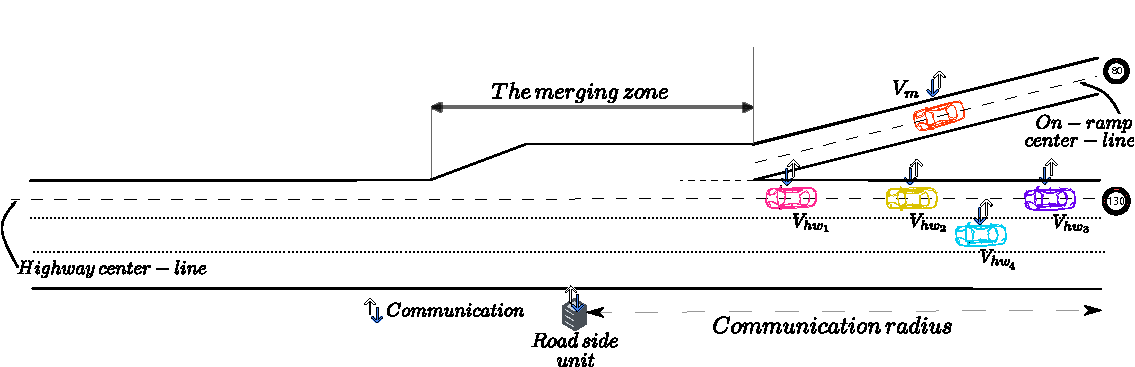
\includegraphics[width=14cm,height=6cm]{chapters/Chapitre_5/Figures/RSU_identification.pdf}
%         %\vspace{-2.3mm}
%         \caption{Formation identification and id attribution}
%         \label{fig:RSU-identification}
%         %\vspace{-5mm}
%         \end{figure}





% \subsubsection{Formation modeling based on a dynamic reference frame}


% In Figure \ref{fig:RSU-identification}, the RSU broadcast $V_{R}$ pose to the vehicles part of the formation in order to compute there coordinates w.r.t. $V_R$ reference frame. According to \cite{8430659}, two suitable frames for formation definition can be used: 


% \begin{itemize}
%     \item \textbf{Cartesian reference frame:} also called rigid formation, it is to maintain the formation's shape, the positions and orientations of the vehicles within the formation are computed relative to $V_{R}$, which also called the leader vehicle, with respect to the Cartesian frame (the local frame of the reference vehicle defined as $X_m$ and $Y_m$). This approach aims to reduce vehicle's dependence on a global reference frame. Applying a straightforward transformation allows the determination of the vehicles part of the formation coordinates within a local reference frame attached to the reference vehicle \cite{mariottini2007leader}\cite{benzerrouk2010navigation}.

%     \item \textbf{Frenet reference frame:} \label{sec:FrenetFrame} also known as flexible formation, this approach is utilized when it is more critical to track the reference vehicle's movements that to maintain a fixed formation shape during navigation. The Frenet reference frame is employed to adapt the formation to the reference vehicle's trajectory. This trajectory is used to define the formation's longitudinal (curvilinear) and lateral (perpendicular to the trajectory) coordinates \cite{8430659}\cite{avanzini2010urban}\cite{klanvcar2011control} (cf. Figure \ref{fig:Coordinates_system}).
% \end{itemize}








% In the Cartesian formation, the reference vehicle path is not taken into account such as in the Frenet formation, only its current Cartesian pose and dynamic have to be known by the vehicles part of the formation. since the reference vehicle trajectory is part of the Frenet formation modeling, the latter offers a safe formation navigation in static environment. In contrary, according to \cite{8430659}, the Cartesian formation allows a safe stable geometric formation shape. 

% During the on-ramp merging scenario the formation shape is reconfigured from one initial shape to another, while guaranteeing the safety of the reconfiguration. Based on the advantages of both of the formation modeling approaches, the Frenet modeling approach is the one that satisfy the scenario requirements. In fact, one of the particularities of the on-road environment is their dynamic, especially for highway environment. Additionally, the Frenet modeling approach offers more flexibility, an important requirement for navigation in dynamic environments. 

% \subsubsection{Formation modeling based on the Frenet reference frame}
% Each vehicle part of the formation is characterized by its coordinates $X_i=[x_i,y_i]^T$ within the global reference frame $[X_G,Y_G]$(cf. Figure \ref{fig:Coordinates_system}). In order to locate $X_i$ w.r.t. the reference vehicle $V_R$ (cf. Figure \ref{fig:Coordinates_system}), it is proposed to use a Frenet reference frame (cf. Section \ref{sec:FrenetFrame}) centered on $V_R$ (cf. Figure \ref{fig:Coordinates_system}). 

%        \begin{figure}[!h]
%         \centering 
%         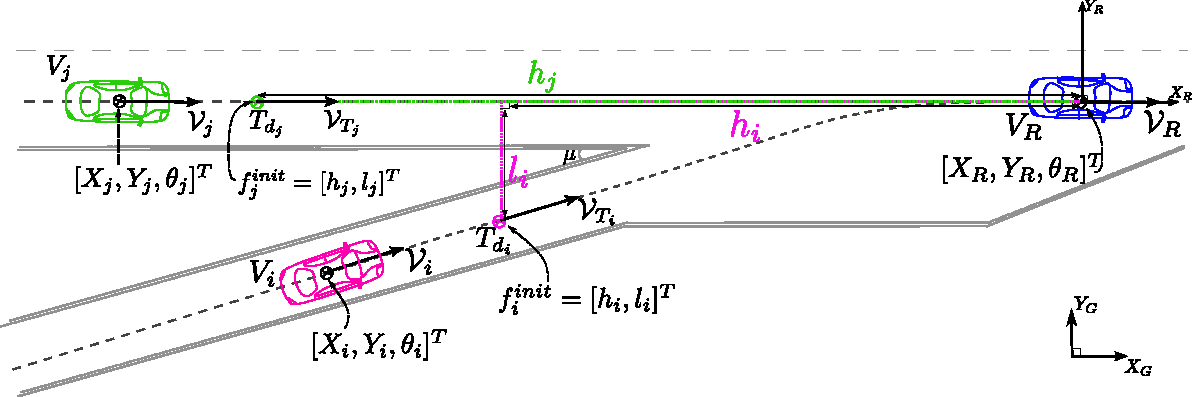
\includegraphics[width=14cm,height=18cm,keepaspectratio]{chapters/Chapitre_5/Figures/ModelingScenarioSimple.pdf}
%         %\vspace{-2.3mm}
%         \caption{Coordinates system based on the Frenet reference frame}
%         \label{fig:Coordinates_system}
%         %\vspace{-5mm}
%         \end{figure}



% According to $V_R$ pose $X_R$ and its reference trajectory (cf. Figure \ref{fig:Coordinates_system}) the coordinates system is described as follows: 

% \begin{itemize}
%     \item The $i-$vehicle coordinates part of the formation are defined as $f_i=[h_i,l_i]^T, i\in {N}$ (cf. Figure \ref{fig:Coordinates_system}). 

%     \item $h_i$ and $l_i$ are the longitudinal and lateral vehicle's coordinates w.r.t. the Frenet reference frame, respectively. The longitudinal coordinate $h_i$ represents the curvilinear distance between $V_R$ and $X_i$ according to the tangent to $V_R$ trajectory, while the lateral coordinate $l_i$ is computed based on the perpendicular line between $X_R(h_i)$ and its reference trajectory, and that passes through $X_i$, $l_i=PerpDist{X_R(h_i),X_i}$ (cf. Figure \ref{fig:Coordinates_system}). 
% \end{itemize}


% The kinematic model in eq. \ref{eq:kinematic model} \textcolor{red}{voir ou est le soucis avec cette equation} is written in the global reference frame ${X_G, Y_G}$, thus a transformation from the mobile reference frame to the global reference frame is obtained with the following equations: 

% \begin{equation} \label{eq:frenetToCartisian}
% \begin{matrix}
% \begin{bmatrix}
% x_{T_i} \\
% y_{T_i} \\
% \end{bmatrix}
% & = & \begin{bmatrix}
% x_{R}(h_i)\\
% y_{R}(h_i) \\
% \end{bmatrix}
% & + & \begin{bmatrix}
% -l_i\sin(\theta_R(h_i)) \\
% l_i\cos(\theta_R(h_i)) \\
% \end{bmatrix}
% \end{matrix}
% \end{equation}


% with $[x_{T_i},y_{T_i}]^T$ is the i-th vehicle virtual target w.r.t. $V_R$'s mobile reference frame. $[x_R,y_R]^T$ and $\theta_R$ are the reference vehicle $V_R$ pose and orientation.



  






\section{Introduction}




The key concept behind the proposed dynamic formation reconfiguration approach is to take advantage of the MVS coordination ability to achieve safely and smoothly the merging scenario. In other terms, dynamic formation reconfiguration is used to control the vehicles motion during the merging phase. 

Once the ${N}\in \mathbb {N}$ vehicles part of the formation are identified, the Frenet frame (cf. Section \ref{sec:FrenetFrame}) is used to model the initial shape $F^{init}$. The formation desired shape $F^{end}$ (cf. Figure \ref{fig:Coordinates_system_full_scenario}) is obtained through the translation of the passing sequence $sq$ selected by the decision-making level. Lastly, in order to perform the merging maneuver, the formation reconfiguration process is launched. 

     \begin{figure}[!h]
        \centering 
        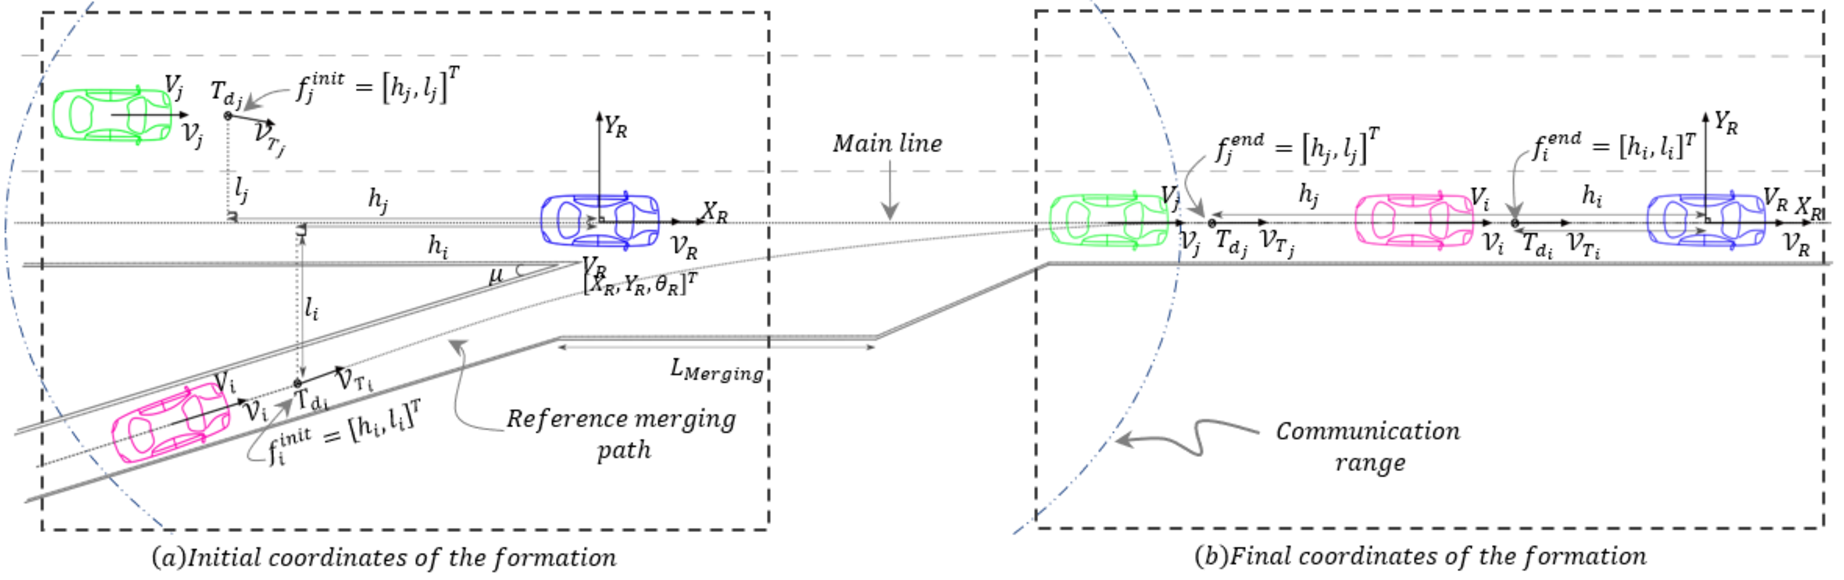
\includegraphics[width=13cm,height=6cm]{chapters/Chapitre_5/Figures/FullMergingScenario.pdf}
        %\vspace{-2.3mm}
        \caption{The virtual structure approach used to model the formation and its reconfiguration to perform the merging maneuver. (a) The initial shape of the formation and its coordinates. (b) The final shape of the formation after the merging maneuver and its desired coordinates. }
        \label{fig:Coordinates_system_full_scenario}
        %\vspace{-5mm}
        \end{figure}

Formation reconfiguration is the process that reshapes the formation from its initial shape $F^{init}$ toward the final one $F^{end}$ by generating intermediary formation coordinates $F(t)$ (cf. Figure \ref{fig:Coordinates_system_full_scenario}). The intermediary coordinates are transformed from the Frenet frame to the global Cartesian frame to generate the vehicles virtual targets $T_d$. The respect of the merging safety is ensured with the help of the inter-vehicle target distances. In other terms, each vehicle part of the MVS has its own virtual target $T_d$ generated by the formation reconfiguration process. The distance between two targets is the inter-vehicle target distances. Consequently, the MVS safety during the merging is ensured by the generation of safe virtual targets. The system of equations that describes the formation reconfiguration are given below: 
    


\begin{equation}\label{eq:initialandfinalcoordinates}
\begin{cases}
F^{init}=[f_{1}^{{init}^T}, ...,f_{N}^{{init}^T}]^T, \\
F^{end}=[f_{1}^{{end}^T}, ...,f_{N}^{{end}^T]^T},\\
F(t)=[f_{1}(t)^T, ...,f_{N}(t)^T]^T,
\end{cases}
\end{equation}

$f_i ^{init},f_i ^{end}, i\in {N}$ are the coordinates of $V_i$ in the initial and final formation, while $f_{i}(t), i\in{N}$ are its instantaneous coordinates. 

$e_{f_{i}}=[e_{h_{i}},e_{l_{i}}]^T $ is the convergence error between the desired coordinates of $V_i$ in the formation and the actual ones, it can be defined as: 

\begin{equation}\label{eq: errorbetweenfinitandfendforvi}
\begin{cases}
    e_{f_{i}}=f_{i}^{end} - f_{i}(t),\\
    f_{i}(t)=[h_{i}(t), l_{i}(t)]^T,\\
    f_{i}^{end}=[h_{i}^{end},l_{i}^{end}]^T,
\end{cases}
\end{equation}

The global error for a formation composed of ${N}$ vehicles can be written as: 
\vspace{-2.3mm}
\begin{equation}
    e_{F}=F^{end} - F(t)
\end{equation}

The derivative expression of the error can be written as: 
\begin{equation} \label{eq:fct error}
    \dot{e}_F=g(e_{f_{1}}, ..., e_{f_{N}})
\end{equation}


Equation \ref{eq:fct error} describes the formation reconfiguration problem as a control problem, where the goal is to control the convergence error from its initial value (error with the initial formation shape) toward the final one (error with the desired shape, so zero), while ensuring the respect of the vehicles' safety. 

 Part of this research work, several formation reconfiguration approaches were proposed. The following sections aim to describe these approaches. In Section \ref{sec:CORM}, the Constrained Optimal Reconfiguration Matrix (CORM) is described along with its advantages and limitations. Based on the CORM's limitations, the Extended Constrained Optimal Reconfiguration Matrix (E-CORM) was proposed (cf. Section \ref{sec:E-CORM}). Lastly, in order to overcome both the CORM's and the E-CORM's limitations, the Formation Reconfiguration Approach based on an Online Control Strategy (FRA-OCS) is proposed and presented in Section \ref{sec:No-opt}. The performance of each of the proposed formation reconfiguration approaches is discussed with the help of several simulation results. 





    
 \section{Constrained Optimal Reconfiguration Matrix (CORM)} \label{sec:CORM}  



The proposed Constrained Optimal Reconfiguration Matrix (CORM) involves an analysis of the derivative of $e_F$ (cf. eq. \ref{eq:fct error}). This analysis aims to ensure convergence to the new formation shape and generates smooth trajectories using the virtual targets during the reconfiguration process. Additionally, it helps to manage the minimum inter-target distance to prevent collisions between vehicles. 

The CORM is originally inspired by the inter-target distance matrix, thus, a concise overview of the latter is presented in the following section. Subsequently, the section focuses on the Constrained inter-target distance matrix proposed to explicitly take into account the road constraints. Lastly, this section delves into the safe and feasible local trajectory planning strategy proposed to ensure the feasibility of the formation reconfiguration during the merging. 



\subsection{The inter-target distance matrix} \label{sec:Inter-target-distance-matrix}

The proposed function $\dot{e}_F$ for the entire formation is adapted from \cite{ventura2015safe}\cite{8430659}, and it is designed as a linear system: 

\begin{equation}\label{eq:linearSystem}
    \dot{e}_{F}= Ae_F
\end{equation}

where $e_F=[e_{f_{1}}^T, ..., e_{f_{N}}^T]^T$ and $A^{2N \times 2N}$ are the state vector and the inter-target distance matrix corresponding to a formation of $N$ vehicles, respectively. 

\begin{equation}\label{eq: reconfiguration matrix}
A = 
 \begin{bmatrix}
  a_{1}I^{2 \times 2} & a_{12}I^{2 \times 2} & \cdots & a_{1N}I^{2 \times 2} \\
  -a_{12}I^{2 \times 2} & a_{2}I^{2 \times 2} & \cdots & a_{2N}I^{2 \times 2} \\
  \vdots  & \vdots  & \ddots & \vdots  \\
  -a_{1N}I^{2 \times 2} & -a_{2N}I^{2 \times 2} & \cdots & a_{N}I^{2 \times 2} 
 \end{bmatrix}
\end{equation}

The gains $a_{i}$ on the diagonal with $ i\in N $ control the convergence rate of the error, while  $a_{ij}$ with $i\neq j | \forall i,j\in \{N\times N\}$ are related to the inter-target distance between $T_{d_{i}}$ and $T_{d_{j}}$, to ensure the convergence of the formation toward its desired shape. 


The stability of the formation error system can be straightforward proved using Lyapunov analysis with the Lyapunov candidate function: 

\begin{equation}\label{eq:lyapunovFunction_CORM}
    V=\frac{1}{2}e_F^Te_F
\end{equation}

$V$ is a positive-definite function. To guarantee the stability of the system, $\dot{V}$ must be negative-definite. By taking the derivative of eq. \ref{eq:lyapunovFunction_CORM} and using eq. \ref{eq:linearSystem}, $\dot{V}$ can be written as: 

\begin{equation}\label{eq:derivativeLyapuniov_CORM}
    \dot{V}=e_F^T\dot{e}_F=e_F^TAe_F
\end{equation}

Since $A$ is negative-definite, then $\dot{V}<0$ and the formation error system has an asymptotic convergence. 

\subsubsection*{Safety insurance}


It is important to highlight that to avoid the collisions between the $N$ vehicles part of the formation, the condition relating the minimum inter-distances $\underline{D}_{T}$ and the gains of the matrix $A$ must be satisfied. Indeed, the distance between the defined target set-points must be greater than a certain constant minimum distance, called $\underline{D}_{T}$. The latter is chosen to take into account the dimensions of the vehicle in addition to a certain offset (cf. Figure \ref{fig:safetydistance}). 


       \begin{figure}[!h]
        \centering 
        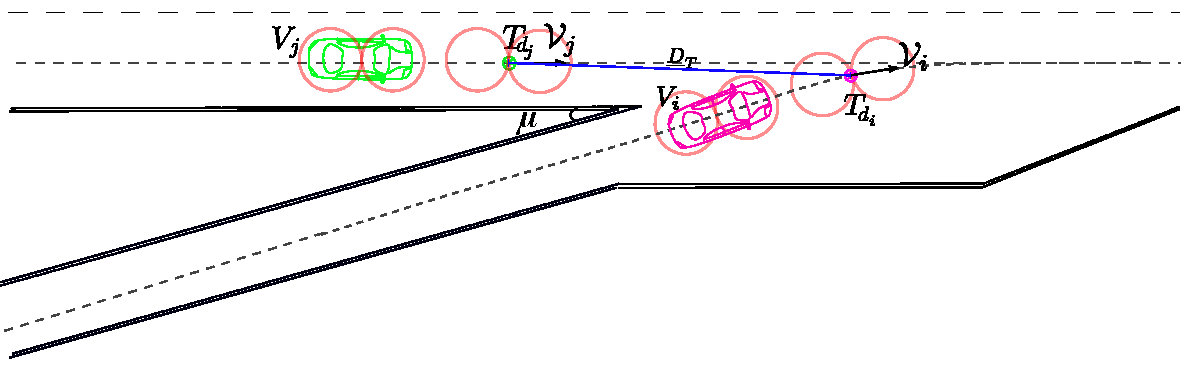
\includegraphics[width=10cm,height=5cm]{chapters/Chapitre_5/Figures/safety_distance.pdf}
        %\vspace{-2.3mm}
        \caption{Illustration of the merging scenario where the minimum inter-distance $\underline{D}_{T}$ is depicted}
        \label{fig:safetydistance}
        %\vspace{-5mm}
        \end{figure}




For example, the case of two targets $T_{d_2}$ and $T_{d_3}$ is analyzed. The inter-target distance can be computed as: 

\begin{equation}\label{eq:derivative_inter_target}
    d_T^2 = e_{f_{23}}^Te_{f_{23}}
\end{equation}


Taking the derivative of the last equation to obtain the minimum value: 
\begin{equation} \label{eq:nul_distane_derivative}
    2e_{f_{23}}^T\dot{e}_{f_{23}}=0
\end{equation}

After several developments (the details can be found in Appendix \hyperlink{AppendixB}{B}), it is obtained finally in order to respect the minimum inter-target $\underline{D}_T$ \cite{8430659}: 

\begin{equation}\label{eq:FinalDistaneStudy_2}
    e_{f_{23}}^T \Big[\frac{a_2-a_3+a_{23}}{a_3-a_{23}}{e}_{f_2} + {e}_{f_{23}}^{end} \Big] \geq \underline{D}_{T} ^2 
\end{equation}

Thus, the values of $a_2$, $a_3$, and $a_{23}$ must be chosen to satisfy eq. \ref{eq:FinalDistaneStudy_2}.




The inter-target distance matrix proposed in \cite{8430659} is designed for an open-world environment, where a reactive collision avoidance approach was used only against the other moving robots present in the environment. Nevertheless, in the proposed CORM, it is targeted to deal with structured on-road environment, with road borders (cf. Figure \ref{fig:Coordinates_system_full_scenario}). It is thus important that the proposed formation reconfiguration takes into account these constraints. In order to take explicitly into account these road constraints while reconfigurating the MVS formation during the merging maneuver the constrained inter-target distance matrix is proposed. The details of the proposed approach are given in the following section.  


\subsection{Constrained inter-target distance matrix}
In on-road environment, the vehicles travel in a constrained environment, imposed by the road borders and the road geometry. As stated in Section \ref{sec:Inter-target-distance-matrix}, the inter-target distance matrix proposed in \cite{8430659} do not takes environments with such constraints into account. In order to mitigate these constraints, it is proposed a two-steps reconfiguration matrix computation. 

First, through an optimization algorithm (cf. Section \ref{sec:CORM_optimization_alg}), it is proposed to compute a constrained inter-target distance matrix. Consequently, the virtual targets $T_d$ of the $N$ vehicles part of the formation can be generated. This ensures the reconfiguration of the formation from the initial shape to the desired one, through the merging maneuver (cf. Figure \ref{fig:Coordinates_system_full_scenario}), while guaranteeing the respect of the safety distance between the vehicles. The geometry of the road (i.e., the road borders and the road center-line) is taken into account at this level with the help of an optimization process based on the objective function given by eq. \ref{eq:costfunction}. In Section \ref{sec:CORM_optimization_alg}, the details of this first step are presented. 


The constrained optimization in the first step allows to generate $\mathcal{M}$ (cf. Figure \ref{fig:CORM-approximation}); an approximation of the global reference trajectory w.r.t. the objective function given in eq. \ref{eq:costfunction}. However, the targets $T_d$ are not guaranteed to be onto the reference path (cf. Figure \ref{fig:CORM-approximation}), thus, in the second step of the proposed formation reconfiguration approach, it is proposed to project these generated virtual targets w.r.t. the reference path. The projection uses a Frenet reference frame w.r.t. the reference path to obtain the projected targets $T_p$. The dynamic of the projected targets $T_p$ is similar to the one of $T_d$, which means that if the vehicles follow precisely $T_p$, the vehicles stay on their reference path. However, their in-between distance profile will not be the same as if they follow $T_d$. Thus, it is proposed to impose a new dynamic to $T_p$ to obtain $\overline{T}_p$. The latter makes sure that the vehicles are at the same safety distance as the one obtained with the constrained inter-target matrix when they enter the conflicting zone (cf. Figure \ref{fig:CORM-approximation}). Section \ref{sec:Projected_target} gives the details of the computation of the projected target and its dynamic. 

\subsubsection{Constrained optimal reconfiguration matrix} \label{sec:CORM_optimization_alg}
The objective of the optimization algorithm presented in what follows is to compute the optimal constrained inter-distance matrix w.r.t. the objective function in eq. \ref{eq:costfunction}. 




\begin{align} \label{eq:costfunction}
J_{\substack{ a_{k} \\\forall k  \in {N}}} = \sum_{k=0}^{T} \Bigg[ &w_{i}\Big[\frac{PerpDist\{T_{d_{i}}(k),{T}_{p_{i}}(k)\}}{PerpDist\{{T}_{p_{i}}(k),Border\}}\Big]^2 + \nonumber \\  
&w_{j}\Big[\frac{PerpDist\{T_{d_{j}}(k), {T}_{p_{j}}(k))}{PerpDist\{{T}_{p_{j}}(k),Border\}}\Big]^2\Bigg]
\end{align}

Equation \ref{eq:costfunction} is composed of two terms: The first term takes into account the $i-th$ vehicle, it aims to minimize distance between $V_i$'s reference path and $T_{d_i}$ (cf. Figure \ref{fig:CORM-approximation}), while the second term related to the $j-th$ vehicle, considers the minimization of distance between $T_{d_j}$ and its reference path (cf. Figure \ref{fig:CORM-approximation}). $w_i$ and  $w_j$ with $w \in  \mathbb{R}^{+}$, correspond to the optimization weights balance between the two sub-criteria, the weight related to the merging vehicle is higher in order to give the latter a sufficient flexibility w.r.t. to the vehicles already on the main line. For $i\neq j, \forall i,j \in {N}$, $T_{d_{i,j}}$ and $T_{p_{i,j}}$  are the targets obtained with constrained inter-target distance matrix and their projected points respectively (cf. Figure \ref{fig:CORM-approximation}). $PerpDist\{T_{d_{i,j}}(k),{T}_{p_{i,j}}(k)\}$ are the perpendicular distances between $T_d$ and its projected target $T_p$ w.r.t. to the reference path, while $PerpDist\{{T}_{p_{i,j}}(k),Border\}$ are the perpendicular distances between the projected target and the road border, used to normalize the objective function (cf. Figure \ref{fig:CORM-approximation}). 



       \begin{figure}[!h]
        \centering 
        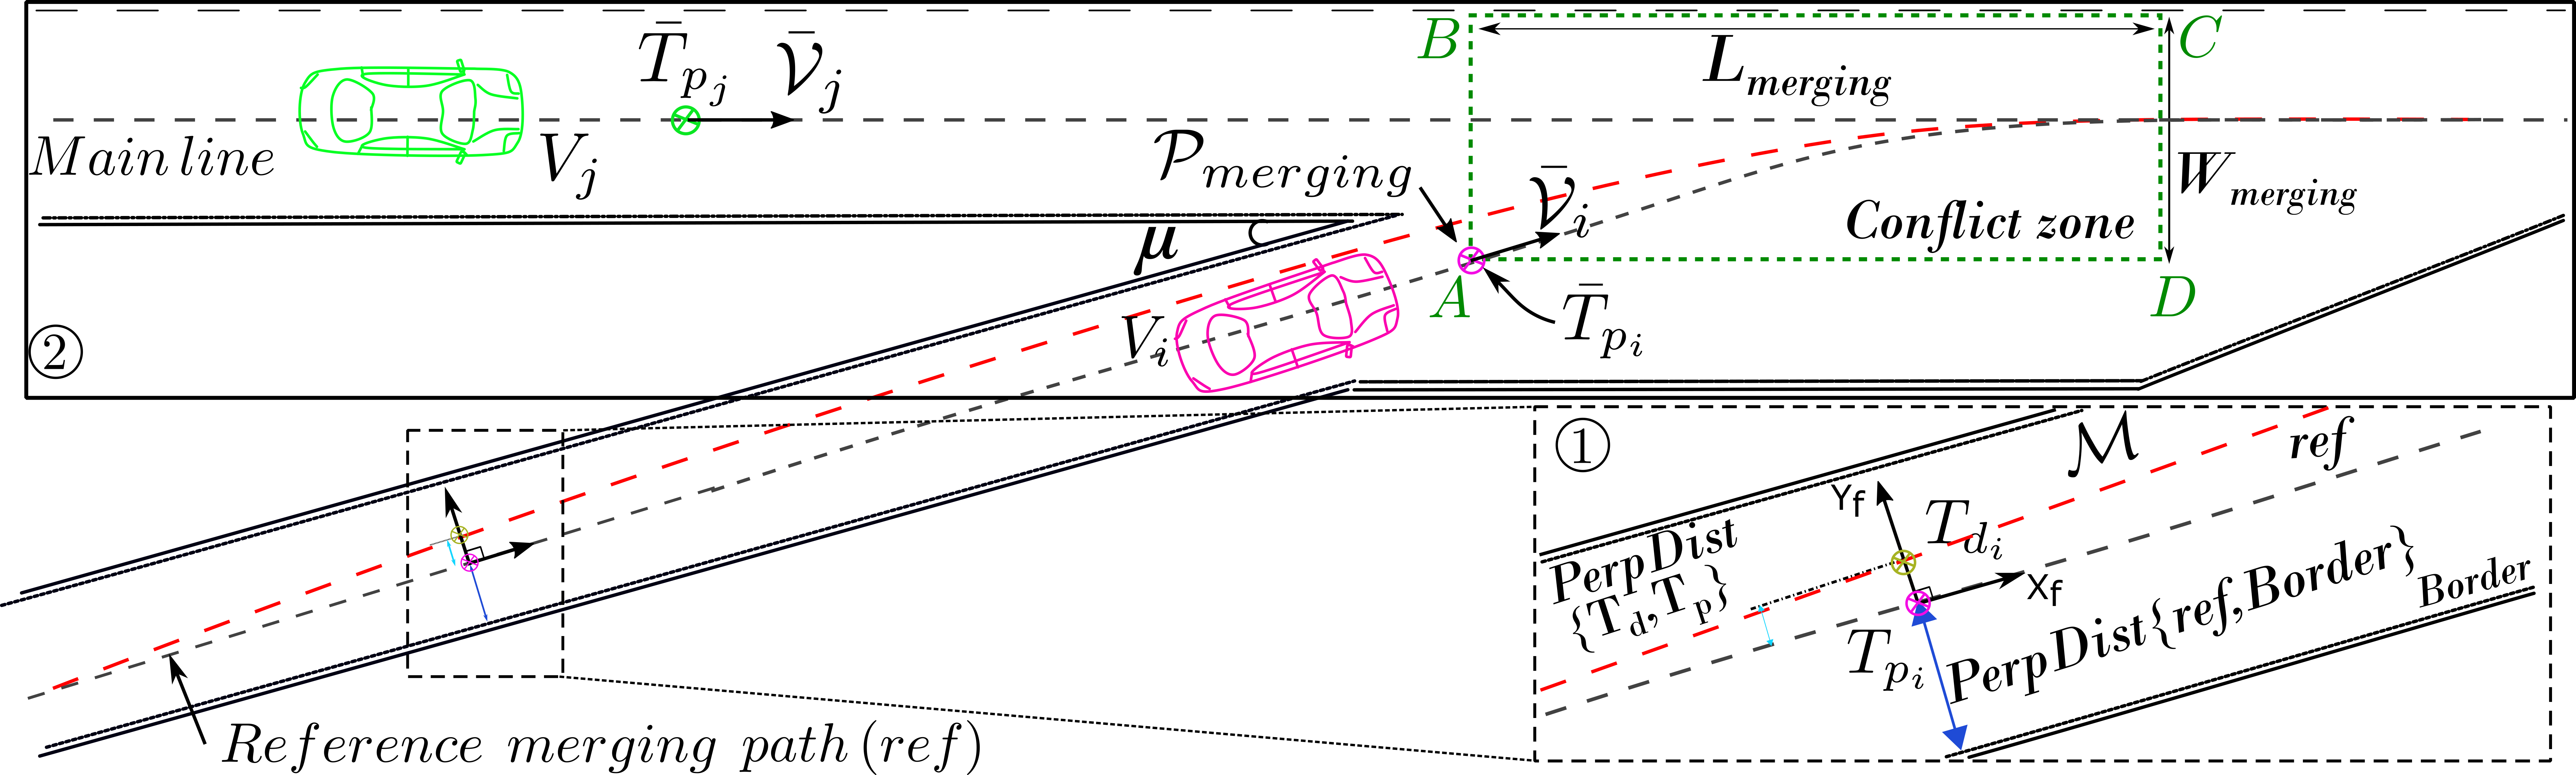
\includegraphics[width=12cm,height=5cm]{chapters/Chapitre_5/Figures/ScenarioMerging.png}
        %\vspace{-2.3mm}
        \caption{The projection of $T_{d_i}$ w.r.t. the reference trajectory}
        \label{fig:CORM-approximation}
        %\vspace{-5mm}
        \end{figure}




\tikzstyle{decision} = [diamond, draw, fill=white!,
    text width=2.5em, text badly centered, node distance=1.8cm, inner sep=1pt]
\tikzstyle{block} = [rectangle, draw, fill=white!,
    text width=20 em, text centered, minimum height=4em]
\tikzstyle{line} = [draw, very thick, color=black, -latex']
\tikzstyle{cloud} = [draw, ellipse, fill=white!, node distance=1.2cm,
    minimum height=2em]
\begin{figure}[!h]
\begin{center}
    \begin{tikzpicture}[scale=2, node distance = 1.2cm, auto]
    % Place nodes
    \tikzstyle{bigbox} = [minimum width=24em,draw=blue!50, thick, fill=blue!10, rounded corners, rectangle]
    \tikzstyle{bigbox2} = [minimum width=24em,draw=green!50, thick, fill=green!10, rounded corners, rectangle]

    \node [cloud] (n1) {\footnotesize Begin}; 
    \node [block, below of= n1,minimum height=1em,  minimum width=18em ,node distance= 0.9cm] (n2){\footnotesize{ Initialize optimization  parameters (cf. Algorithm \ref{alg: optimization algorithm})}};
    \node[block, below of= n2, minimum height=1em, minimum width=10em](n3){\footnotesize Fix gains $a_{i}$ and $a_j$ with $i \neq j $, $\forall i,j\in {N}$}; 
    \node[block, below of= n3, minimum height=1em, minimum width=10em](n4){\footnotesize Compute gains $a_{ij}$  with $i\neq j$ and $\forall i,j\in {N}$}; 
    \node[block, below of= n4, minimum height=1em, minimum width=10em](n5){\footnotesize Launch reconfiguration scenario}; 
    \node[block, below of= n5, minimum height=1em, minimum width=10em,node distance= 0.8cm](n6){\footnotesize Compute the value of the global objective function};
    \node[decision, below of= n6,minimum height=1em, minimum width=8em,node distance= 1.75cm ] (n7) {\footnotesize Reached stop criterion}; 
    \node[block, below of= n7, minimum height=1em, minimum width=20em,node distance= 6em](n8){\footnotesize Initialize reconfiguration scenario with $a_i^*,a_j^*$ and $a_{ij}^* $ with $i \neq j $, $\forall i,j\in {N}$}; 
    \node[block, below of= n8,minimum height=1em, minimum width=10em, node distance= 1cm](n9){\footnotesize Launch reconfiguration scenario}; 
    \node[block, below of= n9, minimum height=1em, minimum width=10em,node distance= 0.8cm](n10){\footnotesize Compute $t_{init}$, $t_{end}$ and traveled distance};         
    \node[block, below of= n10, minimum height=1em, minimum width=10em,node distance= 1cm](n11){\footnotesize Compute mean velocity $\bar{\mathcal{V}}_{i,j}$, $\forall i,j \in  {N}$ (cf. Algorithm \ref{alg: projection and computation of the mean velocity }, line 13)}; 
    \node[cloud, below of= n11,node distance= 1.1cm] (n12){\footnotesize End};  

    % Draw edges 
    \path[line] (n1)--(n2)node[text width=23.5em,text height=0em]{ \textcircled{\small{1}}}; 
    \path[line] (n2)--(n3); 
    \path[line] (n3)--(n4); 
    \path[line] (n4)--(n5); 
    \path[line] (n5)--(n6); 
    \path[line] (n6)--(n7); 
    \path[line] (n7.west) node [text width=6em,text height=2em]{\footnotesize No} -|(-2,-1.05)   -- (n3.west) ;
    \path[line] (n7)node [text width=4em,text height=8em]{\footnotesize Yes}--(n8); 
    \path[line] (n8)--(n9); 
    \path[line] (n9)--(n10); 
    \path[line] (n10)--(n11); 
    \path[line] (n11)--(n12) node [text width=23.5em,text height=-10em]{ \textcircled{\small{2}}}; 
    \begin{pgfonlayer}{background}
    \node[bigbox] [fit = (n2) (n7)] {};
    \node[bigbox2] [fit = (n8) (n12)] {};

   \end{pgfonlayer}
\end{tikzpicture}
\end{center}
%\vspace{-4mm}
\caption{The proposed CORM (Constrained Optimal Reconfiguration Matrix) flowchart. \numcircledmod{1} The optimization algorithm. \numcircledmod{2} The projection and mean velocity computation}
\label{fig:CormAlgo}
%\vspace{-5mm}%Put here to reduce too much white space after your table 

\end{figure} 
















In Figure \ref{fig:CormAlgo}, the details of the optimization process are illustrated. Following eq. \ref{eq:costfunction}, through the optimization algorithm based on gradient descent, it is aimed to compute the diagonal gains of the reconfiguration matrix $A$. The objective function is non-linear, the optimization algorithm (cf. Algorithm \ref{alg: optimization algorithm}, inputs) needs the optimization boundaries $[{a}_{i,j_{min}}, {a}_{i,j_{max}}]^T$  and the starting point $[a_{i_0}, a_{j_0}]^T$ with $i \neq j $, $\forall i,j\in {N}$. The anti-diagonal gains of $A$, in charge of the inter-target distances, are computed while using eq. \ref{eq:FinalDistaneStudy_2}. 

The full merging scenario is launched with a constant reconfiguration matrix $A$. The data related to the merging scenario are used to compute the objective function in eq. \ref{eq:costfunction} (cf. Algorithm \ref{alg: optimization algorithm}). The latter is used to judge on the stop criterion; when the minimum of the cost function is reached. At last, the optimization algorithm returns the optimal values of the gains $a_i^*$ and $a_j^*$, $i \neq j $, $\forall i,j\in {N}$, the gains $a_{ij}, i\neq j,  i,j\in {N}$ are computed with the help of eq. \ref{eq:FinalDistaneStudy_2}.




\begin{algorithm}
\begin{small}
\DontPrintSemicolon
\SetKwInOut{Input}{Input}
\SetKwInOut{Output}{Output}
\SetKwInOut{Variables}{Variables}
\SetKwInOut{Parameters}{Parameters}
\Input{$GlobalInput$  Scenario data \\$[{a}_{i_{min}}, {a}_{i_{max}}]^T$ boundaries of the gain $a_i$ \\
$[{a}_{j_{min}}, {a}_{j_{max}}]^T$ boundaries of the gain $a_j$ \\ $[{a_{i_{0}}}, {a_{j_{0}}}]^T$start point of the optimization \\
$ObjectiveFunction$ the objective function in eq. \ref{eq:costfunction}}% an intervention}


\Output{$[a_i^*,a_j^*]^T $ optimal values of the gains $a_i$ and $a_j$ } 
$MergingData \leftarrow [PerpDist\{T_{d_{i}}, {T}_{p_{i}}\},PerpDist\{T_{d_{j}}, {T}_{p_j}\},$
$ PerpDist\{{T}_{p_i}, Border\}, PerpDist\{{T}_{p_j}, Border\}]^T $\;
\While{$(StopCriterion \neq True)$}
{
  %\tcp*[l]{next intervention of ordered list of interventions to be scheduled }
  $[a_{i}, a_{j}]^T \leftarrow Fixe([{a_{i_{0}}}, {a_{j_{0}}}]^T, [{a}_{i}_{min}, {a}_{i}_{max}]^T,[{a}_{j}_{min}, {a}_{j}_{max}]^T )$\; 
   $MergingData \leftarrow MergingScenario(GlobalInput, a_i, a_j) $\; 
  %\tcp*[l]{select modes and time intervals for intervention $p$}
  %\tcp*[l]{assess cost}
  $T \leftarrow length(MergingData)$ \;
  \ForAll{$t \in [0, T]$}
  {
    $Cost(t) \leftarrow ObjectiveFunction(MergingData(t)) $
  }
  $GlobalCost \leftarrow Sum(Cost)$
  
}
%\Return $S_i, \mathcal{L}_{u}$\;
\caption{Optimization Algorithm}\label{alg: optimization algorithm}
\end{small}

\end{algorithm}


\subsubsection{Safe and feasible local trajectory planning}  \label{sec:Projected_target}

In this section it is proposed to delve into the projection approach based on a Frenet reference frame that ensures the respect of the global reference path imposed by the global reference planner. In addition, this section presents the computation of the velocity profile imposed to the projected target $T_p$ to ensure the safety, feasibility, and smoothness of the merging maneuver. 

\begin{enumerate}
    \item \textbf{\textit{Global reference aware target:}} The constrained optimal inter-target distance matrix allows to respect the road constraints while ensuring the vehicle's safety. However, the generated targets $T_d$ are not guaranteed to be onto the reference path (cf. Figure \ref{fig:CORM-approximation} \numcircledmod{1}). In order to ensure this requirement, it is proposed to use the reference path as a guiding system for the vehicle and compute its effective target $T_p$ w.r.t. this latter (cf. Figure \ref{fig:CORM-approximation} \numcircledmod{1}).

    Each target $T_d$ of the merging vehicle is projected w.r.t. the reference merging path using a Frenet reference frame $[X_f,Y_f]$ (cf. Figure \ref{fig:CORM-approximation}) to obtain $T_p$. The lines 10 and 11 in Algorithm \ref{alg: projection and computation of the mean velocity } and eq. \ref{eq:frenetToCartisian} details the transformation from the mobile reference frame centered on $V_R$ to the global reference frame $[X_G,Y_G]$, in addition to the projection function that uses the reference merging path and $T_d \in \mathcal{M}$ to obtain $T_p$ (cf. Figure \ref{fig:CORM-approximation} \numcircledmod{1})


    \item \textbf{\textit{Safe and feasible velocity profile:}} The projected target $T_p$ has a similar dynamic as $T_d$. However, in order to draw full advantage from the constrained optimal inter-target distance matrix in terms of safety formal insurance, it is proposed to use the latter to compute the necessary mean velocity that must be imposed to the vehicles, such that they enter the conflicting zone in Figure \ref{fig:CORM-approximation} \numcircledmod{2} at the same moment as if they have followed $T_d$. 

    Before the presentation of the details related to the imposed dynamics, for the clarity and the understanding of the reader, it is proposed to define the conflicting zone. The conflicting zone in  Figure \ref{fig:CORM-approximation} \numcircledmod{2} defines the area where a collision between the merging vehicle and the vehicle on the highway vehicle may occur. $\mathcal{P}_{merging}$ defines the position of the merging vehicle where the surrounding circles of $V_i$ and $V_j$ may overlap, resulting in a collision. The points $A$, $B$, $C$, and $D$ define the limits of the conflicting zone. $A$ is the pose of the merging vehicle where a collision may occur, $B$ is related to the limits of the merging zone, $D$ defines the end of the merging zone, while $C$ is its projection w.r.t. the highway center-line (cf. Figure \ref{fig:CORM-approximation} \numcircledmod{2}). 


\begin{algorithm}
\begin{small}
\DontPrintSemicolon
\SetKwInOut{Input}{Input}
\SetKwInOut{Output}{Output}
\SetKwInOut{Variables}{Variables}
\SetKwInOut{Parameters}{Parameters}
\Input{$GlobalInput$  Scenario data \\  $a_i^* , a_j^*, a_{ij}^*$ optimal gains of the reconfiguration matrix (cf. Algorithm \ref{alg: optimization algorithm})} % an intervention}


\Output{$\widebar{\mathcal V}_{i,j}$ the mean velocity of the vehicles $V_i$ and $V_j$}

%\Variables{$\mathcal{S}_{p,sr(ti)c}$ for intervention $p$, \\
%\hspace{35pt} set of quadruplets (\textbf{s}urgeon, \textbf{r}oom, 
%\textbf{t}ime \textbf{i}nterval, \textbf{c}ost)}
%\vspace{5pt}
%$\mathcal{L}_{u} \leftarrow \emptyset$ \;
$k \leftarrow 1$ \; 
$\mathcal{F}(k) \leftarrow {F^{init}}$\; 
$\varepsilon (k) \leftarrow  \mathcal{F}^{end}-\mathcal{F}(k)$\; 
$ Buffer_R \leftarrow ReferenceTrajectory(V_R)$\;
$ Buffer_{i,j} \leftarrow ReferenceTrajectory(V_i,V_j)$\;

\While{$(\varepsilon (k)\neq 0)$}
{
  $k \leftarrow k+1$ \; 
  %\tcp*[l]{next intervention of ordered list of interventions to be scheduled }
  $\mathcal{F} (k) \leftarrow DynamicReconfiguration ( \mathcal{F}^{end},\mathcal{F}(k-1)) $\;
  $\varepsilon (k) \leftarrow  \mathcal{F}^{end}-\mathcal{F}(k)$\; 
  %\tcp*[l]{select modes and time intervals for intervention $p$}
  %\tcp*[l]{assess cost}
  $T_{d_{i,j}}(k) \leftarrow Transform(Buffer_R,\mathcal{F}(k), X_{V_{R}})  $ \;
  ${T}_{p_{i,j}}(k) \leftarrow Projection(Buffer_{i,j},{T}_{d_{i,j}})  $ \;
  $X_{V_{i,j}} (k)  \leftarrow Control(X_{V_{i,j}} (k-1),{T}_{p_{i,j}}(k))$\; 
  }
  $\widebar{\mathcal V}_{i,j}= \frac{CurviDist \{V_{i,j}(1,k)\}}{t_{end}-t_{init}}$\;
 
%\Return $S_i, \mathcal{L}_{u}$\;
\caption{\small Projections and computation of the imposed dynamic \label{alg: projection and computation of the mean velocity }}
\end{small}
\end{algorithm}




    Based on the definition of the conflicting zone, it is proposed to compute the mean velocity $\bar{\mathcal{V}}_{i,j}$ where $i,j$ are the indices of the vehicles $V_i$ and $V_j$ respectively (cf. Figure \ref{fig:CORM-approximation} \numcircledmod{2}), such that the in-between distance respects the following:  
\begin{align}
    EucDist \{\bar{T}_{p_j}(t_{end}),\bar{T}_{p_i}(t_{end})\}= 
    EucDist \{T_{d_j}(t_{end}),T_{d_i}(t_{end})\}
\end{align}

where $t_{end}$ is the time when the pose $\mathcal{P}_{merging}$ (cf. Figure \ref{fig:CORM-approximation}) is reached by the merging vehicle. $EucDist \{T_{d_j}(t_{end}),{T}_{d_i}(t_{end})\}$  represents the Euclidean distance between the targets $T_{d_{i}}$ and $T_{d_j}$ generated during the first step of the proposed CORM for the vehicles $V_i$ and $V_j$, while $EucDist \{\bar{T}_{p_j}(t_{end}),\bar{T}_{p_i}(t_{end})\}$ (Figure \ref{fig:CORM-approximation} \numcircledmod{2}) is the in-between Euclidean distance between the targets with the imposed dynamic $\bar{\mathcal{V}}_{i}$  and  $\bar{\mathcal{V}}_{j}$ for the vehicles $V_i$ and $V_j$, respectively.  



The mean velocity $\bar{\mathcal{V}}_{i,j}$ where $i,j$ are the indices of the vehicles $V_i$ and $V_j$ (Figure \ref{fig:CORM-approximation} \numcircledmod{2}) is computed based on the line 13 in Algorithm \ref{alg: projection and computation of the mean velocity }, where $t_{init}$ is the corresponding time when the reconfiguration was launched. A curvilinear distance formula is used to get the traveled distance by each vehicle between $t_{init}$ and $t_{end}$. 




In order to have the smoothest possible behavior w.r.t. the vehicles' dynamics, it is proposed to use a sigmoid function to shape the velocity profile. This latter is used to create a velocity profile that goes from the vehicle initial velocity toward the mean velocity, and goes to the reference vehicle $V_R$ velocity when the vehicle enters the main line. This choice is motivated by the sigmoid ability to smoothly control the convergence rate from an initial velocity to the final desired one. In other terms, using the sigmoid function permits us to impose a feasible and comfortable acceleration and deceleration profile to the vehicles. 








    
\end{enumerate}


\subsection{Simulation results}\label{sec:CORM_simulation}

In order to evaluate the efficiency of the CORM in terms of its ability to guarantee the safety requirement as well as the smoothness of the vehicle's dynamics, while performing the on-ramp merging maneuver, a first scenario is proposed. It aims to perform the merging maneuver with a formation of three vehicles. The simulation video can be found in \textcolor{blue}{https://youtu.be/UM2cLt74pVM}. Then, a comprehensive summary of several conducted simulations is presented in Table \ref{Tab: Summary}. 

\begin{enumerate}
    \item \textbf{\textit{On-ramp merging in formation:}} 
    
        \begin{figure}[!h]
        \centering 
        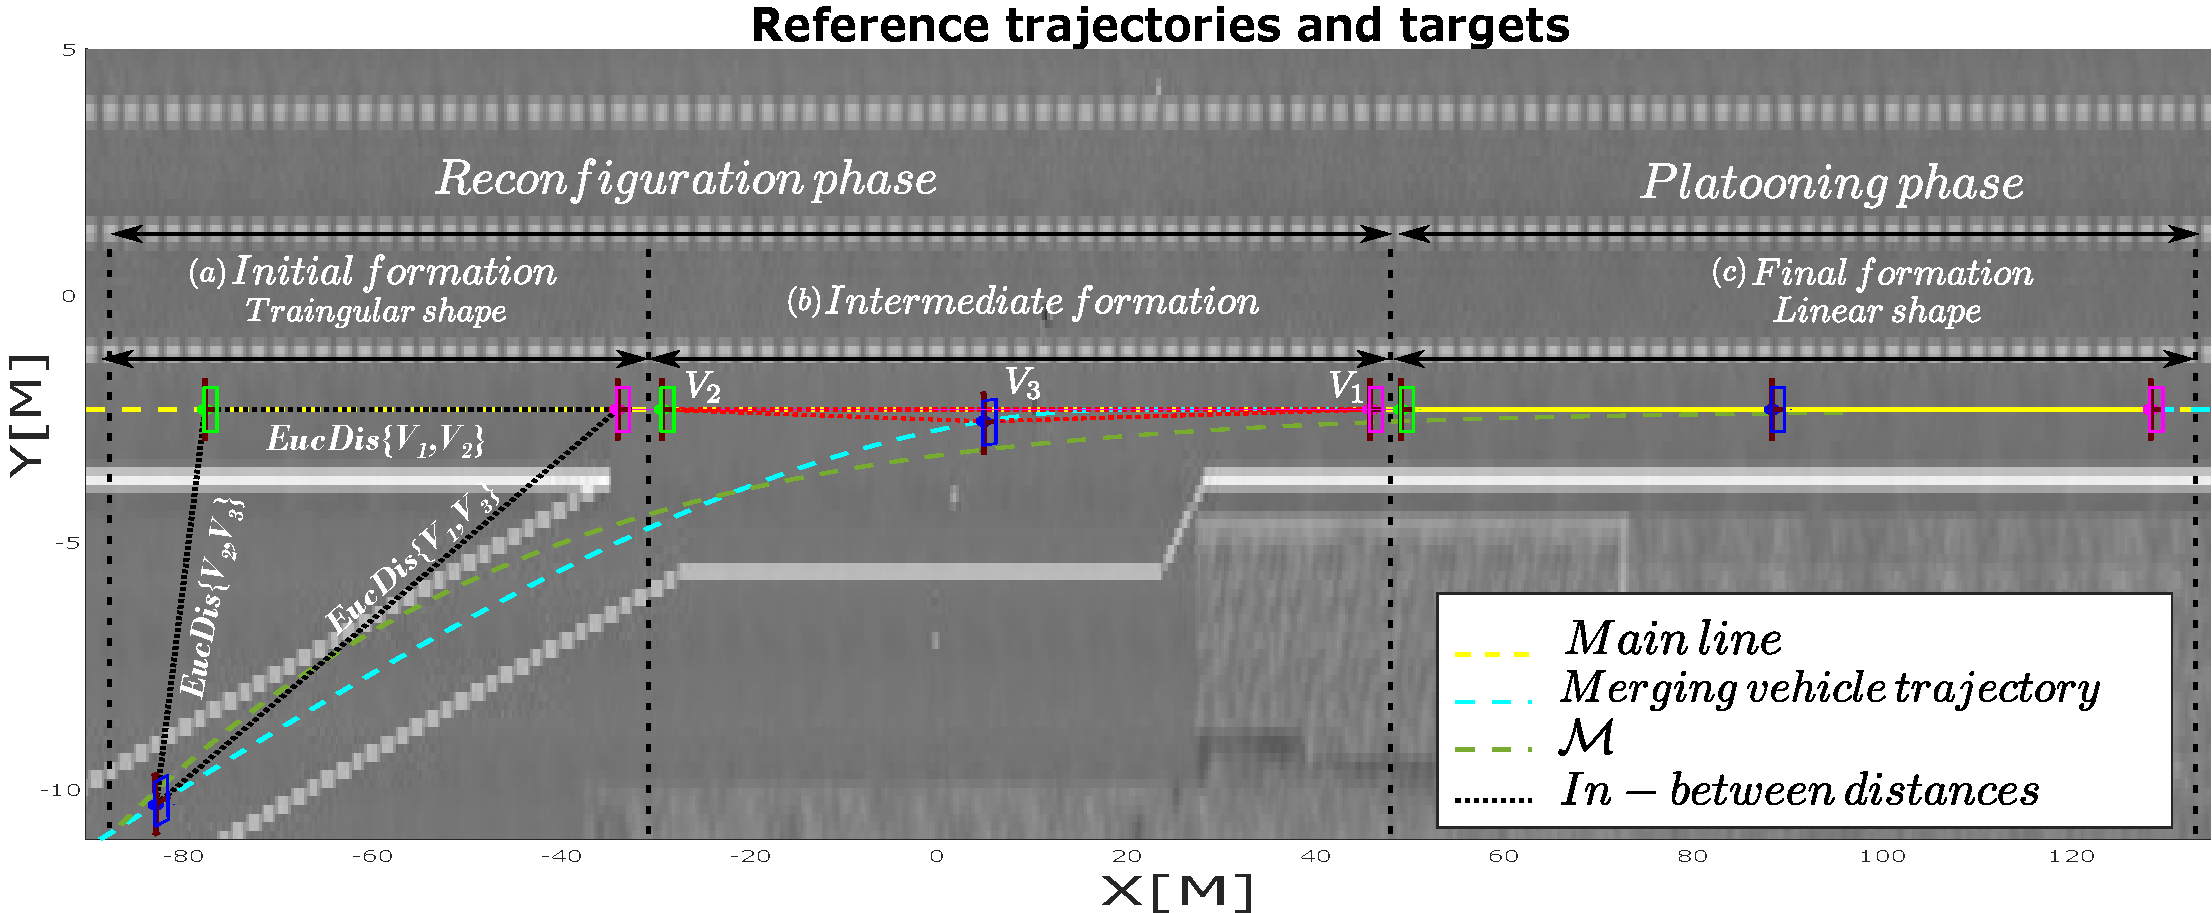
\includegraphics[width=14cm,height=18cm,keepaspectratio]{chapters/Chapitre_5/Figures/CORM/MergingSimulation.pdf}
        %\vspace{-2.3mm}
        \caption{Evolution of the formation shape during the merging performed by the CORM framework (\textcolor{blue}{Simulation video: https://youtu.be/UM2cLt74pVM})}
        \label{fig:CORM: formation_shape}
        %\vspace{-5mm}
        \end{figure}

    In the following simulation, it is aimed to perform a merging maneuver with a formation of three vehicles. The considered merging scenario is an on-ramp merging with an incidence angle $\mu=10^\circ $, $V_1$ (i.e., the reference vehicle $V_R$) is placed in the main line, so as $V_2$. The third vehicle $V_3$ initially placed in the secondary on-ramp merging road (cf. Figure \ref{fig:CORM: formation_shape}). The initial formation shape is triangular (cf. Figure \ref{fig:CORM: formation_shape}), consequently at the end of the reconfiguration phase the aim is to put the vehicles part of the formation in a linear shape to form a platoon (cf. Figure \ref{fig:CORM: formation_shape}). Table \ref{Tab: inputs} resumes the scenario inputs. 

\begin{table}[]
%\scriptsize
\begin{center}
\caption{The values of the inputs of the CORM algorithm}

\label{Tab: inputs}

\begin{tabular}{lll}

\cline{1-2}  
\multicolumn{1}{|l|}{Inputs}                                    & \multicolumn{1}{l|}{Values}                                                                                                                              &  \\ \cline{1-2}                 
\multicolumn{1}{|l|}{Initial formation coordinates $[m]$}       & \multicolumn{1}{l|}{\begin{tabular}[c]{@{}l@{}}$\left (\begin{smallmatrix}\\   0 & -40 &-50 \\\\   0 &0& 9.2 \\  \end{smallmatrix}\right)$\end{tabular}} &  \\ \cline{1-2}
\multicolumn{1}{|l|}{Final formation coordinates $[m]$} & \multicolumn{1}{l|}{\begin{tabular}[c]{@{}l@{}}$\left(\begin{smallmatrix}\\ 0 &-80&-40\\\\ 0&0&0\\ \end{smallmatrix}\right)$\end{tabular}}                                    &  \\ \cline{1-2}
\multicolumn{1}{|l|}{$\mathcal{V}_{1,2,3}[m/s]$}                & \multicolumn{1}{l|}{$[19.4, 19.4,19.4]$}                                                                                                              &  \\ \cline{1-2}
\multicolumn{1}{|l|}{$[{a}_2_{min}, {a}_2_{max}]^T$}     & \multicolumn{1}{l|}{$[-0.4, 0.1]$}                                                                                                                     &  \\ \cline{1-2}
\multicolumn{1}{|l|}{$[{a}_3_{min}, {a}_3_{max}]^T$}     & \multicolumn{1}{l|}{$[-0.4, -0.05]$}                                                                                                                   &  \\ \cline{1-2}
\multicolumn{1}{|l|}{$[a_{2_{0}}, a_{3_{0}}]^T$}                & \multicolumn{1}{l|}{$[-0.25, -0.25]$}                                                                                                                  &  \\ \cline{1-2}
\multicolumn{1}{|l|}{$[w_2, w_3]^T$}                  & \multicolumn{1}{l|}{$[1, 4]$}                                                                                                                          &  \\ \cline{1-2}
\multicolumn{1}{|l|}{$[a_{2}^*, a_{3}^*]^T$}                    & \multicolumn{1}{l|}{$[-0.1228, -0.365]$}                                                                                                               &  \\ \cline{1-2}
\multicolumn{1}{|l|}{$\underline{D}_T[m]$}                      & \multicolumn{1}{l|}{$12$}                                                                                                                                &  \\ \cline{1-2}
                                                                &                                                                                                                                                          & 
\end{tabular}
\end{center}
\vspace{-10mm}%Put here to reduce too much white space after your table 
\end{table}


    

    The minimum inter-target distance $\underline{D}_T$ (cf. Figure \ref{fig:safetydistance}) is computed using the following model: 
    \begin{equation} \label{eq:minimum_distance_model}
    \underline{D}_T= (R_i + R_j)  + offset
    \end{equation}

    where $R_i$ and $R_j$ are the radius of the circles that surround the vehicles $V_i$ and $V_j$, and $offset$ is the safety distance to avoid rear-end collisions. 











The reconfiguration of the triangular shape toward the desired linear one is illustrated in Figure \ref{fig:CORM: formation_shape}. The formation defined by its initial coordinates passes through the reconfiguration phase, where $V_3$ is in front of $V_2$ as desired w.r.t. the formation's final coordinates, consequently, the $EucDist(V_1,V_2)$ needs to increase. The intermediate formation showcases the pose of the three vehicles in the conflict zone. As expected $EucDist(V_1,V_2)$ has increased to make space for $V_3$ in the convoy. In the second phase, after the convergence of the formation toward its desired shape, the vehicles form a linear shape, where the desired in-between distances are respected. 

        \begin{figure}[!h]
        \centering 
        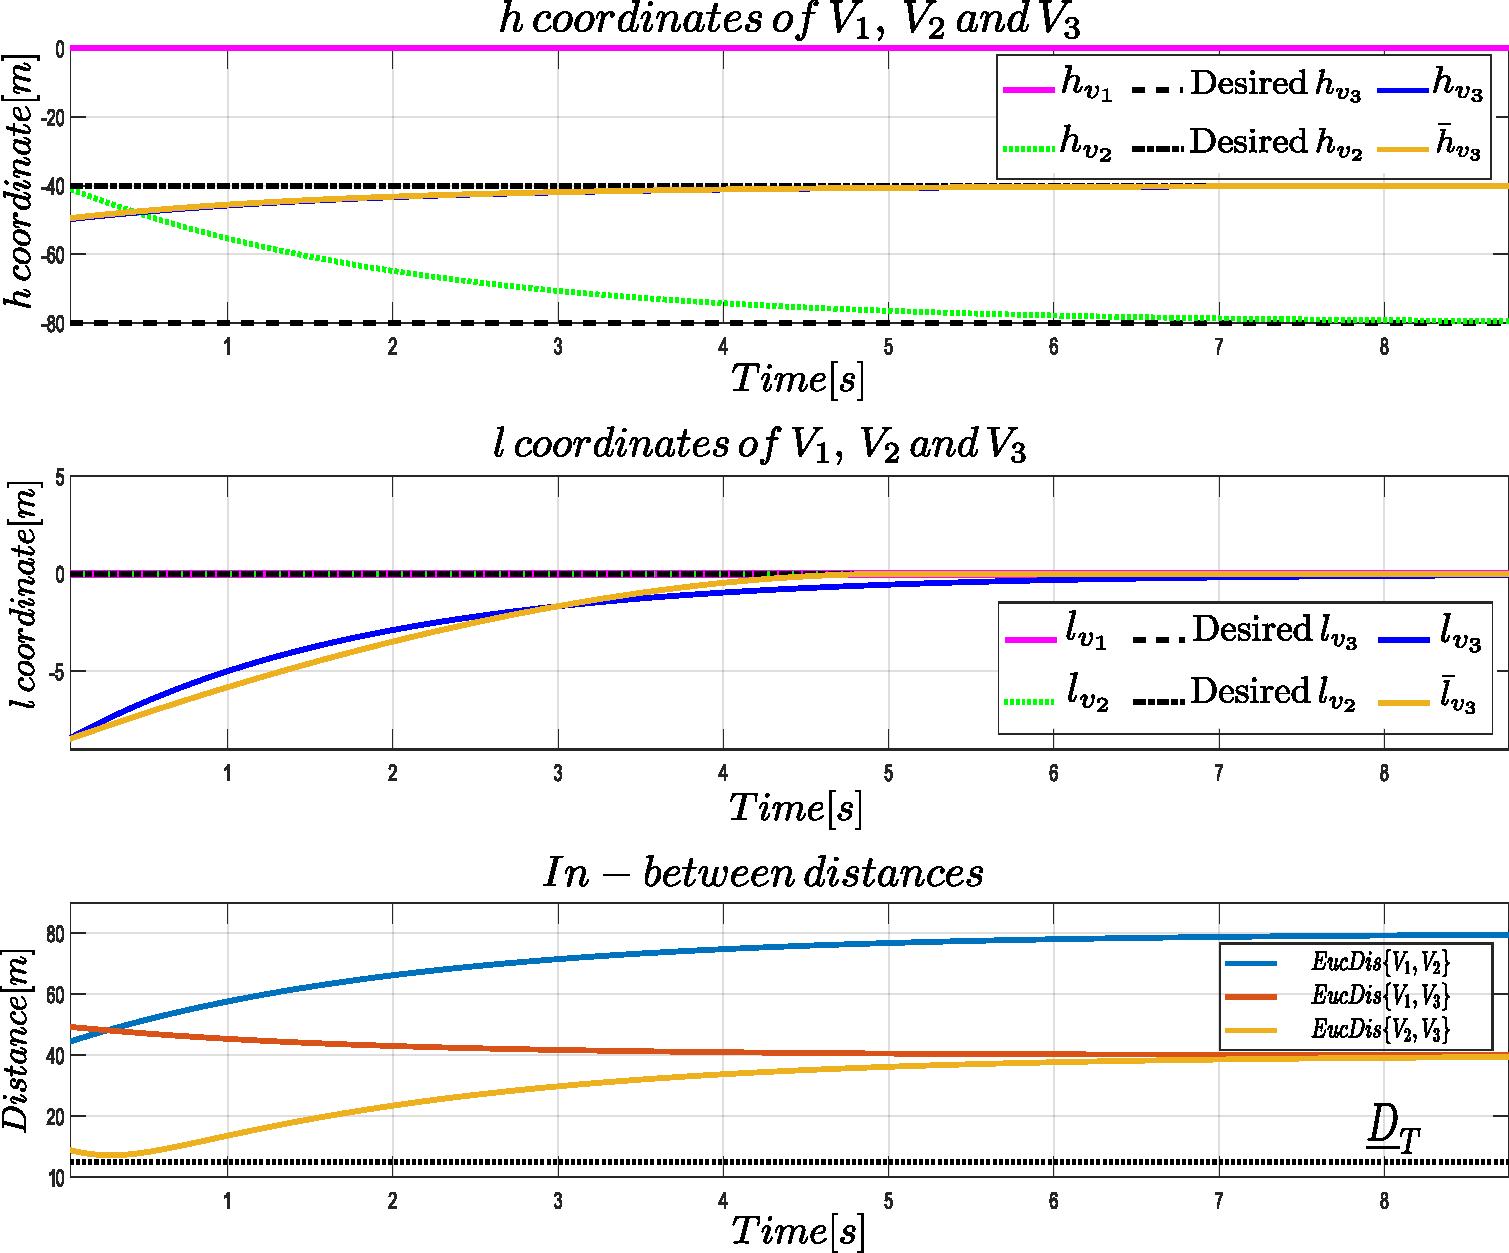
\includegraphics[width=11cm,height=18cm,keepaspectratio]{chapters/Chapitre_5/Figures/CORM/In_between_distances.pdf}
        %\vspace{-2.3mm}
        \caption{The formation coordinates and the Euclidean in-between distances profiles}
        \label{fig:CORM: formation_coordinates}
        %\vspace{-5mm}
        \end{figure}

To evaluate the CORM capability in terms of safety and convergence errors, it is proposed to study the evolution of the formation coordinates and the in-between distances profiles illustrated in Figure \ref{fig:CORM: formation_coordinates}. A first order asymptotic convergence from the initial formation shape toward the desired one can be noticed in the formation coordinates plots. As for the minimum distances, the in-between distances profiles are always greater than $\underline{D}_T$. The in-between distances when the vehicles are in the conflicting zone is greater than  $20m$. The final in-between distances meet the safety requirement for a convoy formation; $EucDist(V_i, V_j)=2[s]\times \mathcal{V}_{i,j}[m/s]=40m$. 


        \begin{figure}[!h]
        \centering 
        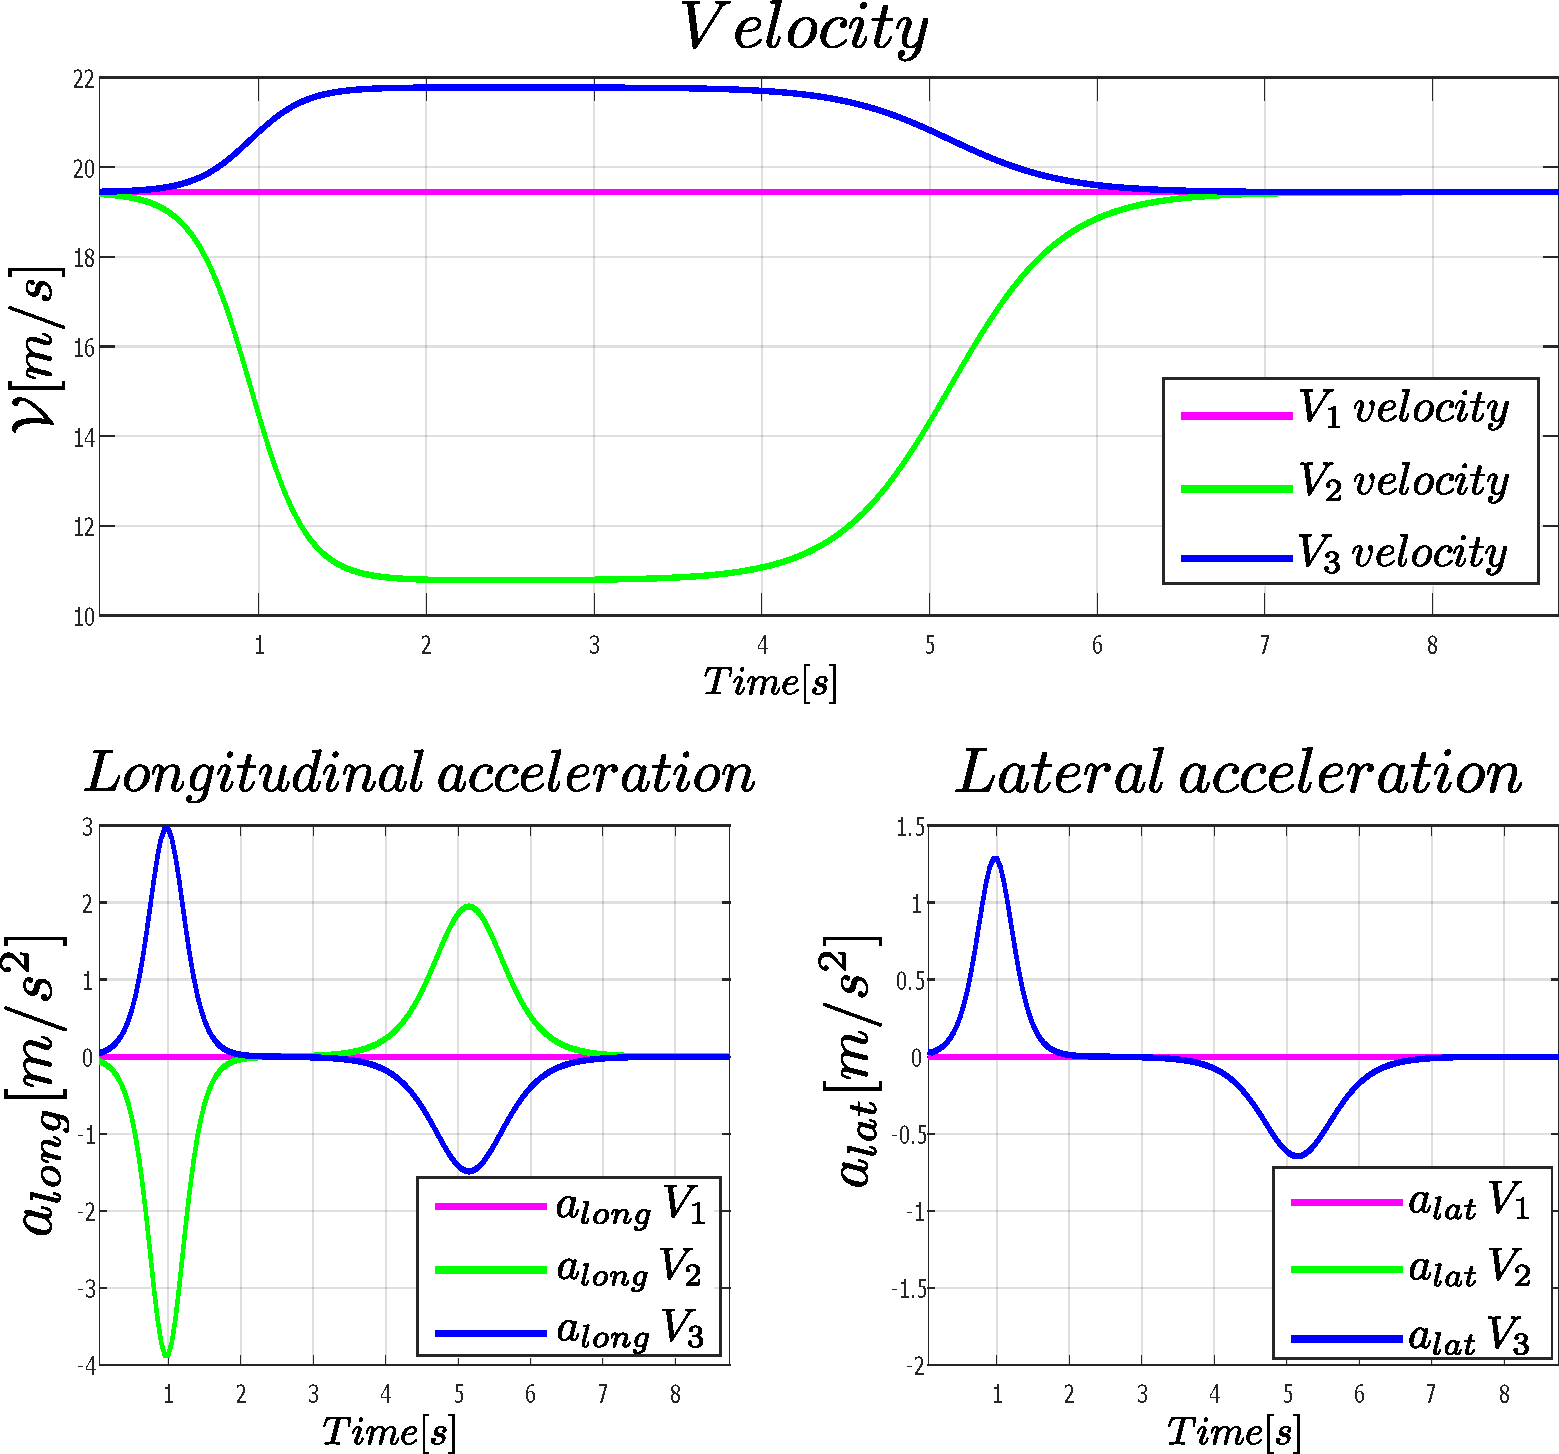
\includegraphics[width=10cm,height=18cm,keepaspectratio]{chapters/Chapitre_5/Figures/CORM/velocities.pdf}
        %\vspace{-2.3mm}
        \caption{The vehicles' velocity and acceleration profiles}
        \label{fig:CORM: velocity}
        %\vspace{-5mm}
        \end{figure}





In Figure \ref{fig:CORM: velocity}, the linear velocity, the longitudinal, and the lateral accelerations are presented for each of the three vehicles part of the formation. As expected, the velocity of the vehicle $V_2$ decreases at the beginning of the scenario to make space for $V_3$, before it increases to make sure that $V_2$ meets the velocity requirement in the platoon. As for $V_3$, its velocity increases at the beginning to enter the highway center-line while respecting the safety distances. A decreasing can be noticed around $4s$ to follow the convoy velocity (fixed to $19.4 m/s$ - $70 km/h$). Figure \ref{fig:CORM: velocity} confirms that the longitudinal and the lateral accelerations respect the maximum and minimum authorized accelerations (i.e., $-4m/s^2$ for deceleration and $3m/s^2$ for acceleration). Thus, with the help of the results in Figure \ref{fig:CORM: velocity}, the vehicles' dynamics during the formation reconfiguration while the merging is performed are smooth and comfortable. 




 \item \textbf{\textit{Influence of the projection phase on the CORM efficiency:}} 

 This section is dedicated to validate more intensively the proposed approach, while emphasizing mainly the ability of the projection phase for different environments structure (several values of $\mu$). 

        % \begin{figure}[!h]
        % \centering 
        % 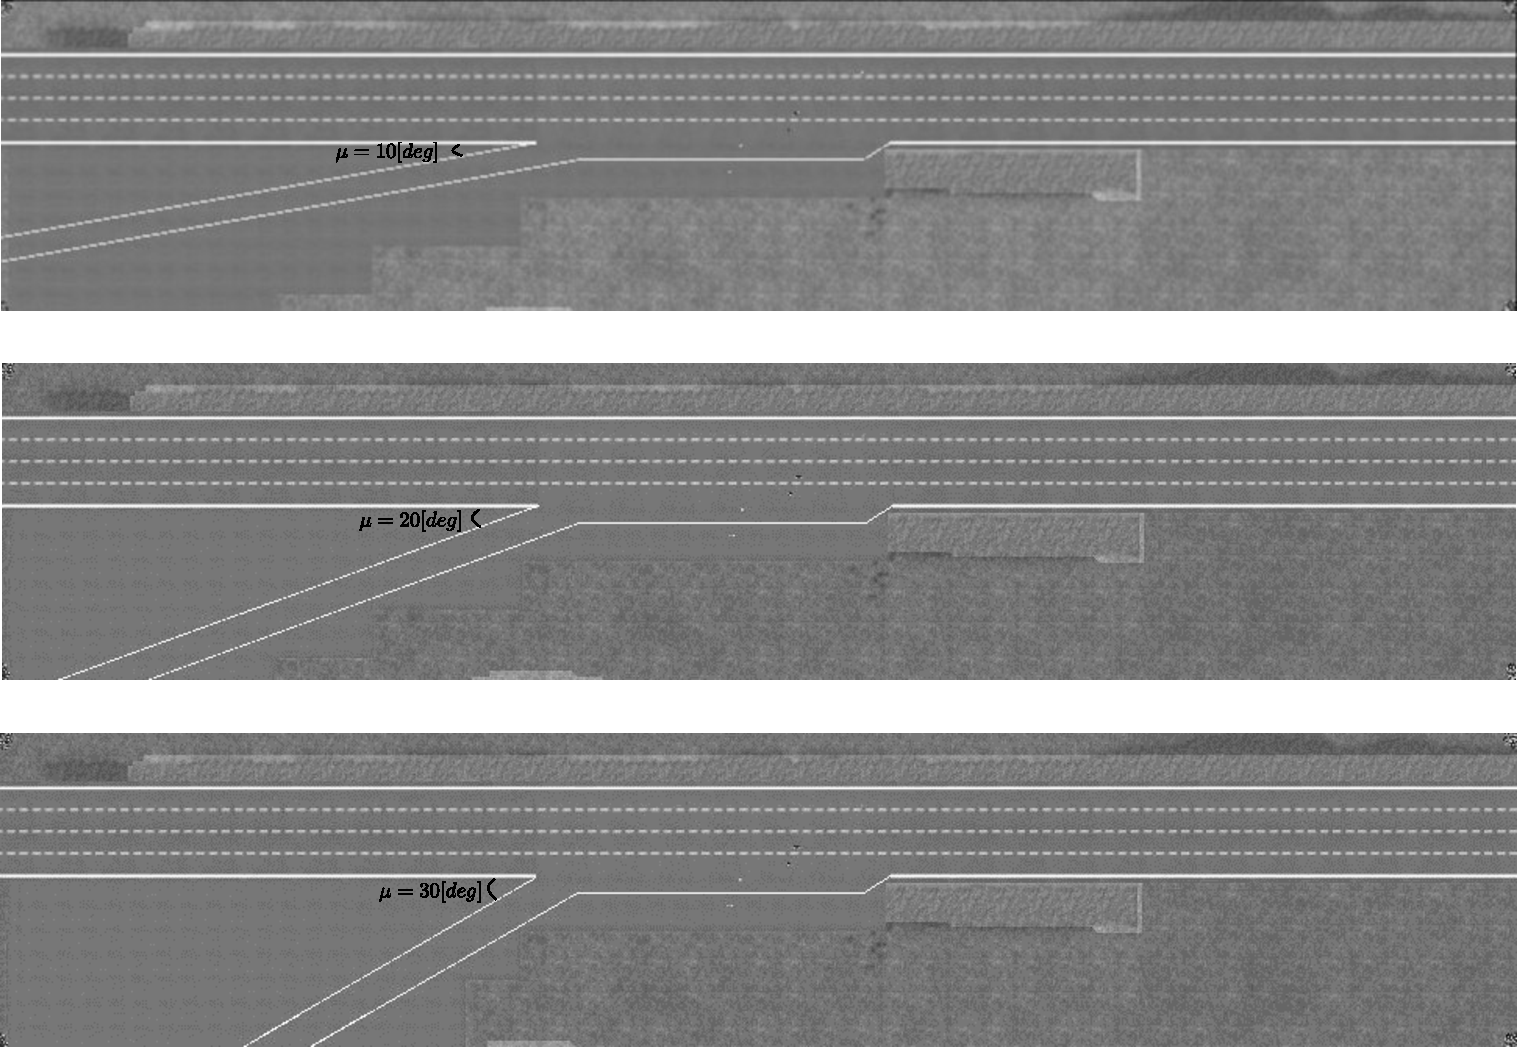
\includegraphics[width=10cm,height=18cm,keepaspectratio]{chapters/Chapitre_5/Figures/CORM/CORM_summary.pdf}
        % %\vspace{-2.3mm}
        % \caption{Range of incidence angles between $ \mu = 10^\circ$ and $\mu = 30^\circ$}
        % \label{fig:CORM: mu}
        % %\vspace{-5mm}
        % \end{figure}

 

For a range of incidence angles between $ \mu = 10^\circ$ and $\mu = 30^\circ$ with $\Delta \mu = 10^\circ$ step each time. It is proposed to study the performance of the CORM for velocity between $5 m/s$ and $15 m/s$ with an increase of $5 m/s$ each time. For all the simulations, the inputs of the CORM algorithm are the same as in Table \ref{Tab: inputs}. The conducted simulations are summarized in Table \ref{Tab: Summary}.



According to the performed simulations, it is important to emphasize that the safety of the vehicles is always ensured; the minimum inter-vehicle distance in the conflicting zone $\underline{D_{T}}$  is always greater than $20m$. The metric $Error_{max}$ is the maximum distance between $T_d$ and $\bar{T}_{p}$. This latter is lower than $1.5m$ (distance between the center-line and the road border), in other terms, $T_d$ is never out of the road borders. 

To evaluate the smoothness of the merging, it is proposed to discuss the obtained velocity and acceleration profiles w.r.t. variable velocity of the reference velocity and different incidence angles. The velocity profiles are similar to the one in Figure \ref{fig:CORM: velocity}, with a sigmoid shape that makes $\mathcal{V}_2$ decrease toward $\underline{\mathcal{V}}_2$ to make space for $V_3$, and $\mathcal{V}_3$ increase toward $\bar{\mathcal{V}}_3$ in the beginning. Then, $\mathcal{V}_2$ and $\mathcal{V}_3$ increases and decreases respectively toward $\mathcal{V}_R$ to form the final desired platoon. As for the acceleration, the lateral and the longitudinal behavior respect the limits of feasibility and comfort (i.e., $-4 m/s^2$ for the deceleration and $3m/s^2$ for the acceleration).
 



\newpage
\thispagestyle{empty}
\begin{landscape}
\begin{table*}[!h]
\setlength\tabcolsep{6.5pt} % default value: 6pt
%\scriptsize

\centering
\caption{The summary results of the conducted simulation for a variable incidence angle $\mu$ and vehicles' velocity $\mathcal{V}$ }
  %\centering
  %\captionsetup{singlelinecheck=off, skip =4pt}
  \begin{adjustwidth}{-0.235\textwidth}{-0.10\textwidth}
%\vspace{-2.3mm}
\label{Tab: Summary}

\begin{tabular}{|l|lll|lll|lll|}
\hline
$\mu[\deg]$                                                       & \multicolumn{3}{l|}{10}                                                                                            & \multicolumn{3}{l|}{20}                                                                                          & \multicolumn{3}{l|}{30}                                                                                     \\ \hline
$\mathcal{V}_{R}[m/s]$                                            & \multicolumn{1}{l|}{5}                     & \multicolumn{1}{l|}{10}                    & 15                       & \multicolumn{1}{l|}{5}                   & \multicolumn{1}{l|}{10}                    & 15                       & \multicolumn{1}{l|}{5}                    & \multicolumn{1}{l|}{10}                  & 15                   \\ \hline
$[\underline{\mathcal{V}}_{2}, \overline{\mathcal{V}}_{2}][m/s]$  & \multicolumn{1}{l|}{{[}4.36, 5{]}}       & \multicolumn{1}{l|}{{[}8.73,10{]}}      & {[}13.45, 15{]}        & \multicolumn{1}{l|}{{[}4.21, 5{]}}     & \multicolumn{1}{l|}{{[}8.49,10{]}}       & {[}13.26, 15{]}        & \multicolumn{1}{l|}{{[}4.13, 5{]}}      & \multicolumn{1}{l|}{{[}8.35,10{]}}     & {[}13.06,15{]}     \\ \hline
$[\underline{\mathcal{V}}_{3}, \overline{\mathcal{V}}_{3}][m/s]$ & \multicolumn{1}{l|}{{[}5,5.59{]}}       & \multicolumn{1}{l|}{{[}10,11.125{]}}      & {[}15,16.80{]}         & \multicolumn{1}{l|}{{[}5,5.824{]}}       & \multicolumn{1}{l|}{{[}10,11.6316{]}}      & {[}15,17.43{]}           & \multicolumn{1}{l|}{{[}5,6.10{]}}       & \multicolumn{1}{l|}{{[}10,12.10{]}}    & {[}15,18.14{]}     \\ \hline
$[\underline{a}_2,\overline{a}_2]_{long}[m/s^2]$                  & \multicolumn{1}{l|}{{[}-0.29, 0.15{]}} & \multicolumn{1}{l|}{{[}-0.60, 0.29{]}} & {[}-0.70, 0.35{]}{]} & \multicolumn{1}{l|}{{[}-0.35, 0.18{]}}  & \multicolumn{1}{l|}{{[}-0.68, 0.34{]}} & {[}-0.78, 0.53{]} & \multicolumn{1}{l|}{{[}-0.38,0.19{]}} & \multicolumn{1}{l|}{{[}0.70,0.37{]}}  & {[}-0.87,0.44{]} \\ \hline
$[\underline{a}_2,\overline{a}_2]_{lat}[m/s^2]$                   & \multicolumn{1}{l|}{{[}0,0{]}}             & \multicolumn{1}{l|}{{[}0,0{]}}             & {[}0,0{]}                & \multicolumn{1}{l|}{{[}0,0{]}}           & \multicolumn{1}{l|}{{[}0,0{]}}             & {[}0,0{]}                & \multicolumn{1}{l|}{{[}0,0{]}}            & \multicolumn{1}{l|}{{[}0,0{]}}           & {[}0,0{]}            \\ \hline
$[\underline{a}_3,\overline{a}_3]_{long}[m/s^2]$                  & \multicolumn{1}{l|}{{[}-0.76,1.52{]}}  & \multicolumn{1}{l|}{{[}-1.66, 2.02{]}}    & {[}-1.14,2.27{]}      & \multicolumn{1}{l|}{{[}-0.570,1.07{]}}  & \multicolumn{1}{l|}{{[}-1.66, 2.02{]}}    & {[}-1.54,2.92{]}     & \multicolumn{1}{l|}{{[}-0.65,1.39{]}} & \multicolumn{1}{l|}{{[}-1.31,2.55{]}} & {[}-2.00,2.75{]} \\ \hline
$[\underline{a}_3,\overline{a}_3]_{lat}[m/s^2]$                   & \multicolumn{1}{l|}{{[}-0.29,0.74{]}}  & \multicolumn{1}{l|}{{[}-0.39,0.80{]}}  & {[}-0,74,1.38{]}     & \multicolumn{1}{l|}{{[}-0.84,0.75{]}} & \multicolumn{1}{l|}{{[}-1.02,0.96{]}}  & {[}-1.60,1.59{]}       & \multicolumn{1}{l|}{{[}-1.56,1.55{]}}  & \multicolumn{1}{l|}{{[}-2.23,1.94{]}} & {[}-3.63,2.53{]} \\ \hline
$\underline{D}[m]$                                                & \multicolumn{1}{l|}{21.66}               & \multicolumn{1}{l|}{21.80}               & 23.30                  & \multicolumn{1}{l|}{24.75}               & \multicolumn{1}{l|}{24.01}                 & 23.30                  & \multicolumn{1}{l|}{28.70}                & \multicolumn{1}{l|}{27.30}             & 25.725               \\ \hline
{\ul ${Error}_{max}[m]$}                                               & \multicolumn{1}{l|}{{ 0.52}}          & \multicolumn{1}{l|}{0.73}                & { 0.78}             & \multicolumn{1}{l|}{{ 0.85}}        & \multicolumn{1}{l|}{{ 0.88}}          & 0.92                   & \multicolumn{1}{l|}{1.10}               & \multicolumn{1}{l|}{1.13}              & 1.14               \\ \hline
\end{tabular}
\end{adjustwidth}
\end{table*}
\end{landscape}









    
\end{enumerate}






\subsection{Conclusion on the CORM algorithm}\label{sec:CORM_conclusion}
This section extensively explored the topic of cooperative formation reconfiguration, with the help of the proposed Constrained Optimal Reconfiguration Matrix (CORM) framework. The CORM framework can be succinctly described as a two-step process: 

\begin{enumerate}
    \item First, it employs an optimization algorithm that explicitly accounts for environmental constraint. This step focuses on the computation of the convergence rate necessary for the constrained inter-target distance matrix $A$. This matrix is responsible for reshaping the virtual structure from its initial configuration to the desired shape required for executing the on-ramp merging maneuver. 

    \item The second step is based on a projection approach with safe and appropriate dynamics. It ensures that each vehicle within the formation, participating in the merging scenario, effectively tracks the dynamic target while aligning with the global reference frame. In this step, the targets determined in step (1) are projected onto a Frenet reference frame linked to the global reference path. This ensures alignment with the global path and a smooth velocity profile is generated using a sigmoid shape, guaranteeing a smooth merging maneuver. 
\end{enumerate}


The evaluation of the CORM algorithm was carried out in a simulation environment. It showcased the algorithm's ability to adhere to safety criterion, even in challenging scenarios involving high-speed merging. The algorithm's suitability for varying incidence angles $\mu$ of the merging road and diverse formation dynamics was demonstrated through extensive simulations.


However, it is crucial to acknowledge the limitations of the CORM algorithm. One of its key limitations is that it assumes the same dynamics for both longitudinal and lateral reconfiguration. In other words, it employs identical control gains for both longitudinal and lateral coordinates reconfiguration during the merging. Additionally, the generated trajectory with the constrained inter-target distance matrix does not seamlessly align with the imposed reference trajectory, particularly when reconfiguring the position of the merging vehicle from a secondary road location to the highway center-line.

Taking these limitations into account and in the optic of mitigating them, the following section presents the Extended Dynamic Reconfiguration Matrix (E-CORM). 






%For instance, the nearest highway vehicle w.r.t. merging zone is considered as the reference vehicle (cf. Figure \ref{} \textcolor{red}{ajouter une figure qui montre l'identification des véhicules par la RSU}). 

%The proposed formation modeling approach relies on the virtual structure approach (cf. Section \textcolor{red}{ajouter la ref de la virtual structure}), thus the reference vehicle plays a pivotal role in the formation modeling. In facts, the virtual structure approach relies on a reference frame to compute the coordinates of the agents part of the formation 





%As stated in Chapter \textcolor{red}{ajouter le chapitre sur }, the objective of the group of $N$ vehicles part of the MVS is to reach and keep their assigned configuration w.r.t. to the desired formation shape and the reference vehicle configuration. 

\newpage
\section{Extended Dynamic Reconfiguration Matrix (E-CORM)} \label{sec:E-CORM}
As stated in Section \ref{sec:CORM_conclusion}, the proposed CORM framework uses a restricted motion convergence approach which limits its flexibility. Taking this limitation into account, the Extended Constrained Optimal Reconfiguration Matrix (E-CORM) proposes to decorrelate the dynamic of the longitudinal and the lateral coordinates, allowing more flexibility; in addition to a road segmentation approach that permits to respect the global path imposed by the global trajectory planning level. 

Before the presentation of the details of the proposed E-CORM for formation reconfiguration, and for the clarity of this PhD manuscript and the understanding of the reader, it is important to note that the formation definition and configuration formalism used for the E-CORM is the same as the one used for the CORM (cf. Section \ref{sec:formation_modeling_section}). 

The following section is dedicated to the presentation of the details of the proposed E-CORM. Thus, in Section \ref{se:E-CORM_formalisme}, the extended inter-target distance matrix is presented. Section \ref{sec:RoadSegmentationStrategie} details the toad segmentation approach used part of the E-CORM. In Section \ref{sec:Simulation_E-CORM}, the simulations results related to the E-CORM performance are discussed. Lastly, Section \ref{sec:Conclusion_E-CORM} concludes on E-CORM's advantages and limitations. 




\subsection{Extended inter-target distance matrix} \label{se:E-CORM_formalisme}
In order to characterize the evolution of the reconfiguration from the initial shape toward the desired one, while ensuring the respect of the safe inter-target distance $\underline{D}_T$ between the $N$ vehicles part of the formation, the E-CORM proposes an intermediate state vector $S$ given as the following: 
\begin{equation} \label{eq:BasicInitialEquation}
    S = \dot{e} + \lambda e  + \gamma \smallint e\; dt\\
\end{equation}

To overcome the CORM lack of flexibility, the E-CORM uses in addition to the convergence error $e$ (cf. eq. \ref{eq: errorbetweenfinitandfendforvi}), the convergence rate $\dot{e}$ of the error and the sum of the errors through the integrative term of the latter. $\lambda, \; \gamma  \in \mathbb{R}^+ $ are the convergence gains and permit to offer more flexibility to the E-CORM algorithm. 

The convergence of $S$ follows a first order convergence model detailed in eq. \ref{eq:BasicInitialEquation_ECORM}. 

\begin{equation} \label{eq:BasicInitialEquation_ECORM}
    \dot{S} = A \times S = A \dot{e} +  A \lambda e  + A \gamma \smallint e\; dt \\
\end{equation}
where $A^{2N\times 2N}$ is a negative-definite convergence matrix.


Using eq. (\ref{eq: errorbetweenfinitandfendforvi}}) in eq. (\ref{eq:BasicInitialEquation_ECORM}) permits to write the extended system of equations representing the studied system. 


\begin{eqnarray} \label{eq:SystemOfBasicEquation_E-CORM}
  \dot{S}_{h_{1}} &=& a_{h_{1}}\dot{e}_{h_{1}} + a_{h_{1}}\lambda_{h_{1}}e_{h_{1}}+a_{h_{1}}\gamma_{h_{1}} \smallint e_{h_{1}}dt\\ \nonumber
  \dot{S}_{l_{1}} &=& a_{l_{1}}\dot{e}_{l_{1}} + a_{l_{1}}\lambda_{l_{1}}e_{l_{1}}+a_{l_{1}}\gamma_{l_{1}} \smallint  e_{l_{1}}dt\\ \nonumber
        &\vdots& \\ \nonumber
  \dot{S}_{h_{N}} &=& a_{h_{N}}\dot{e}_{h_{N}} + a_{h_{N}}\lambda_{h_{N}}e_{h_{N}}+a_{h_{N}}\gamma_{h_{N}} \smallint  e_{h_{N}}dt\\ \nonumber
  \dot{S}_{l_{N}} &=& a_{l_{N}}\dot{e}_{l_{N}} + a_{l_{N}}\lambda_{l_{N}}e_{l_{N}}+a_{l_{N}}\gamma_{l_{N}} \smallint e_{l_{N}}dt\\ \nonumber
\end{eqnarray}

\noindent where $h_i$ and $l_i$, representing the longitudinal and the lateral coordinates of the formation, converge toward the target with different convergence rates $a_{h_i}$ and $a_{l_i}$. 


The system in eq. (\ref{eq: reconfiguration matrix_2}) presents the matrix form of the studied system.


%% the reconfiguration matrix 
\begin{equation}\label{eq: reconfiguration matrix_2}
\begin{bmatrix} 
\dot{S}_{h_{1}} \\
\dot{S}_{l_{1}} \\
\dot{S}_{h_{2}} \\
\dot{S}_{l_{2}} \\
\vdots \\
\dot{S}_{h_{N}} \\
\dot{S}_{l_{N}} \\
\end{bmatrix}= 
 \Omega_{1}
  \begin{bmatrix} 
\dot{e}_{h_{1}} \\
\dot{e}_{l_{1}} \\
\dot{e}_{h_{2}} \\
\dot{e}_{l_{2}} \\
\vdots \\
\dot{e}_{h_{N}} \\
\dot{e}_{l_{N}} \\
\end{bmatrix}+
\Omega_{2}
  \begin{bmatrix} 
 {e}_{h_{1}} \\
{e}_{l_{1}} \\
{e}_{h_{2}} \\
{e}_{l_{2}} \\
\vdots \\
{e}_{h_{N}} \\
{e}_{l_{N}} \\
\end{bmatrix}
+\Omega_{3}
  \begin{bmatrix} 
 \smallint{e}_{h_{1}} \, dt\\
\smallint{e}_{l_{1}} \,dt\\
\smallint{e}_{h_{2}} \, dt\\
\smallint{e}_{l_{2}} \, dt\\
\vdots \\
\smallint{e}_{h_{N}} \, dt\\
\smallint{e}_{l_{N}} \, dt \\
\end{bmatrix}
\end{equation}


\noindent with $\Omega_{1}$, $\Omega_{2}$ and $\Omega_{3}$ are given in eq. (\ref{eq:MatrixSystem}).

\begin{equation}\label{eq:MatrixSystem}
\begin{cases}
    \Omega_{1}=diag[a_{h_{1}},a_{l_{1}},\cdots,a_{h_{N}},a_{l_{N}}],\\
    \Omega_{2}=diag[a_{h_{1}}\lambda_{h_{1}},a_{l_{1}}\lambda_{l_{1}},\cdots,a_{h_{N}}\lambda_{h_{N}},a_{l_{N}}\lambda_{l_{N}}],\\
    \Omega_{3}=diag[a_{h_{1}}\gamma_{h_{1}},a_{l_{1}}\gamma_{l_{1}},\cdots,a_{h_{N}}\gamma_{h_{N}},a_{l_{N}}\gamma_{l_{N}}],
\end{cases}
\end{equation}



\noindent with $\Omega_{1}^{2N\times 2N}$, $\Omega_{2}^{2N\times 2N}$ and $\Omega_{3}^{2N\times 2N}$  are the extended reconfiguration matrices. 

\subsubsection{Reconfiguration gains} \label{sec:ReconfigurationGains}
The convergence matrix used in the CORM algorithm (cf. Section \ref{sec:CORM}) assumes that both the longitudinal and the lateral motions converge according to the same convergence rate, which reduces the CORM flexibility. The E-CORM relies on an augmented constrained inter-target matrix presented in eq. \ref{eq:MatrixSystem} to overcome the CORM limitations; namely considering geometrical limitation encountered with the CORM to align on the reference path (such as the path given by the global path planning level (cf. Figure \ref{fig:E-CORM: formation_coordinates})). In fact, separating the longitudinal convergence from the lateral one adds more flexibility to the E-CORM. The gains $a_{h_i}$ and $a_{l_i}$ are computed using the same non-linear optimization algorithm as the one used for the CORM framework in Section \ref{sec:CORM}.

\subsubsection{Stability analysis w.r.t. the convergence errors} \label{sec:stability_analysis}
The fundamental stability analysis ensured under the E-CORM is given in this section. The stability of the system in eq. \ref{eq:MatrixSystem} is proved in two steps; 1) the stability analysis on the state $S$ in the system in eq. \ref{eq:BasicInitialEquation} using a Lyapunov analysis %\cite{Lyapunov} 
and; 2) the stability of the convergence error $e$ using the system given in eq. \ref{eq:SystemOfBasicEquation_E-CORM}. 

First, it is proposed to define the Lyapunov candidate function: 
\begin{equation} \label{eq: lyapunov function}
    V= \frac{1}{2}S^{T}S
\end{equation}

$V$ is a positive-definite function. To guarantee the stability of the system, $\dot{V}$ must be negative-definite. By taking the derivative of eq. \ref{eq: lyapunov function} and using eq. \ref{eq:BasicInitialEquation_ECORM}, $\dot{V}$ can be written: 
\begin{equation}\label{eq: derivative lyaponuv}
    \dot{V}= \dot{S}^{T}S = S^{T}A^{T}S
\end{equation}

Since $A^T$ is a diagonal negative-definite matrix, then $\dot{V} < 0$ and the state $S$ converges asymptotically to zero.

The second step of the stability analysis is to prove the convergence of the formation error system given in eq. \ref{eq:BasicInitialEquation}. The stability analysis of eq. \ref{eq: derivative lyaponuv} permits to write around the equilibrium point of the state $S$: 
\begin{equation} \label{eq: convegrence equation}
    S=\dot{S}=0
\end{equation}

Taking the systems given in eq. \ref{eq:SystemOfBasicEquation_E-CORM}, eq. \ref{eq: convegrence equation} and the Laplace transformation, the system can be written as in eq. \ref{eq: LaplaceSystem}: 

\begin{eqnarray} \label{eq: LaplaceSystem}
    &&{E}_{h_{1}} p^2+ \lambda_{h_{1}}E_{h_{1}}p +\gamma_{h_{1}} E_{h_{1}} = 0\\ \nonumber
   &&{E}_{l_{1}} p^2+ \lambda_{l_{1}}E_{l_{1}} p +\gamma_{l_{1}} E_{l_{1}} = 0\\ \nonumber
      \; \; \;   &&\; \; \; \; \; \; \; \; \; \; \; \; \; \; \; \; \; \; \; \; \; \; \; \; 
      \; \; \; \vdots& \\ \nonumber
  &&{E}_{h_{N}} p^2 + \lambda_{h_{N}}E_{h_{N}} p +\gamma_{h_{N}} E_{h_{N}}= 0\\ \nonumber
  &&{E}_{l_{N}} p^2 + \lambda_{l_{N}}E_{l_{N}} p +\gamma_{l_{N}} E_{l_{N}}= 0\\ \nonumber
\end{eqnarray}
where $p$ is the Laplace operator. 
The stability of the system given in eq. \ref{eq: LaplaceSystem} can be studied as a $2^{nd}$ order polynomial. According to the Routh-Hurwitz criterion, the system given in eq. \ref{eq: LaplaceSystem} is stable if all the terms composing the characteristic polynomial have the same sign. Consequently, given that the gains $\lambda_{h,l_{i}}$ and $\gamma_{h,l_{i}}$ are positive, thus according to Routh-Hurwitz criterion the system of error $e$ given in eq. \ref{eq:BasicInitialEquation} for $S=0$ is always stable, and ensures the convergence of $e$ to zero. 

\subsection{Trajectory segmentation strategy} \label{sec:RoadSegmentationStrategie}


       \begin{figure}[!h]
        \centering 
        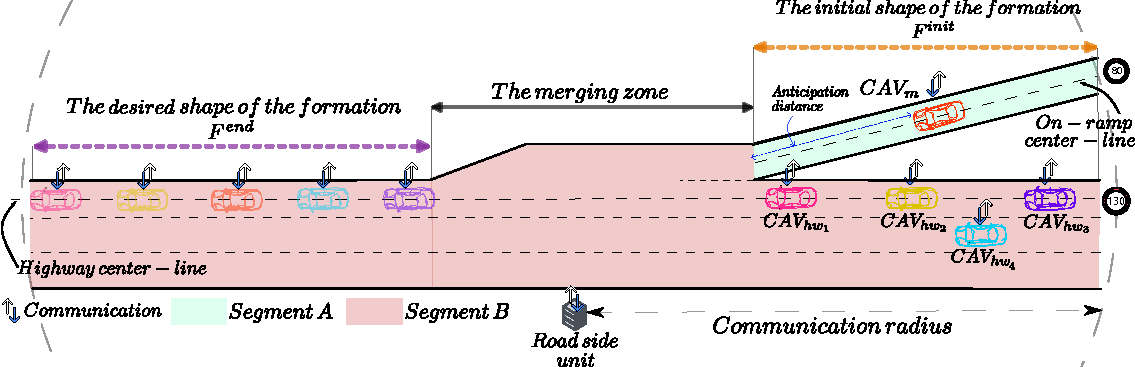
\includegraphics[width=12.5cm,height=18cm,keepaspectratio]{chapters/Chapitre_5/Figures/ScenarioScene.pdf}
        %\vspace{-2.3mm}
        \caption{Illustration of the on-ramp merging scenario based on the road segmentation strategy}
        \label{fig:Road_Segmentation}
        %\vspace{-5mm}
        \end{figure}

The proposed MVS control architecture relies on the existence of a global reference path that vehicles need to follow to perform their driving maneuver. Consequently, the aim of the optimization algorithm part of the CORM framework was to approximate the reference path when generating the virtual targets of each vehicle of the formation. As discussed in Section \ref{sec:CORM_conclusion}, the CORM encounters some difficulties to generate an estimate that aligns with the global reference path. In order to take into account the vehicles reference path and overcome the CORM limitation related to the latter, in this section a segmentation strategy that takes explicitly the reference path is proposed part of the E-CORM algorithm. 

Taking advantage from the E-CORM flexibility, it is proposed to segment the merging scenario w.r.t. the vehicle's motion on each segment. Figure \ref{fig:Road_Segmentation} gives an illustration of the proposed segmentation strategy. Segment $A$ represents the portion of the scenario where the vehicles need to track their reference path, thus only the longitudinal reconfiguration of the formation is required. The segment $B$ lies on both the longitudinal and the lateral formation reconfiguration. 



\tikzstyle{decision} = [diamond, draw, fill=white!,
    text width=3 em, text badly centered, node distance=1.8cm, inner sep=1pt]
\tikzstyle{block} = [rectangle, draw, fill=white!,
    text width=20 em, text centered, minimum height=4em]
    \tikzstyle{case} = [rectangle, draw, fill=white!,
    text width=8 em, text centered, minimum height=6em]
\tikzstyle{line} = [draw, very thick, color=black, -latex']
\tikzstyle{cloud} = [draw, ellipse, fill=white!, node distance=1.2cm,
    minimum height=2em]
\begin{figure}[!h]
\begin{center}
    \begin{tikzpicture}[scale=2, node distance = 1cm, auto]
    % Place nodes


    \node [cloud] (n1) {\footnotesize Begin}; 
    \node [block, below of= n1,minimum height=1em,  minimum width=18em ,node distance= 0.9cm] (n2){\footnotesize{ V$_i$} localization};
    \node[decision, below of= n2,minimum height=1em, minimum width=8em, node distance=1.5cm ] (n3) {\footnotesize V$_i$ in Segment A}; 
    \node[case, below left of= n3, minimum height=3em, minimum width=2cm,node distance= 1.8cm, xshift=-1cm](n4){\footnotesize $h_i$ $\leftarrow$ E-CORM \\ $l_i$ $\leftarrow$ center-line};
    \node[case, below right of= n3, minimum height=3em, minimum width=2cm,node distance= 1.8cm, xshift=1cm](n5){\footnotesize $h_i, \, l_i$ $\leftarrow$ E-CORM};
    
    \node[decision, below of= n3,minimum height=1em, minimum width=8em, node distance=3.0cm ] (n6) {\footnotesize End of reconfig.}; 
    \node[cloud, below of= n6,node distance= 1.5cm] (n7){\footnotesize End};  

    % Draw edges 
    \path[line] (n1)--(n2);%node[text width=23.5em,text height=1em]; 
    \path[line] (n2)--(n3); 
    \path[line] (n3.west) node |-(-1.14,-1.2) node [text width=-2em, text height=2.3em]{\footnotesize Yes} --(n4.north); 
    \path[line] (n3.ouest) node |-(1.14,-1.2) node [text width=3em, text height=2.3em]{\footnotesize No} --(n5.north); 
   \path[line] (n4.south) --(n6.north); 
   \path[line] (n5.south) --(n6.north); 
   \path[line] (n6.west)  node [text width=3em,text height=2.3em]{\footnotesize No} node  -|(-2.2---,-0.45)  -- (n2.west) ;
   \path[line] (n6) node [text width=3em,text height=6em]{\footnotesize Yes}  --(n7); 
    \begin{pgfonlayer}{background}
   \end{pgfonlayer}

\end{tikzpicture}
\end{center}
\vspace{-4mm}
\caption{Coordinates selection based on the traveled segment}
\vspace{-3mm}%Put here to reduce too much white space after your table 
   \label{fig: E-CORM flowshart}

\end{figure} 
Furthermore, the optimization procedure to compute the extended constrained inter-target distance matrix (cf. Section \ref{sec:ReconfigurationGains}) can be expensive in terms of the computation time. Thus, the segmentation of the road topology permits to reduce the computation time by optimizing only the necessary gains part of reconfiguration matrix $A$. In other terms, when the vehicle travels on the segment $A$, only the longitudinal reconfiguration is necessary. Consequently, only the gains related to the longitudinal behavior are optimized (cf. Figure \ref{fig: E-CORM flowshart}). The lateral coordinates $l_i$ are given according to the road center-line. On the other hand, when both of the longitudinal and lateral behaviors are necessary (i.e., the vehicle travels in segment $B$), both of the gains $a_{h_{i}}$ and $a_{l_{i}}$ are optimized. This selection mode is possible thanks to the capacity of the algorithm to guarantee the continuity of the dynamic targets $T_d$ ensured by the formalism using the state $S$ (cf. equation \ref{eq:BasicInitialEquation}).  

\subsection{Simulation results}\label{sec:Simulation_E-CORM}



To assess the effectiveness of the E-CORM algorithm in terms of ensuring the safety and the smoothness of the vehicles' dynamic during the on-ramp merging maneuver, a simulation scenario similar to the one in Section \ref{sec:CORM_simulation} is proposed. The video of the simulation can be found in \textcolor{blue}{https://youtu.be/-h97Qz7K3F4}. 


In the following simulation, it is aimed to perform a merging maneuver with a formation of three vehicles. The considered merging scenario is an on-ramp merging where $V_1$ (i.e., the reference vehicle $V_R$) is placed in the main line, so as $V_2$. The third vehicle $V_3$ (the merging vehicle) is initially placed in the secondary on-ramp merging road (cf. Figure \ref{fig:E-CORM: formation_shape}). The initial formation shape is triangular (cf. Figure \ref{fig:E-CORM: formation_shape} (a)), consequently at the end of the reconfiguration phase, the aim is to put the vehicles part of the formation in a linear shape to form a platoon (cf. Figure \ref{fig:E-CORM: formation_shape}(c)). The minimum inter-target distance $\underline{D}_T$ is computed using eq. \ref{eq:minimum_distance_model}.




 
        \begin{figure}[!h]
        \centering 
        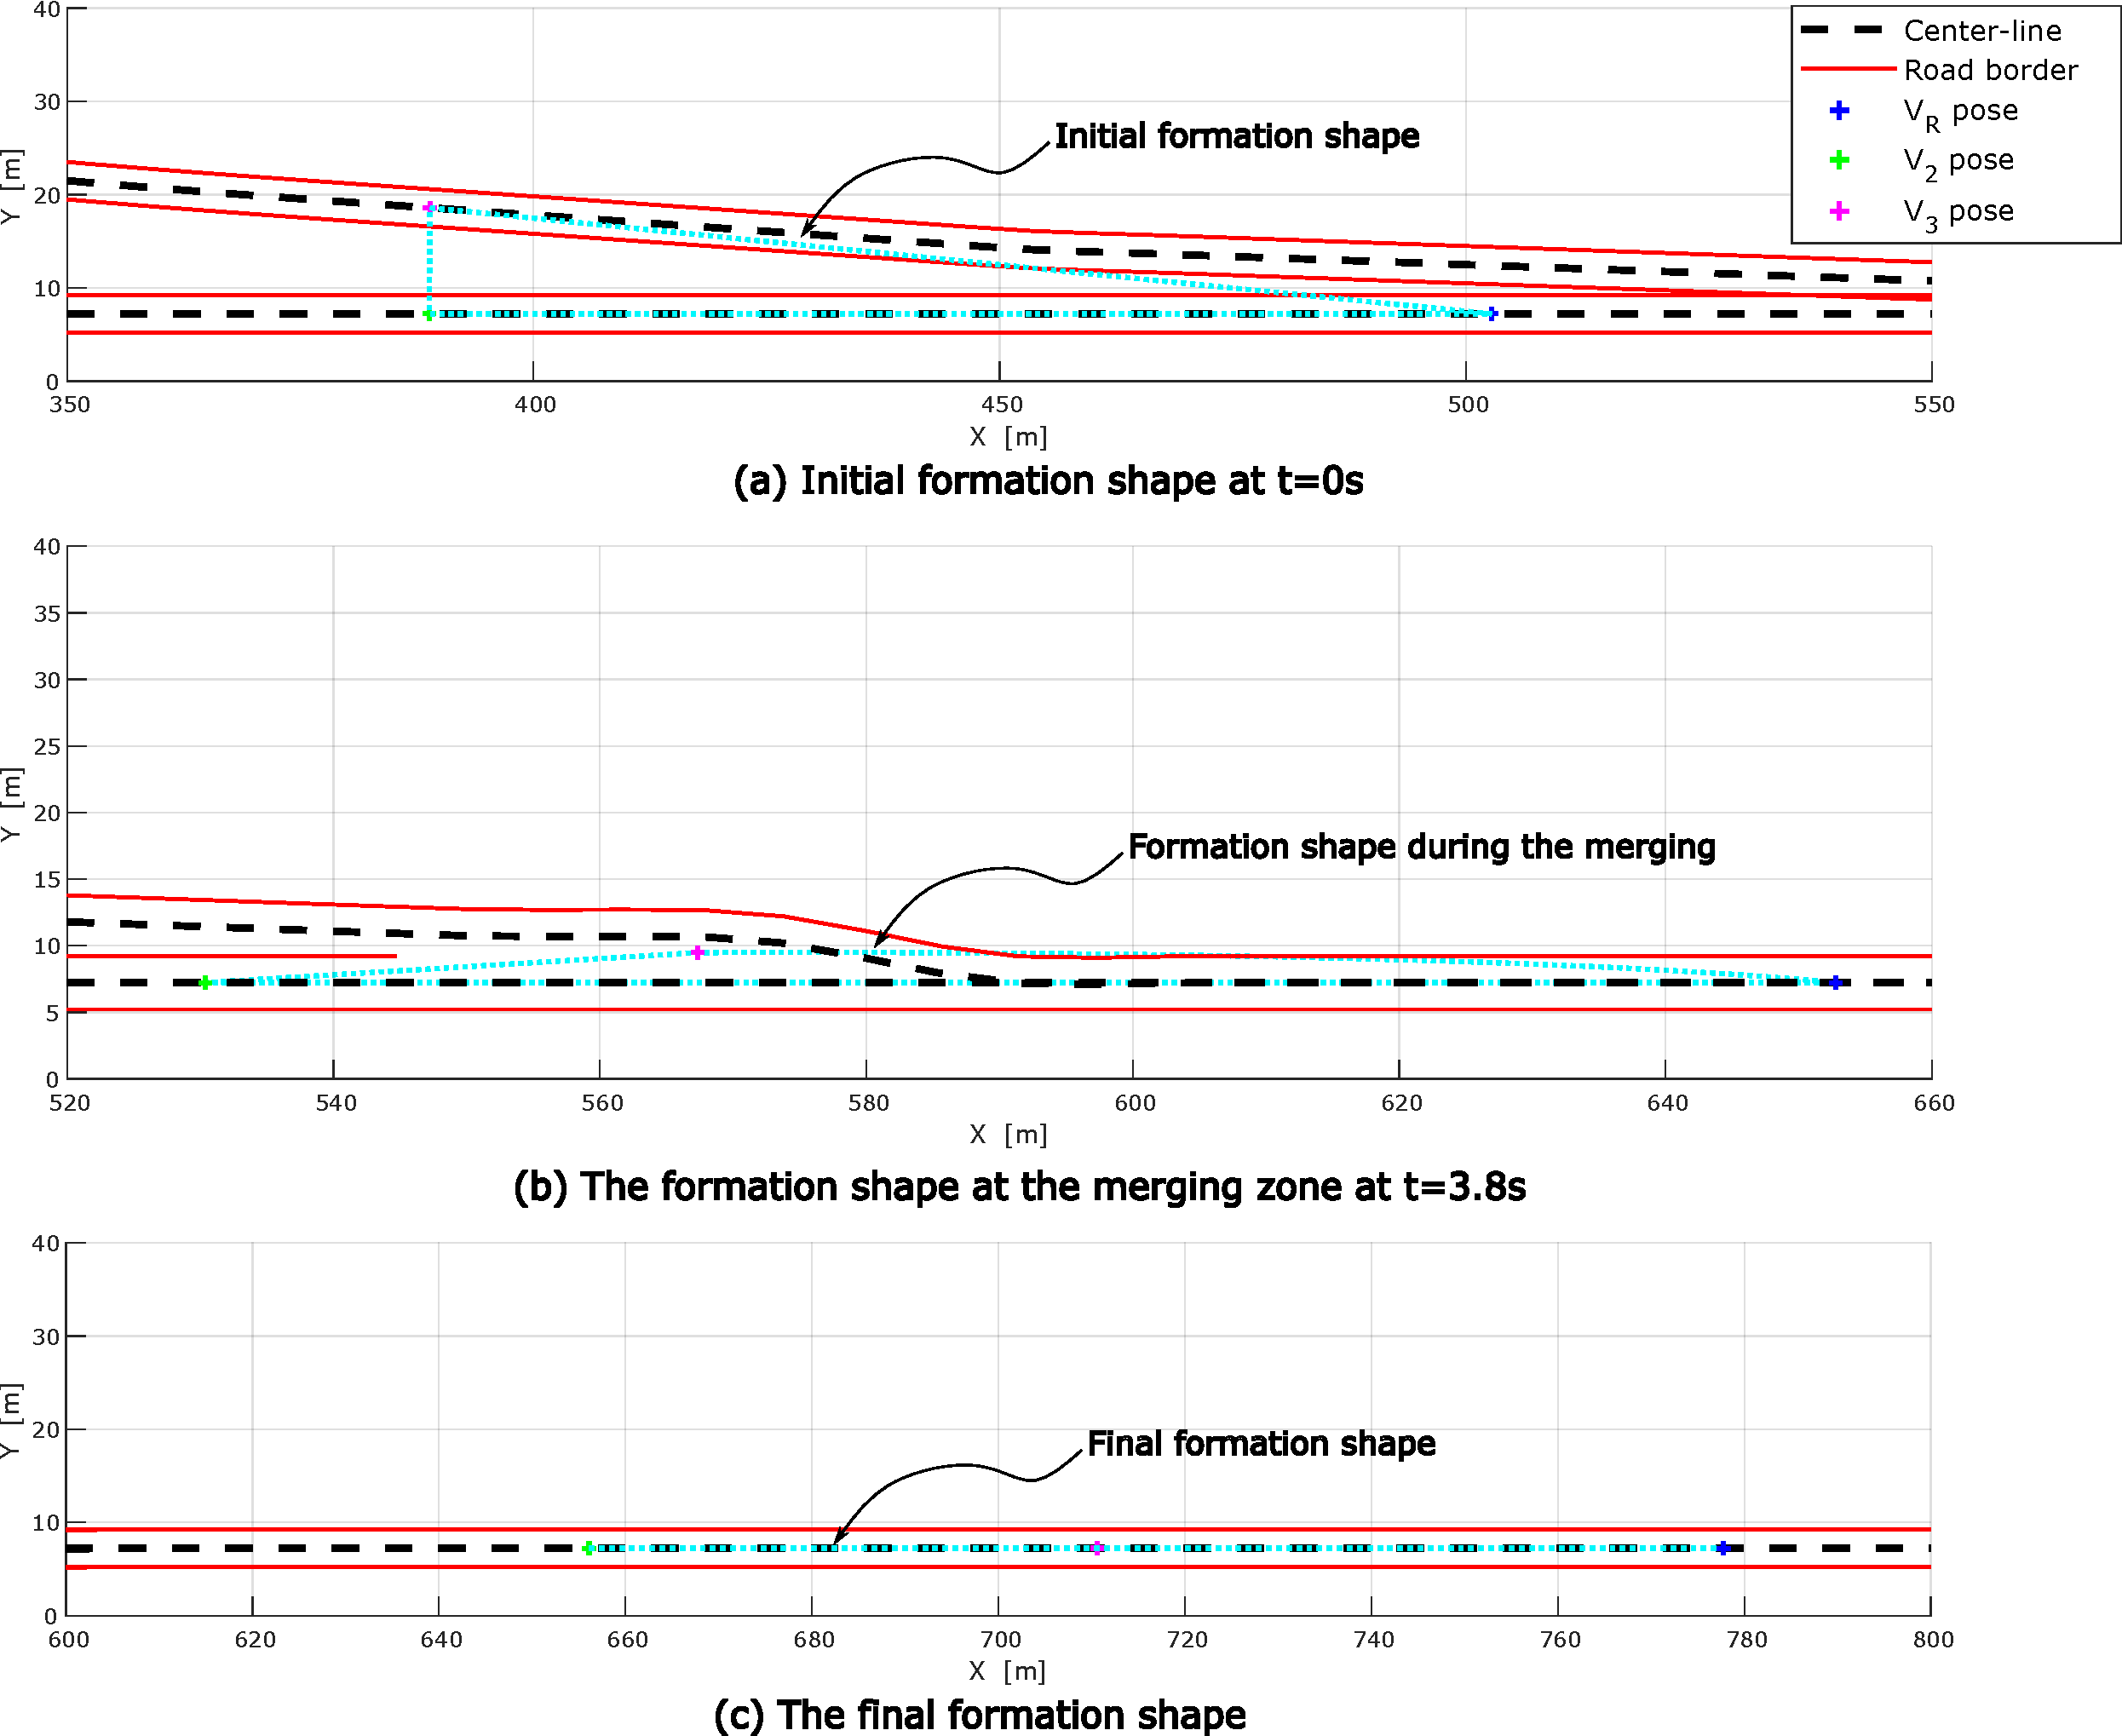
\includegraphics[width=12cm,height=18cm,keepaspectratio]{chapters/Chapitre_5/Figures/E-CORM/Formation_shape.pdf}
        %\vspace{-2.3mm}
        \caption{Evolution of the formation shape based on the E-CORM reconfiguration (\textcolor{blue}{Simulation video: https://youtu.be/-h97Qz7K3F4})}
        \label{fig:E-CORM: formation_shape}
        %\vspace{-5mm}
        \end{figure}


The reconfiguration of the triangular configuration into the desired linear one is visually represented in Figure \ref{fig:E-CORM: formation_shape}. In this process, the initial formation, defined by the original coordinates, undergoes a reconfiguration phase. During this phase, both vehicles $V_2$ and $V_3$ are positioned at approximately equi-longitudinal distance relative to $V_1$ ($V_R$). The intermediate formation illustrates the positions of all three vehicles within the conflict zone. As anticipated, the gap between $V_3$ and $V_1$ decreases, resulting in $V_3$ merging between $V_1$ and $V_2$ (cf. Figure \ref{fig:E-CORM: formation_shape} (b)). The final formation shape, as depicted in Figure \ref{fig:E-CORM: formation_shape} (c), shows the three vehicles within the formation now forming a platoon, aligning with the intended configuration. 



        \begin{figure}[!h]
        \centering 
        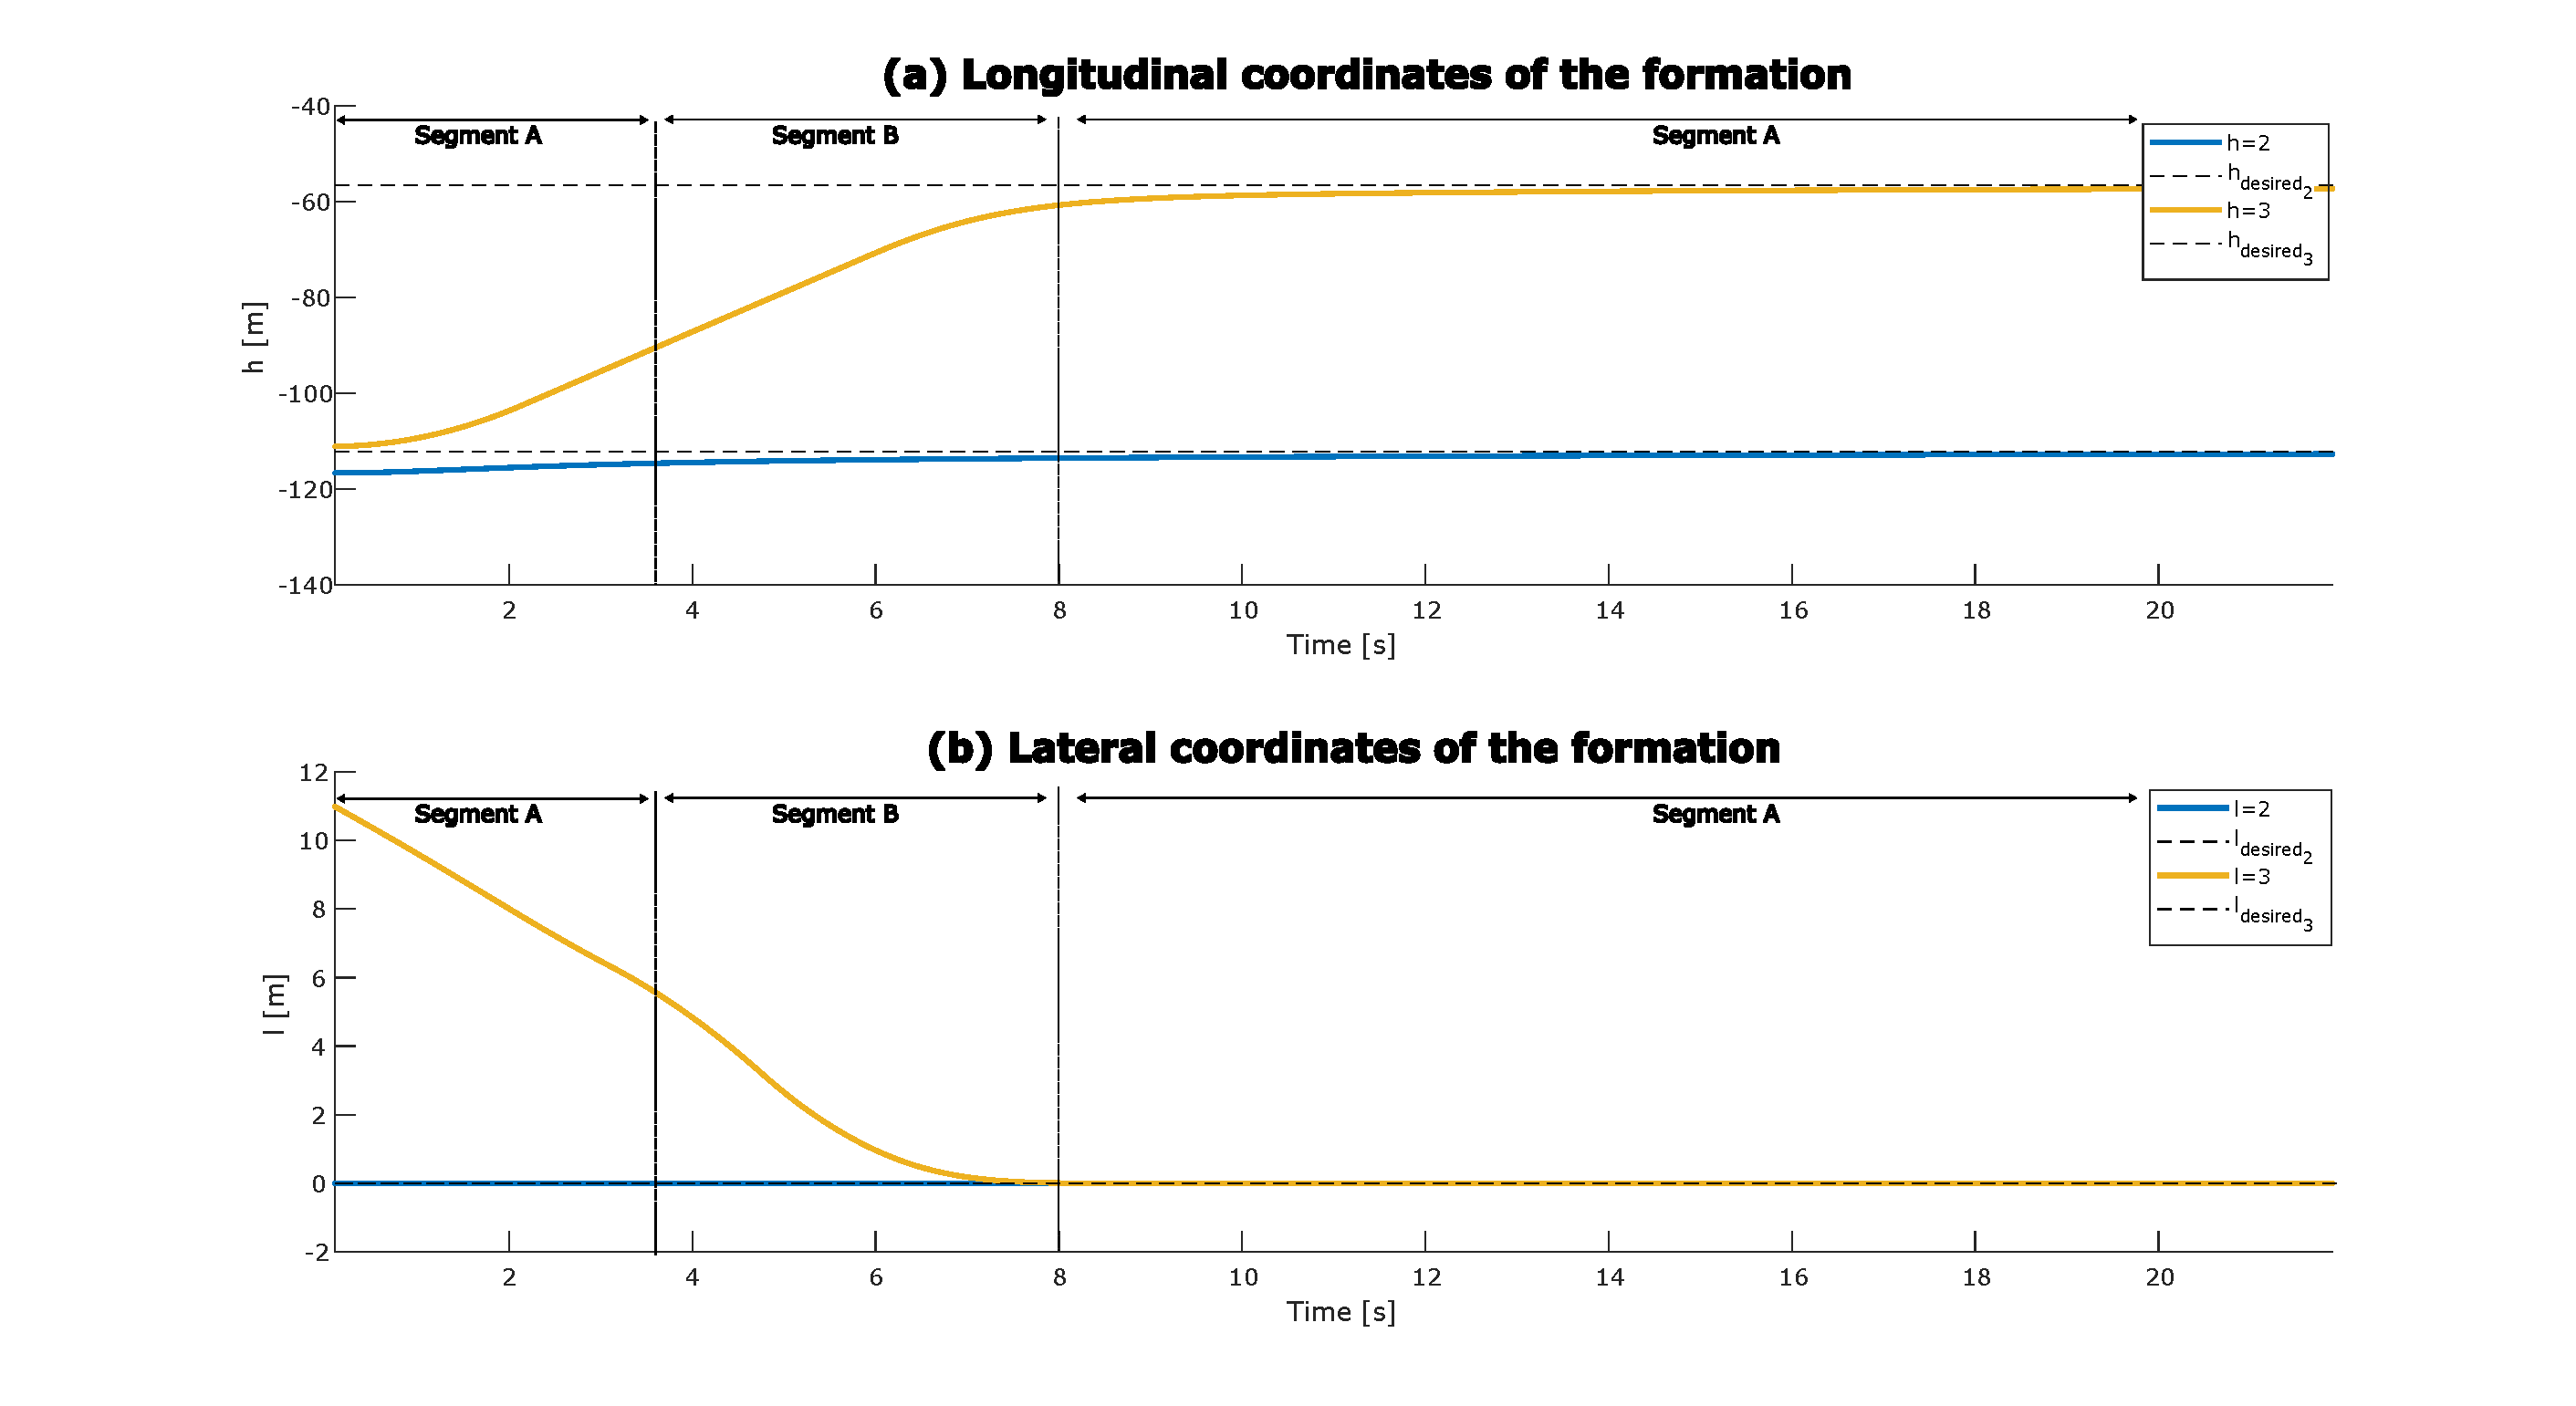
\includegraphics[width=14cm,height=18cm,keepaspectratio]{chapters/Chapitre_5/Figures/E-CORM/Formation_coordinates.pdf}
        %\vspace{-2.3mm}
        \caption{The formation's coordinates}
        \label{fig:E-CORM: formation_coordinates}
        %\vspace{-5mm}
        \end{figure}


To evaluate the E-CORM capability in terms of safety and convergence errors, it is proposed to study the evolution of the formation coordinates illustrated in Figure \ref{fig:E-CORM: formation_coordinates} and the in-between distances profiles illustrated in Figure \ref{fig:E-CORM: formation_distances}. In Segment $A$, only the E-CORM's longitudinal reconfiguration is activated, consequently, the lateral coordinates of $V_3$ are computed with the help of the reference path. In Segment $B$ both the longitudinal and the lateral reconfiguration are activated. As it can be seen in Figure \ref{fig:E-CORM: formation_coordinates}, the formation reconfiguration is almost complete by the end of Segment $B$. The Euclidean distances in-between the vehicles are greater than $\underline{D}_T$ (cf. Figure \ref{fig:E-CORM: formation_distances}), thus the merging is considered to be safe. When the three vehicles travel in highway, only the longitudinal reconfiguration is activated, thus, the formation continues its convergence toward the desired shape. 

        \begin{figure}[!h]
        \centering 
        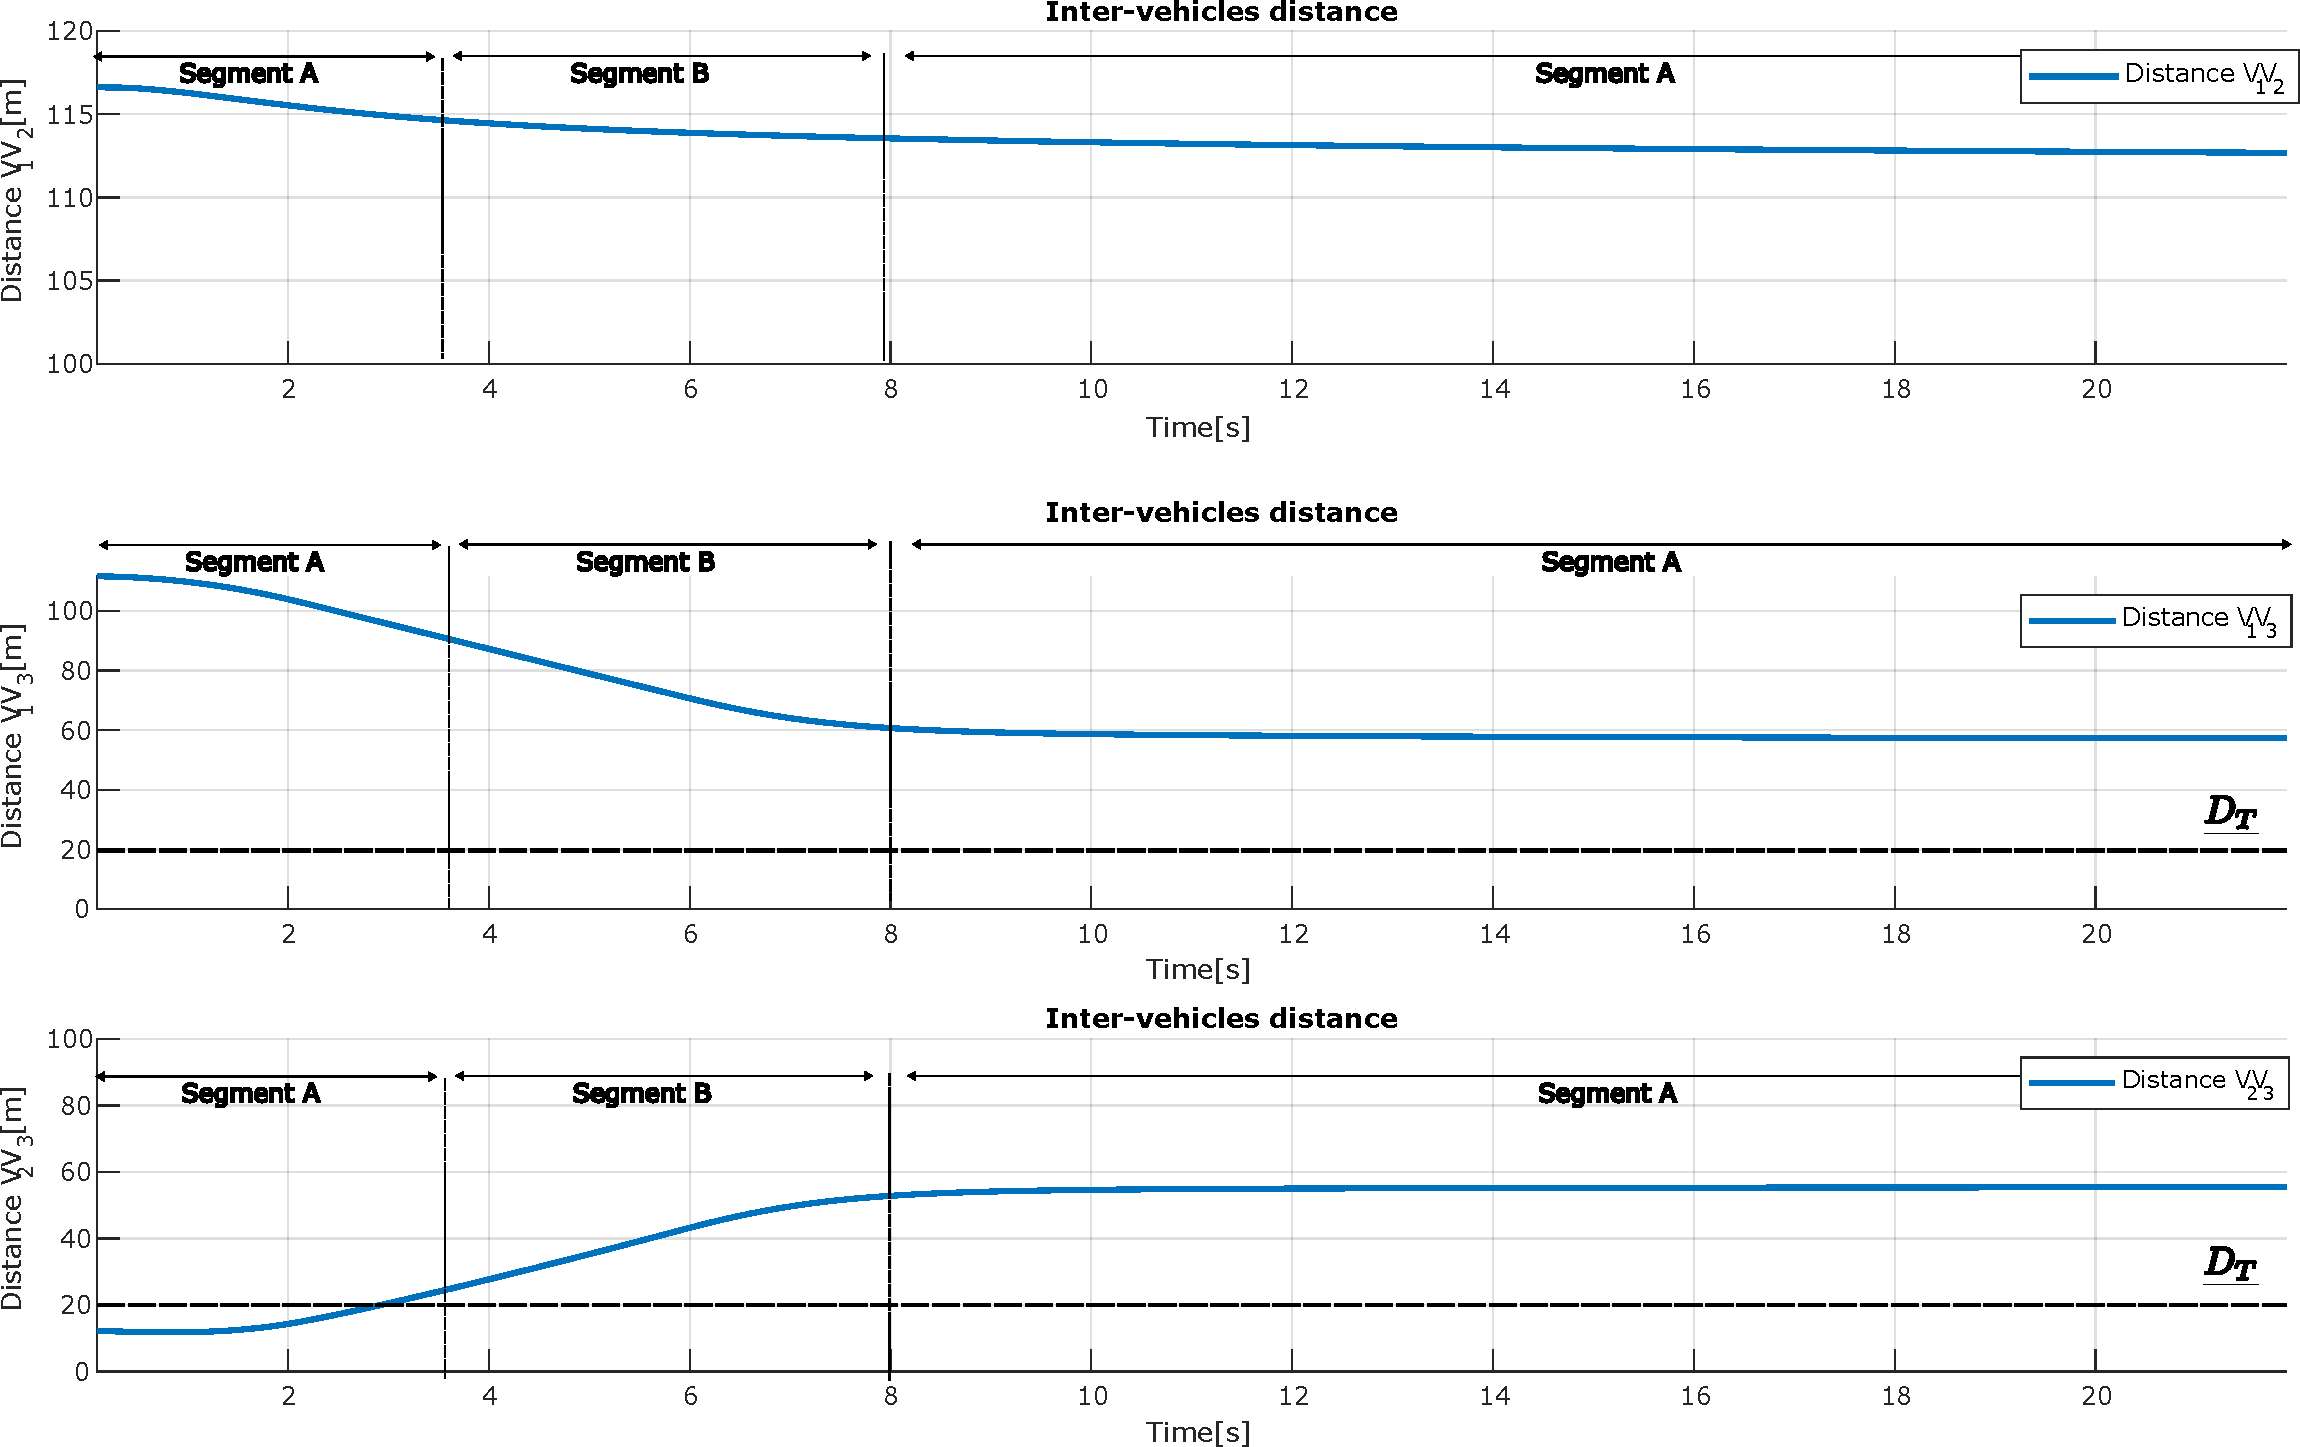
\includegraphics[width=12cm,height=18cm,keepaspectratio]{chapters/Chapitre_5/Figures/E-CORM/Distances.pdf}
        %\vspace{-2.3mm}
        \caption{The Euclidean in-between distances}
        \label{fig:E-CORM: formation_distances}
        %\vspace{-5mm}
        \end{figure}



In Figure \ref{fig:E-CORM: velocity}, the linear velocity is presented for each of the three vehicles part of the formation. As expected, the velocity of the vehicle $V_3$ increases in-order to reduce the gap between $V_1$ and $V_3$, before it decreases in order to respect the velocity requirement in the platoon. As for $V_2$, its velocity increases to converge toward its desired formation longitudinal coordinate, before it increases so that $V_2$ can travel part of the platoon with constant in-between distance w.r.t. $V_3$. 

        \begin{figure}[!h]
        \centering 
        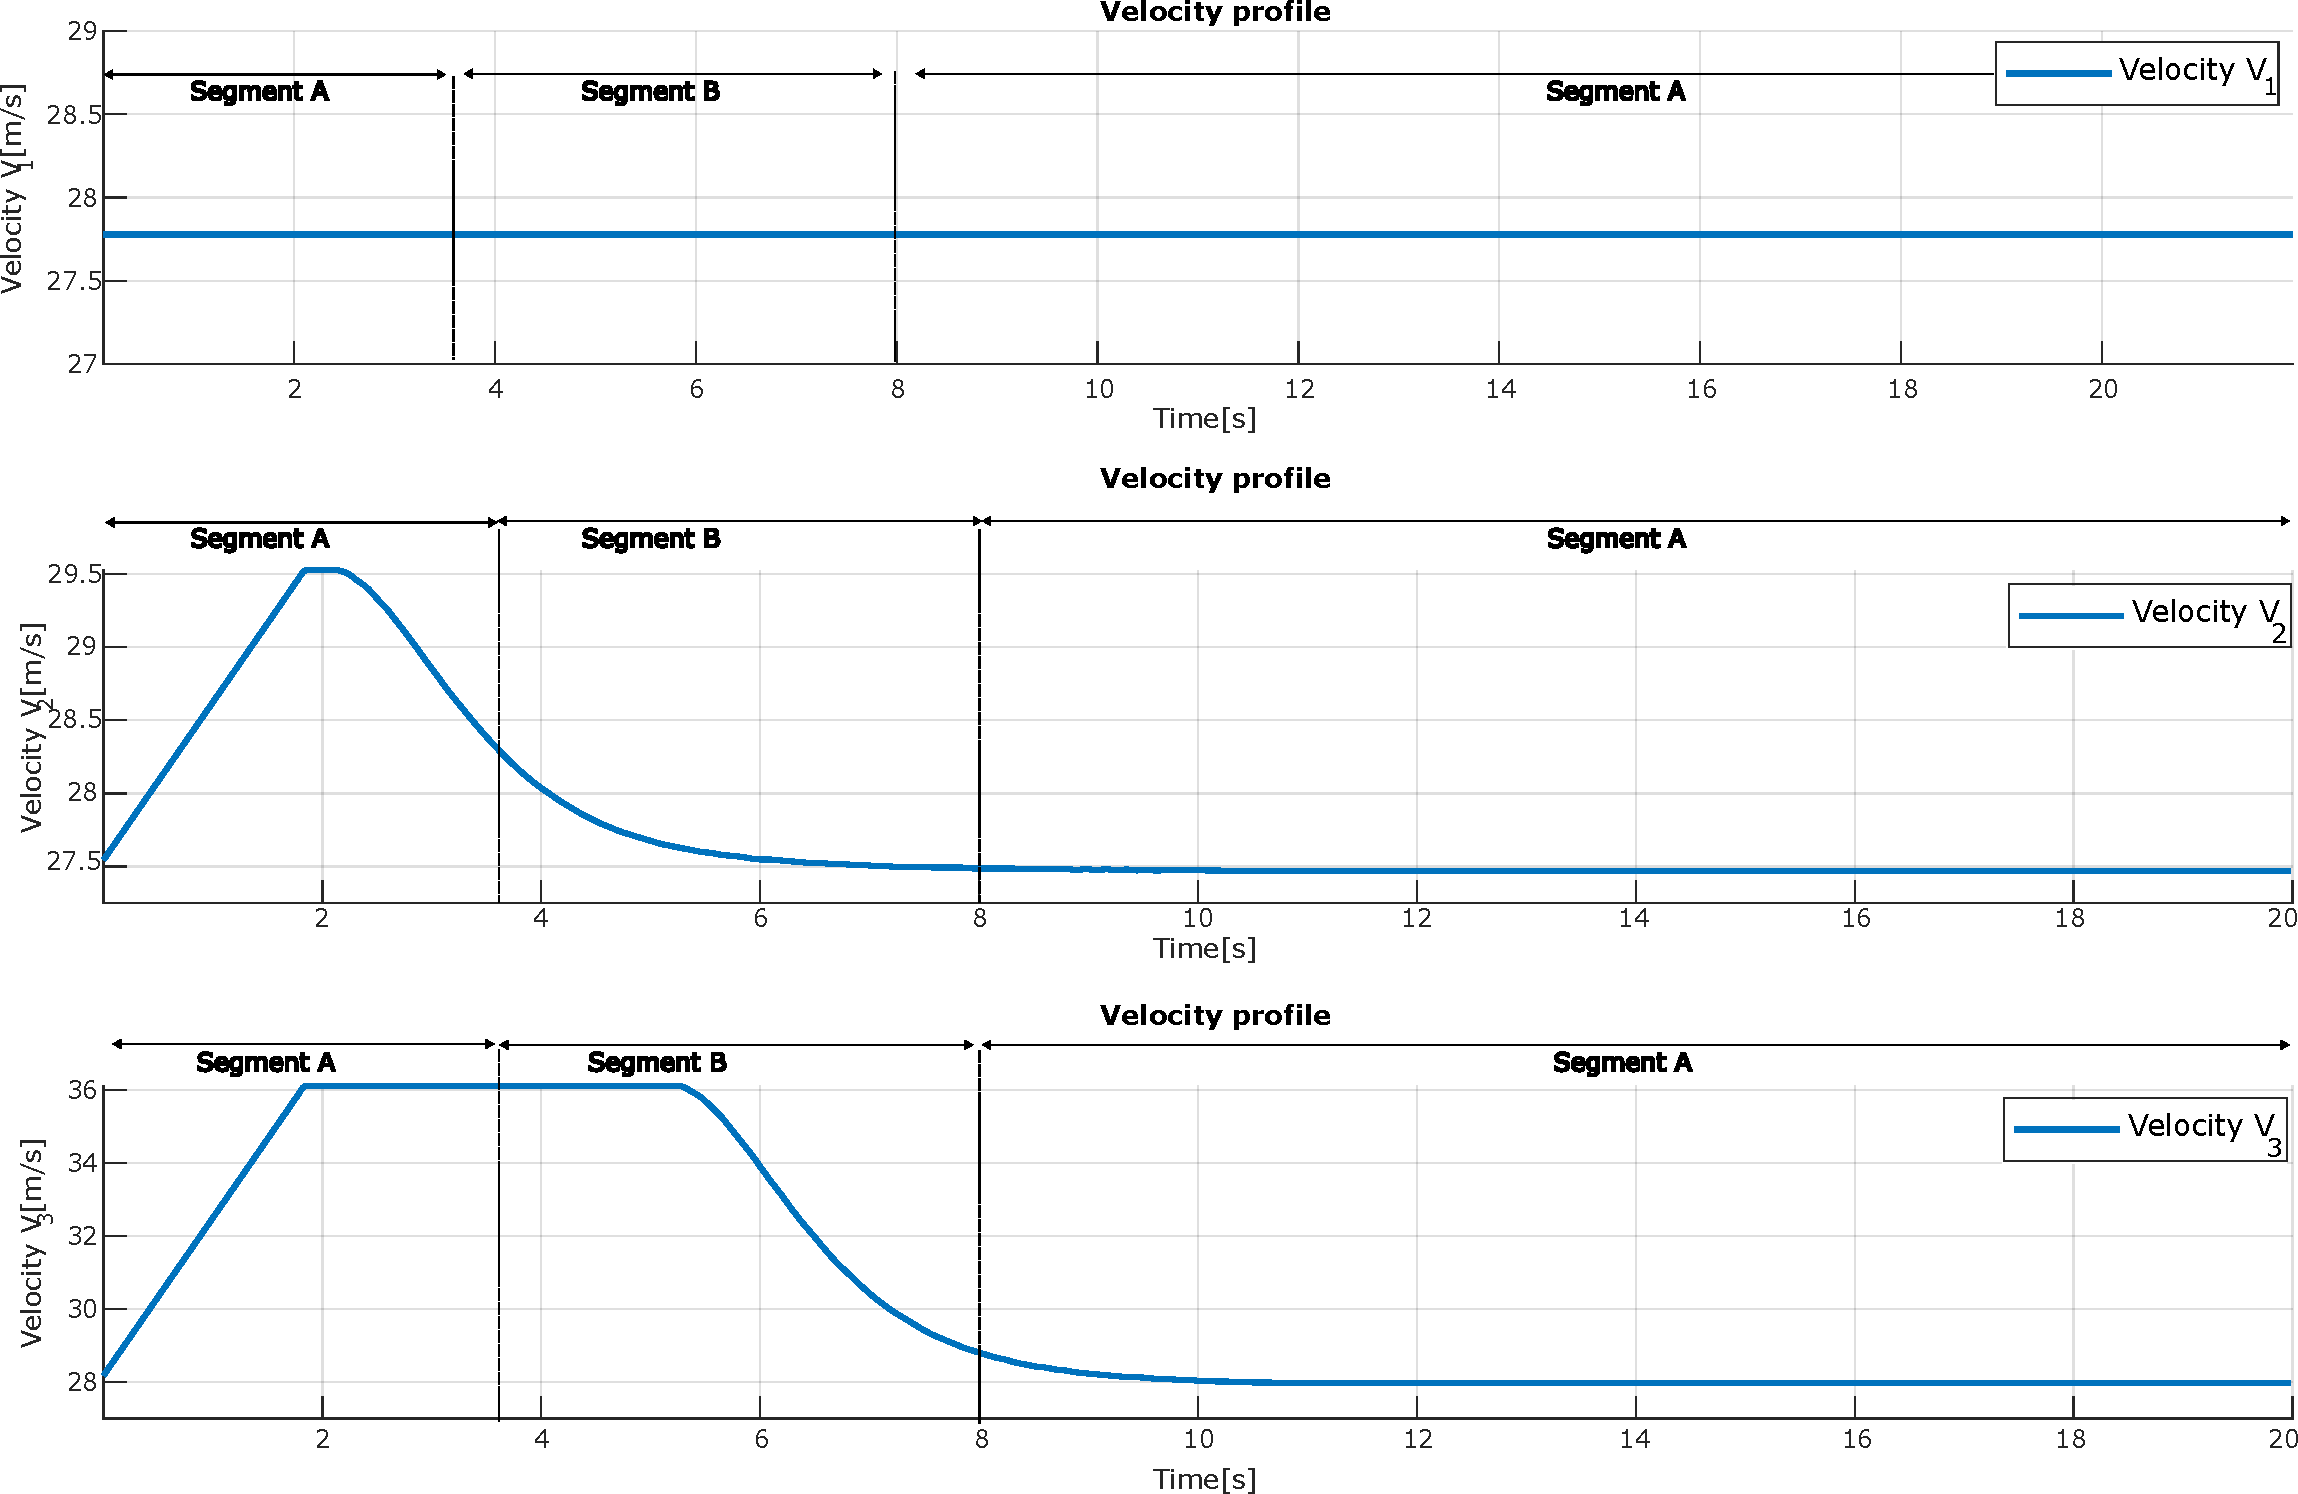
\includegraphics[width=12cm,height=18cm,keepaspectratio]{chapters/Chapitre_5/Figures/E-CORM/Velocity_profiles.pdf}
        %\vspace{-2.3mm}
        \caption{The vehicles' velocity profiles}
        \label{fig:E-CORM: velocity}
        %\vspace{-5mm}
        \end{figure}



\newpage
\subsection{Conclusion of the E-CORM algorithm} \label{sec:Conclusion_E-CORM}








This section delved extensively into the realm of cooperative formation reconfiguration, employing the proposed Extended Constrained Optimal Reconfiguration Matrix (E-CORM) framework. The primary goal behind introducing E-CORM was to address the CORM's lack of flexibility. 

E-CORM leverages an extended inter-target distance matrix, allowing for the reconfiguration of the formation during the merging, while introducing an enhanced level of motion flexibility. Unlike the restrictive nature of CORM, which obstruct vehicles from precisely following their global reference trajectory, and by the addition of the proposed extended inter-target distance matrix, the E-CORM overcomes this limitation by explicitly incorporating the global reference trajectory using the proposed road segmentation strategy. 

The road segmentation strategy plays a pivotal role in activating only the necessary vehicle behaviors concerning their position in the environment. Consequently, when vehicles are expected to remain on their reference path, only longitudinal reconfiguration is required. In contrast, when the merging vehicle enters the merging zone, both longitudinal and lateral reconfiguration are engaged to facilitate the merging process. Importantly, since E-CORM depends on an optimization process to compute the extended inter-target distance matrix gains, these computations are tailored to the activated behaviors, reducing the overall optimization time cost.



The evaluation of the E-CORM algorithm was carried out in a simulation environment. It showcased the algorithm's ability to adhere to safety criterion and its enhanced flexibility even in challenging scenarios involving high-speed merging. 


However, it's worth noting that E-CORM's reliance on a non-linear optimization algorithm to compute the extended inter-target distance matrix remains a notable limitation. This holds significance, especially given that one of the aims of this PhD work is to propose an online control architecture. The time-intensive nature of optimization algorithms does not align with the scope of this specific objective. In order to mitigate both of the CORM's and the E-CORM's limitations, in addition of achieving the objective of the decision/control architecture, in the following section the Formation Reconfiguration Approach based on an Online Control Strategies (FRA-OCS) is proposed. 


\section{Formation Reconfiguration Approach based on an Online Control Strategy (FRA-OCS)} \label{sec:No-opt}
As discussed in Section \ref{sec:CORM}, the CORM algorithm's lacks of motion flexibility constitute one of its main limitations. Consequently, in Section \ref{sec:E-CORM}, the E-CORM framework was proposed to overcome the CORM limitation. Through the study of the E-CORM performance, it was pointed out that its reliance on an optimization process constitutes a limitation w.r.t. the objective of this work, which is to propose an online control architecture. 

To overcome both the CORM's and the E-CORM's limitations, in this section an optimization-free formation reconfiguration algorithm named Formation Reconfiguration Approach based on an Online Control Strategies (FRA-OCS) is presented. 


Before the presentation of the details of the proposed FRA-OCS for formation reconfiguration, and for the clarity of this PhD manuscript and the understanding of the reader, it is important to note that the formation definition and configuration formalism used part of the FRA-OCS is the same as the one used for the CORM (cf. Section \ref{sec:formation_modeling_section}). 


Section \ref{sec:FRA-OCS} delves into the proposed FRA-OCS formalism, additionally Section \ref{sec:Computation_section} provides the details related to dynamic generator part of the proposed FRA-OCS. The FRA-OCS performance is evaluated through a simulation scenario in Section \ref{sec:Simulation_FRA-OCS}. Lastly, it is proposed to draw conclusion about the FRA-OCS in Section \ref{sec:Conclusion_FRA-OCS}.  


\subsection{FRA-OCS formalism} \label{sec:FRA-OCS}
Prior to delving into the specifics of the proposed Formation Reconfiguration Approach based on an Online Control Strategy (FRA-OCS), for the clarity and the understanding of the reader, it is important to note that the fundamentals related to the virtual structure formalization used to represent the formation of vehicles can be found in Section \ref{sec:formation_modeling_section}. 


To address the limited flexibility of both the CORM (cf. Section \ref{sec:CORM}) and the E-CORM (cf. Section \ref{sec:E-CORM}) algorithms, the FRA-OCS introduces an intermediate state, $S$, as an essential component for characterizing the evolution of the reconfiguration process from the initial shape of the formation to its desired shape. By employing this intermediate state vector, the FRA-OCS enables a smooth and controlled transition of the formation towards its desired shape. Eq. \ref{eq:BasicInitialEquation-FRA} provides the explicit expression of the intermediate state vector $S$.  

\begin{equation} \label{eq:BasicInitialEquation-FRA}
    S = \dot{e} + \lambda e \\
\end{equation}

The FRA-OCS utilizes in addition to the convergence error vector $e$ (cf. Section \ref{sec:formation_modeling_section}), the convergence rate $\dot{e}$. By introducing the gain  $\lambda \;  \in \mathbb{R}^+ $, the FRA-OCS offers greater flexibility in achieving the desired formation reconfiguration. 

The use of an optimization approach allows the computation of reconfiguration gains within the CORM algorithm (cf. Section \ref{sec:CORM}). By combining the longitudinal and lateral motions, the computation time required for optimization is reduced. However, one drawback of this motion coupling is its limited flexibility. The state $S$ used in the E-CORM (cf. eq. \ref{eq:BasicInitialEquation}) is composed of a proportional, a derivative, and an integrative terms. However, in the final form in the FRA-OCS, the state $S$ was chosen to use only the proportional and the derivative terms. This choice is mainly motivated by the need of a simplified mathematical representation to facilitate the on-line identification of the different gains involved. As a result, in addition to the state vector $S$ used by the FRA-OCS, the proposed approach suggests to use the road segmentation strategies proposed in Section \ref{sec:RoadSegmentationStrategie}, decoupling the longitudinal convergence from the lateral convergence. Figure \ref{fig:Road_Segmentation} illustrates the segmentation approach based on the road geometry used to define the available vehicle motion according to its position. 

The convergence of $S$ follows a first order convergence model detailed in eq. \ref{eq:BasicInitialEquation2-FRA}. 

\begin{equation} \label{eq:BasicInitialEquation2-FRA}
    \dot{S} = A \times S = A \dot{e} +  A \lambda e  \\
\end{equation}
where $A^{2N\times 2N}$ is a negative-definite convergence matrix.


Using eq. \ref{eq: errorbetweenfinitandfendforvi} in eq. \ref{eq:BasicInitialEquation2-FRA} permits to write the extended system of equations representing the formation reconfiguration studied system. 

\begin{eqnarray} \label{eq:SystemOfBasicEquation_simplified}
  \dot{S}_{h_{1}} &=& a_{h_{1}}\dot{e}_{h_{1}} + a_{h_{1}}\lambda_{h_{1}}e_{h_{1}}\\ \nonumber
  \dot{S}_{l_{1}} &=& a_{l_{1}}\dot{e}_{l_{1}} + a_{l_{1}}\lambda_{l_{1}}e_{l_{1}}\\ \nonumber
        &\vdots& \\ \nonumber
  \dot{S}_{h_{N}} &=& a_{h_{N}}\dot{e}_{h_{N}} + a_{h_{N}}\lambda_{h_{N}}e_{h_{N}}\\ \nonumber
  \dot{S}_{l_{N}} &=& a_{l_{N}}\dot{e}_{l_{N}} + a_{l_{N}}\lambda_{l_{N}}e_{l_{N}}\\ \nonumber
\end{eqnarray}
                \vspace{-8.5mm}

\noindent where $h_i$ and $l_i$, representing the longitudinal and the lateral coordinates of the formation, converge toward the target with different convergence rates $a_{h_i}$ and $a_{l_i}$. 

The system in eq. \ref{eq: reconfiguration matrix} presents the matrix form of the studied system.


%% the reconfiguration matrix 
\begin{equation}\label{eq: reconfiguration matrix}
\begin{bmatrix} 
\dot{S}_{h_{1}} \\
\dot{S}_{l_{1}} \\
% \dot{S}_{h_{2}} \\
% \dot{S}_{l_{2}} \\
\vdots \\
\dot{S}_{h_{N}} \\
\dot{S}_{l_{N}} \\
\end{bmatrix}= 
 \Omega_{1}
  \begin{bmatrix} 
\dot{e}_{h_{1}} \\
\dot{e}_{l_{1}} \\
% \dot{e}_{h_{2}} \\
% \dot{e}_{l_{2}} \\
\vdots \\
\dot{e}_{h_{N}} \\
\dot{e}_{l_{N}} \\
\end{bmatrix}+
\Omega_{2}
  \begin{bmatrix} 
 {e}_{h_{1}} \\
{e}_{l_{1}} \\
% {e}_{h_{2}} \\
% {e}_{l_{2}} \\
\vdots \\
{e}_{h_{N}} \\
{e}_{l_{N}} \\
\end{bmatrix}
\end{equation}


%% the details of the reconfiguration matrix 
\noindent with $\Omega_{1}=diag[a_{h_{1}},a_{l_{1}},\cdots,a_{h_{N}},a_{l_{N}}]$ and   \\ $\Omega_{2}=diag[a_{h_{1}}\lambda_{h_{1}},a_{l_{1}}\lambda_{l_{1}},\cdots,a_{h_{N}}\lambda_{h_{N}},a_{l_{N}}\lambda_{l_{N}}]$.

\subsubsection*{Stability analysis w.r.t. the convergence gains}
The stability of the system given in eq. \ref{eq: reconfiguration matrix} is proved in two steps; 1) the stability analysis of the state $S$ in the system in eq. \ref{eq:BasicInitialEquation2-FRA} using a Lyapunov analysis %\cite{Lyapunov} 
and; 2) the stability of the convergence error $e$ using the system given in eq. \ref{eq:SystemOfBasicEquation_simplified}. The details of the stability demonstration can be found in Section \ref{sec:stability_analysis}

% First, the Lyapunov candidate function is defined: 
% \begin{equation} \label{eq: lyapunov function}
%     V= \frac{1}{2}S^{T}S
% \end{equation}

% $V$ is a positive-definite function. To guarantee the stability of the system, $\dot{V}$ must be negative-definite. By taking the derivative of eq. (\ref{eq: lyapunov function}) and using eq. \ref{eq:BasicInitialEquation2-FRA}. $\dot{V}$ can be written: 
% \begin{equation}\label{eq: derivative lyaponuv}
%     \dot{V}= \dot{S}^{T}S = S^{T}A^{T}S
% \end{equation}

% Since $A^T$ is a diagonal negative-definite matrix, then $\dot{V} < 0$ and the state $S$ converges asymptotically to zero.

% The second step of the stability analysis is to prove the convergence of the formation error system given in eq. \ref{eq:BasicInitialEquation-FRA}. The stability analysis of eq. \ref{eq: derivative lyaponuv} permits to write around the equilibrium point of the state $S$: 
% \begin{equation}\label{eq: convegrence equation}
% \begin{cases}
% \dot{S}=0 \\ 
% S=0
% \end{cases}
% \end{equation}

  

% Considering eq. \ref{eq: convegrence equation}, the convergence of the error $e$ in eq. \ref{eq:BasicInitialEquation-FRA} is studied according to the stability of a first order system, where the convergence of the system is ensured if and only if $\lambda$ is positive. 

\subsection{Online reconfiguration gains identification and velocity profile generation} \label{sec:Computation_section}

 One limitation of the formation reconfiguration based on both the CORM and the E-CORM is their dependency on an optimization process. In fact, the calculation of optimization-based reconfiguration gains may not be adequate for online calculation, especially, when $N$ vehicles are part of the formation and $2\times N$ gains (decoupled longitudinal and lateral motions are considered) need to be computed. Considering an on-road environment, in one hand, the approach ability to compute and recompute when necessary the reconfiguration gains is mandatory to guarantee the respect of the safety criterion, explicitly in a highly dynamic environment. In the other hand, due to the dynamic nature of the considered scenario, the approach needs to guarantee the continuity of the vehicles' dynamics during the switch from one configuration to another.  
 
 Consequently, the FRA-OCS proposed in this work is designed to overcome the CORM limitation in terms of its real-time computation, with an optimization free procedure to compute the reconfiguration gains. As for the FRA-OCS ability to recompute the convergence gains when necessary, under the FRA-OCS formalism the continuity during the switch from one configuration to another is formally ensured. This section presents the procedure employed to write the system of equation that needs to be solved to reconfigure the formation from the initial shape to the final, while taking into account the initial and the desired dynamics of the vehicles part of the formation. 

Using eq. \ref{eq:BasicInitialEquation-FRA} in eq. \ref{eq:BasicInitialEquation2-FRA}, the convergence model of the formation reconfiguration error is a system of second order linear differential equations, given in eq. \ref{eq:SystemOfBasicEquation}. 


\begin{eqnarray} \label{eq:SystemOfBasicEquation}
\ddot{e}_{h_{1}} + (\lambda_{h_{1}}-a_{h_{1}}) \dot{e}_{h_{1}} - a_{h_{1}}\lambda_{h_{1}}e_{h_{1}}&=& 0\\ \nonumber
\ddot{e}_{l_{1}} + (\lambda_{l_{1}}-a_{l_{1}}) \dot{e}_{l_{1}} - a_{l_{1}}\lambda_{l_{1}}e_{l_{1}}&=& 0\\ \nonumber
        &\vdots& \\ \nonumber
  \ddot{e}_{h_{N}} + (\lambda_{h_{N}}-a_{h_{N}}) \dot{e}_{h_{N}} - a_{h_{N}}\lambda_{h_{N}}e_{h_{N}}&=& 0\\ \nonumber
  \ddot{e}_{l_{N}} + (\lambda_{l_{N}}-a_{l_{N}}) \dot{e}_{l_{N}} - a_{l_{N}}\lambda_{l_{N}}e_{l_{N}}&=& 0\\ \nonumber
\end{eqnarray}


The general solution $x(t)$ (representing the general form of $e_i$ and its derivatives) of the system in eq. \ref{eq:SystemOfBasicEquation} can be written as: 

\begin{equation}\label{eq:solutionofDFE}
x(t) = \alpha_1 e^{\beta_1t} + \alpha_2 e^{\beta_2 t}   
\end{equation}

\noindent where $\beta_1$ and $\beta_2$ are the roots of the second order linear differential equation related to $x(t)$, and $\alpha_1$ and $\alpha_2$ are the gains related to the initial and final conditions of the solution. 

  
  
The system in eq. \ref{eq:ConvergenceModel} is the proposed velocity profile generator model used to compute the needed vehicle's velocity to reconfigure the formation from the initial shape toward its desired one. The generator model is inspired from eq. \ref{eq:solutionofDFE}. The latter is used to control the convergence rate of the coordinates $h$ and $l$ with the help of five degrees of freedom (DOFs) $K_1$, $K_2$, $a$, $\lambda$ and $c$.




\begin{equation} \label{eq:ConvergenceModel}
    \mathcal{V}(t) = K_1 e^{a t} + K_2 e^{-\lambda t} + c \\
\end{equation}

 \noindent with $a$ and $\lambda$ being the roots of the differential equation in eq. \ref{eq:SystemOfBasicEquation}. $K_1$, $K_2$ and $c$ are the gains used to take into account the initial and final conditions imposed to the velocity generator. The procedure used to solve the system in eq. \ref{eq:SystemOfBasicEquation} by the identification of the five DOFs of the velocity profile generator is described above: 

\begin{enumerate}
 
    \item In order to generate a velocity profile that takes into account explicitly the anticipation distance available to perform the merging, it is proposed to introduce the time $t_{max}$. The latter permits to set the moment where ${\mathcal{V}}$ reaches its maximum, hence the acceleration $\dot{\mathcal{V}}$ is zero as expressed in eq. \ref{eq:ConvergenceModelAcceleration}. Consequently, $t_{max}$ permits to dynamically adapt the acceleration dynamic of the vehicles w.r.t. the length of the anticipation zone. 
 

 
%  \textcolor{red}{when the anticipation distance to reach the merging zone is small, the values of $t_{max}$ needs to guarantee the respect of the safety criterion the formation. In contrary, for a scenario where the formation can benefit from a large anticipation distance, $t_{max}$  is selected make the best use the latter in addition to ensures the respect of the safety criterion.  }

\begin{equation} \label{eq:ConvergenceModelAcceleration}
    \dot{\mathcal{V}}(t_{max}) = aK_1 e^{a t_{max} } -\lambda  K_2 e^{-\lambda t_{max} }  = 0
\end{equation}


\item  The velocity profile generator in eq. (\ref{eq:ConvergenceModel}) needs to take into account the initial velocity of the vehicles and the desired one at the end of the reconfiguration. 

Thus $c=\mathcal{V}^{init} - K_1 -K_2 $ is computed to impose the initial velocity.
%, eq. (\ref{eq:VelocityConstraints1}) is used. 

%\begin{eqnarray} \label{eq:VelocityConstraints1}
%    c &=& \mathcal{V}^{init} - K_1 -K_2 
%\end{eqnarray}

In order to impose the final velocity $\mathcal{V}(t=t_f)=\mathcal{V}^{end}$, with $\mathcal{V}^{end}$ is the velocity of the reference vehicle, the eq. \ref{eq:VelocityConstraints2} is introduced.

\begin{equation} \label{eq:VelocityConstraints2}
     K_1 e^{a t_{f} } + K_2 e^{-\lambda t_{f} }  - K_1 -K_2  +\mathcal{V}^{init} -\mathcal{V}^{end}= 0\\
\end{equation}

\item Based on eq. \ref{eq:ConvergenceModel}, the expression of the position $P(t)$ of the vehicle can be written as in eq. \ref{eq:PositionConstraint}. 

\begin{equation} \label{eq:PositionConstraint}
    P(t)= \frac{K_1}{a} e^{a t } - \frac{K_2}{\lambda} e^{-\lambda t }   + (\mathcal{V}^{init}- K_1 -K_2 )t +d \\
\end{equation}

The term $d=P_0 - \frac{K_1}{a} + \frac{K_2}{\lambda}$ is used to impose the initial position $P_0$ of the vehicle at $t=0$. 

\item Let us define $M(t)$ as the coordinate of the vehicle in the formation and $M^{end}$ is its desired final coordinate. $M$ can be either a longitudinal coordinate or a lateral one. In order to link the proposed convergence model to the coordinates used in the virtual structure formalism, eq. \ref{eq:LinkConstraint1} is proposed. 


\begin{equation} \label{eq:LinkConstraint1}
    M(t)= P_{ref} - P(t) \\
\end{equation}

\noindent with $P_{ref}=\mathcal{V}_{ref}*t + P_{ref_0}$ is the pose of the reference vehicle and $\mathcal{V}_{ref}$ is the reference vehicle's velocity, said to be constant according to the Frenet based coordinates system used by the virtual structure approach. 

To guarantee that the desired final coordinate is reached by the vehicle at $t=t_f$ (i.e., $M(t_f)=M_f$), eq. \ref{eq:LinkConstraint} is used. 

  
 \begin{align}\label{eq:LinkConstraint}
        ( \mathcal{V}_{ref} t_f + P_{ref_0})  - \big[\frac{K_1}{a}e^{at_f} - \frac{K_2}{a}e^{-\lambda t_f} + \\ (\mathcal{V}_{min} - K_1 - K_2)t_f  + P_0  - \frac{K_1}{a} + \frac{K_2}{\lambda} \big] -M_f =0
 \end{align}


To solve equations (\ref{eq:ConvergenceModelAcceleration}), (\ref{eq:VelocityConstraints2}) and (\ref{eq:LinkConstraint}), a numerical solver is employed. Following this, a prediction step is initiated using the generated velocity profiles and the initial conditions of the formation. Subsequently, the numerical solution is evaluated based on the satisfaction of the safety criterion and the dynamic feasibility (e.g., respect of the acceleration limits, the maximum authorized velocity, etc.).



As an example, when the formation reconfiguration takes into account longitudinal motion, a longitudinal velocity profile is generated based on the initial and final conditions and dynamics (cf. Figure \ref{fig:Road_Segmentation}, Segment A in green). Similarly, when both of the longitudinal and the lateral motions are the responsibility of the formation reconfiguration strategy, both velocity profiles are generated for the the longitudinal and lateral motions (cf. Figure \ref{fig:Road_Segmentation}, Segment B in red). 

\end{enumerate}




\subsection{Simulation results}\label{sec:Simulation_FRA-OCS}
To access the effectiveness of the proposed FRA-OCS in ensuring the safety criterion and the dynamics smoothness of the formation reconfiguration during the on-ramp merging on highway, the evaluation focuses on analyzing the simulation results of merging scenario similar to the one proposed in Section \ref{sec:CORM} and Section \ref{sec:E-CORM}. The simulation video can be found in \textcolor{blue}{https://youtu.be/3gDSq5L3m-c}. 





The following simulation aims to perform the merging scenario of a formation composed of four vehicles (three highway vehicles and one merging vehicle) illustrated in the initial shape of the formation in Figure \ref{fig:FRA-OCS:formation_shape}. 

        \begin{figure}[!h]
        \centering 
        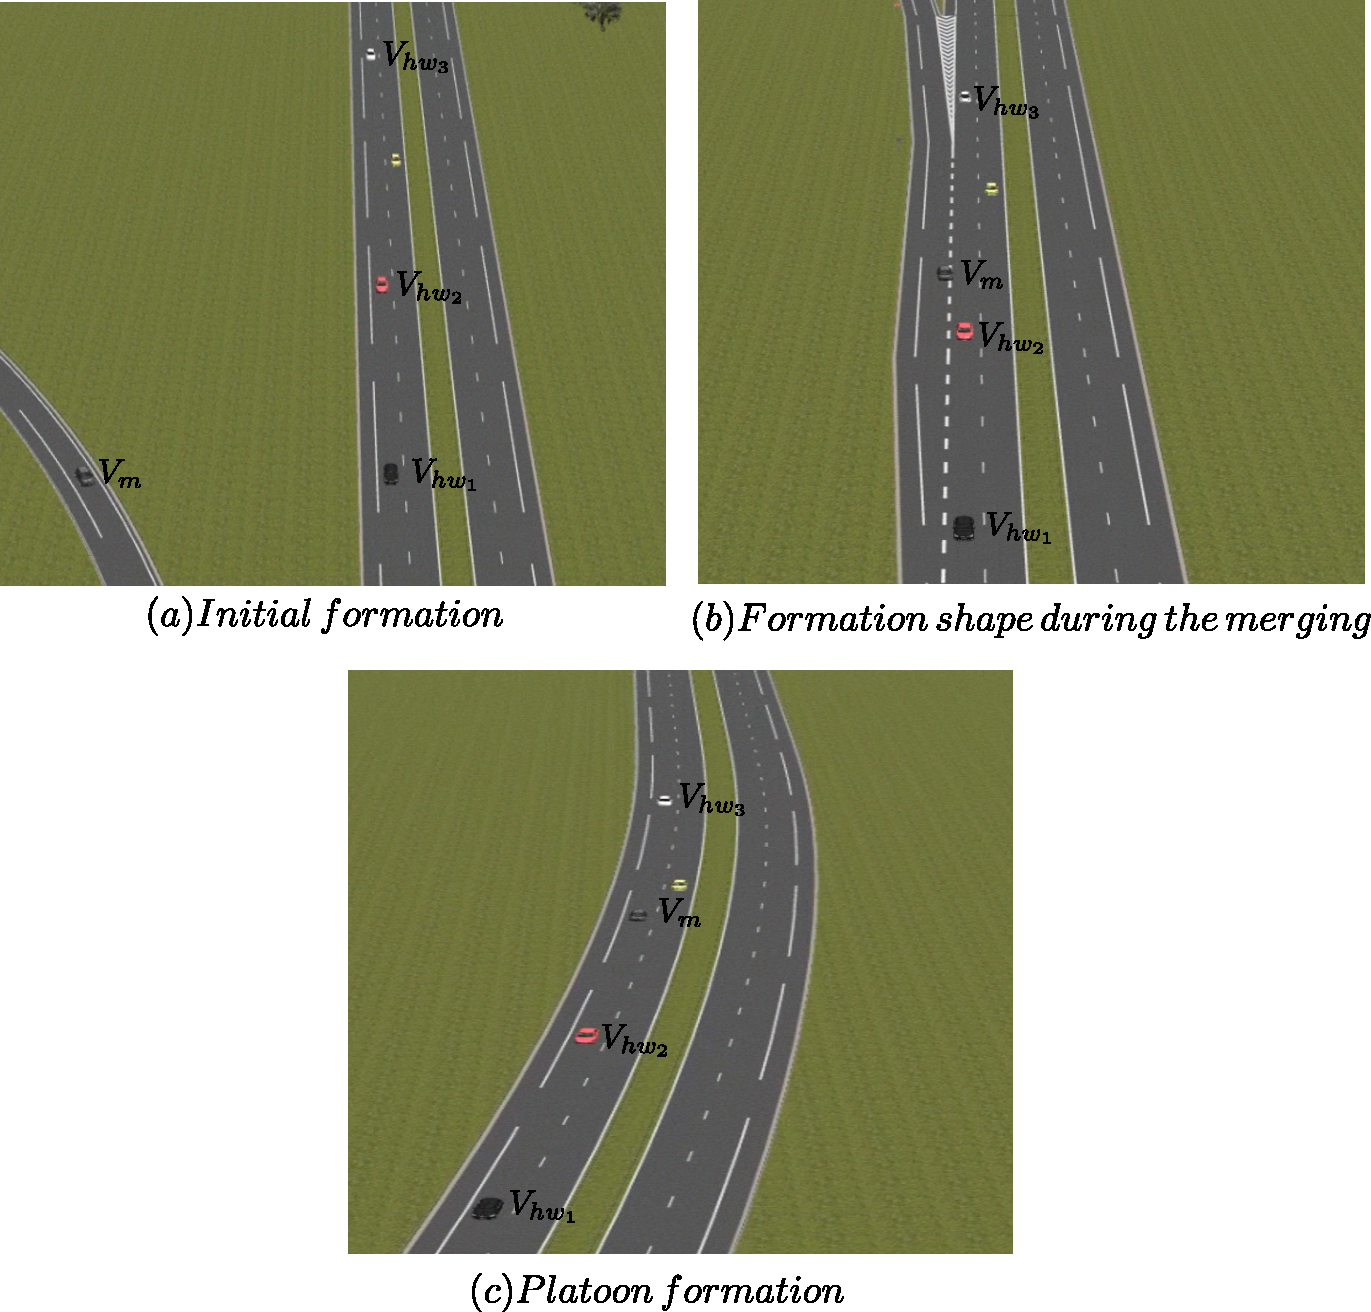
\includegraphics[width=11cm,height=18cm,keepaspectratio]{chapters/Chapitre_5/Figures/FRA-OCS/Formation_shape.pdf}
       % \vspace{-2.3mm}
        \caption{Snapshots of the evolution of the formation shape during the on-ramp merging scenario obtained with the help of SCANeR studio (\textcolor{blue}{Simulation video: https://youtu.be/3gDSq5L3m-c})}
        \label{fig:FRA-OCS:formation_shape}
       % \vspace{-5mm}
        \end{figure}






The initial position of the merging vehicle is configured to trigger the safety of the formation. The FRA-OCS is expected to merge $V_{m}$ between $V_{hw_2}$ and $V_{hw_3}$, $V_{hw_1}$ being the reference vehicle $V_R$ (cf. Figure \ref{fig:FRA-OCS:formation_shape} (b)). The desired formation shape is a platoon formation as in Figure \ref{fig:FRA-OCS:formation_shape} (c).




 

The coordinates of the formation are illustrated in Figure \ref{fig:FRA-OCS:formation_coordinates}. The green and the red shaded zones represent the formation coordinates in Segment $A$ and Segment $B$, respectively. To maintain an appropriate longitudinal separation between the vehicles in the desired formation shape, an inter-vehicle distance corresponding to $\approx 2 [s] \times \mathcal{V} [m/s]$ is employed. Since $V_m$ is placed initially approximately at the same longitudinal position as the reference vehicle $V_R$, its longitudinal coordinate converges from its initial value toward the desired one w.r.t. the Frenet reference frame centered on $V_{hw_1}$ ($V_R$). 


        \begin{figure}[!h]
        \centering 
        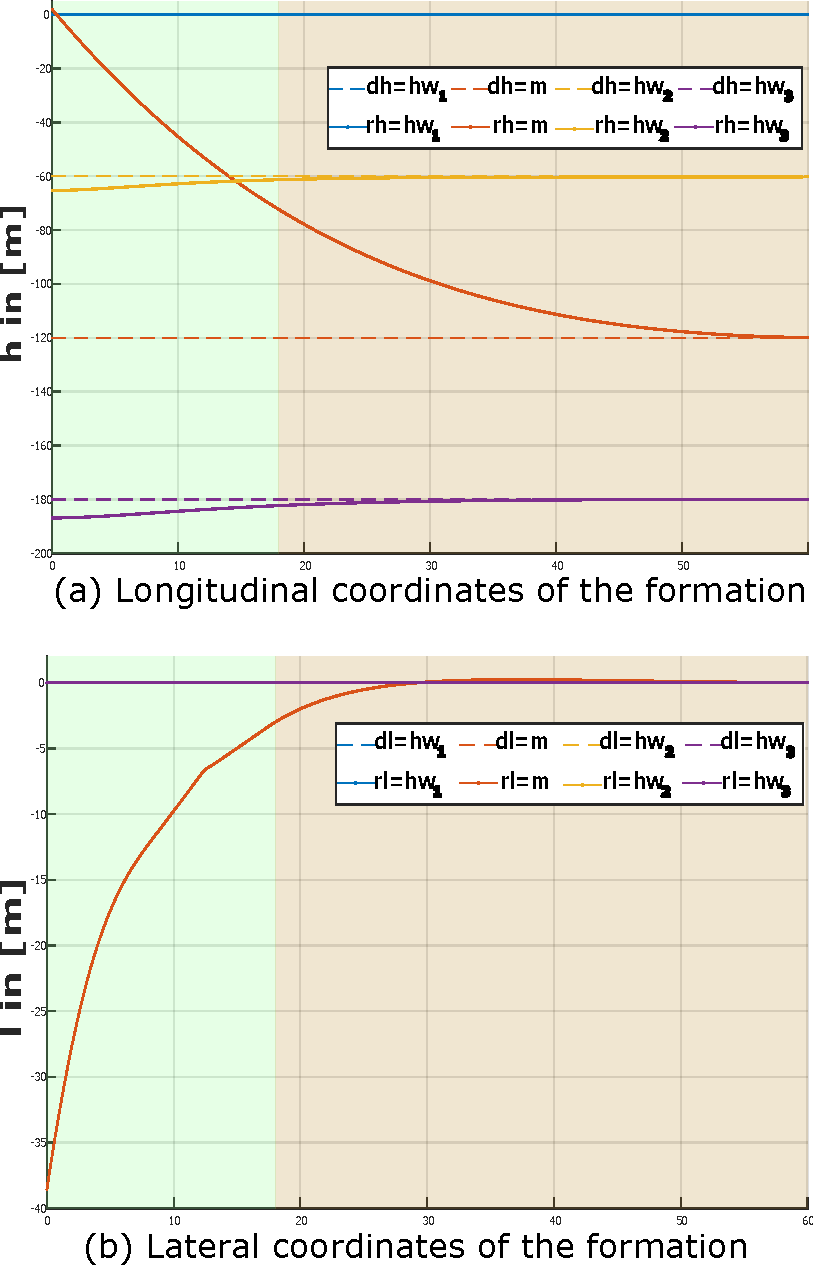
\includegraphics[width=7cm,height=18cm,keepaspectratio]{chapters/Chapitre_5/Figures/FRA-OCS/Coordinates.pdf}
        %\vspace{-2.3mm}
        \caption{The formation's coordinates}
        \label{fig:FRA-OCS:formation_coordinates}
        %\vspace{-5mm}
        \end{figure}



As expected the longitudinal coordinate of the merging vehicle $V_m$ increases toward the desired longitudinal coordinate, such as $V_m$ merges between $V_{hw_2}$ and $V_{hw_3}$. The lateral coordinate of the merging vehicle follows its reference trajectory in Segment $A$, while it is controlled by the inter-target distance matrix in Segment $B$. 


To evaluate the formation's safety during the reconfiguration, the in-between Euclidean distances are depicted in Figure \ref{fig:FRA-OCS:distances}. The minimum Euclidean inter-vehicle distance ${d}_{safe}=\underline{D}_T$ is set to be equal to $10m$. Given the initial placement of $V_m$ w.r.t. $V_{hw_1}$, the Euclidean distance between these two vehicles is below the safety distance before the entry in Segment B, but since they are in two different lanes no collision is occurred. The Euclidean in-between distance increases during the merging while the collision is being solved by the reconfiguration matrix. The rest of the in-between distance plots are all above the safety distance, thus the merging scenario is considered to be safe. 



        \begin{figure}[!h]
        \centering 
        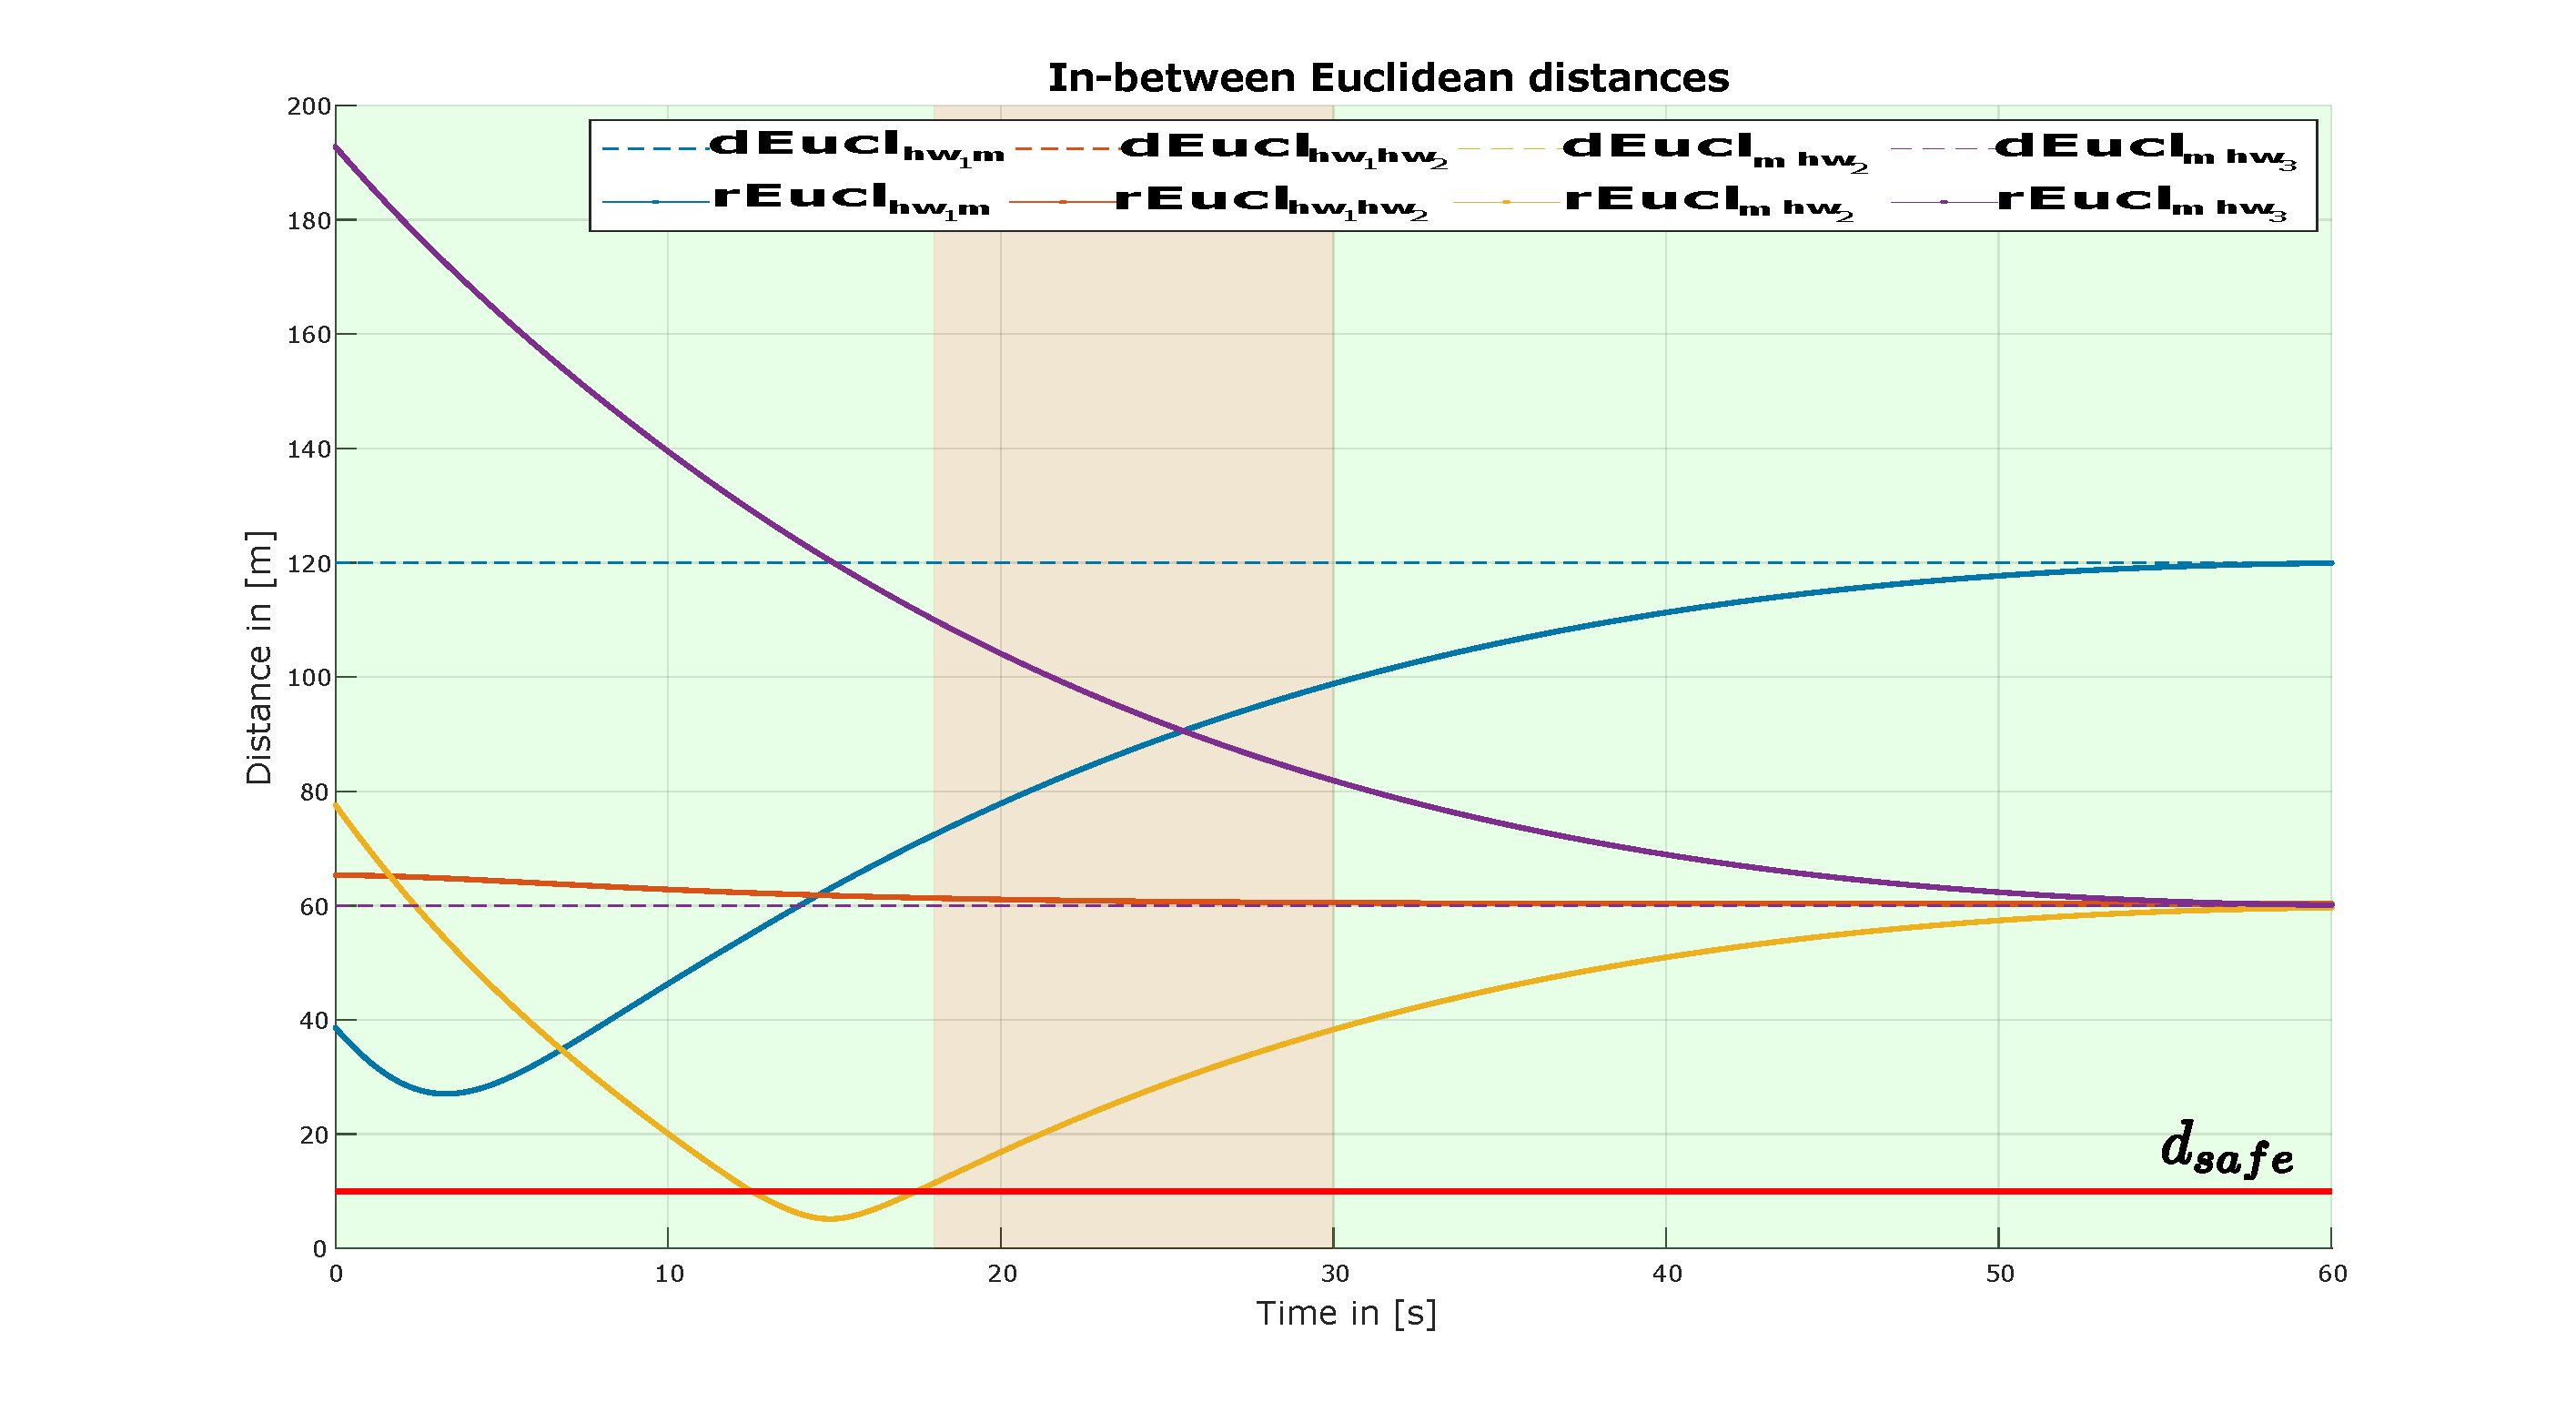
\includegraphics[width=11.5cm,height=18cm,keepaspectratio]{chapters/Chapitre_5/Figures/FRA-OCS/distances.pdf}
        %\vspace{-2.3mm}
        \caption{The Euclidean in-between distances}
        \label{fig:FRA-OCS:distances}
        %\vspace{-5mm}
        \end{figure}

The dynamics of the vehicles during the merging are studied through the velocity profile in Figure \ref{fig:FRA-OCS:velocity}. The initial velocity of the merging vehicle is set to be equal to $60 [km/h]$, smaller than the initial velocity of the highway vehicles (set to be equal to $80 [km/h]$). Both of the velocities of $V_{hw_2}$ and $V_{hw_3}$ increase to reduce the gap w.r.t. the reference vehicle, to decrease afterwards in order to navigate at the same velocity as the reference velocity in order to respect the equal-distance policy part of the platoon requirement.  
        \begin{figure}[!h]
        \centering 
        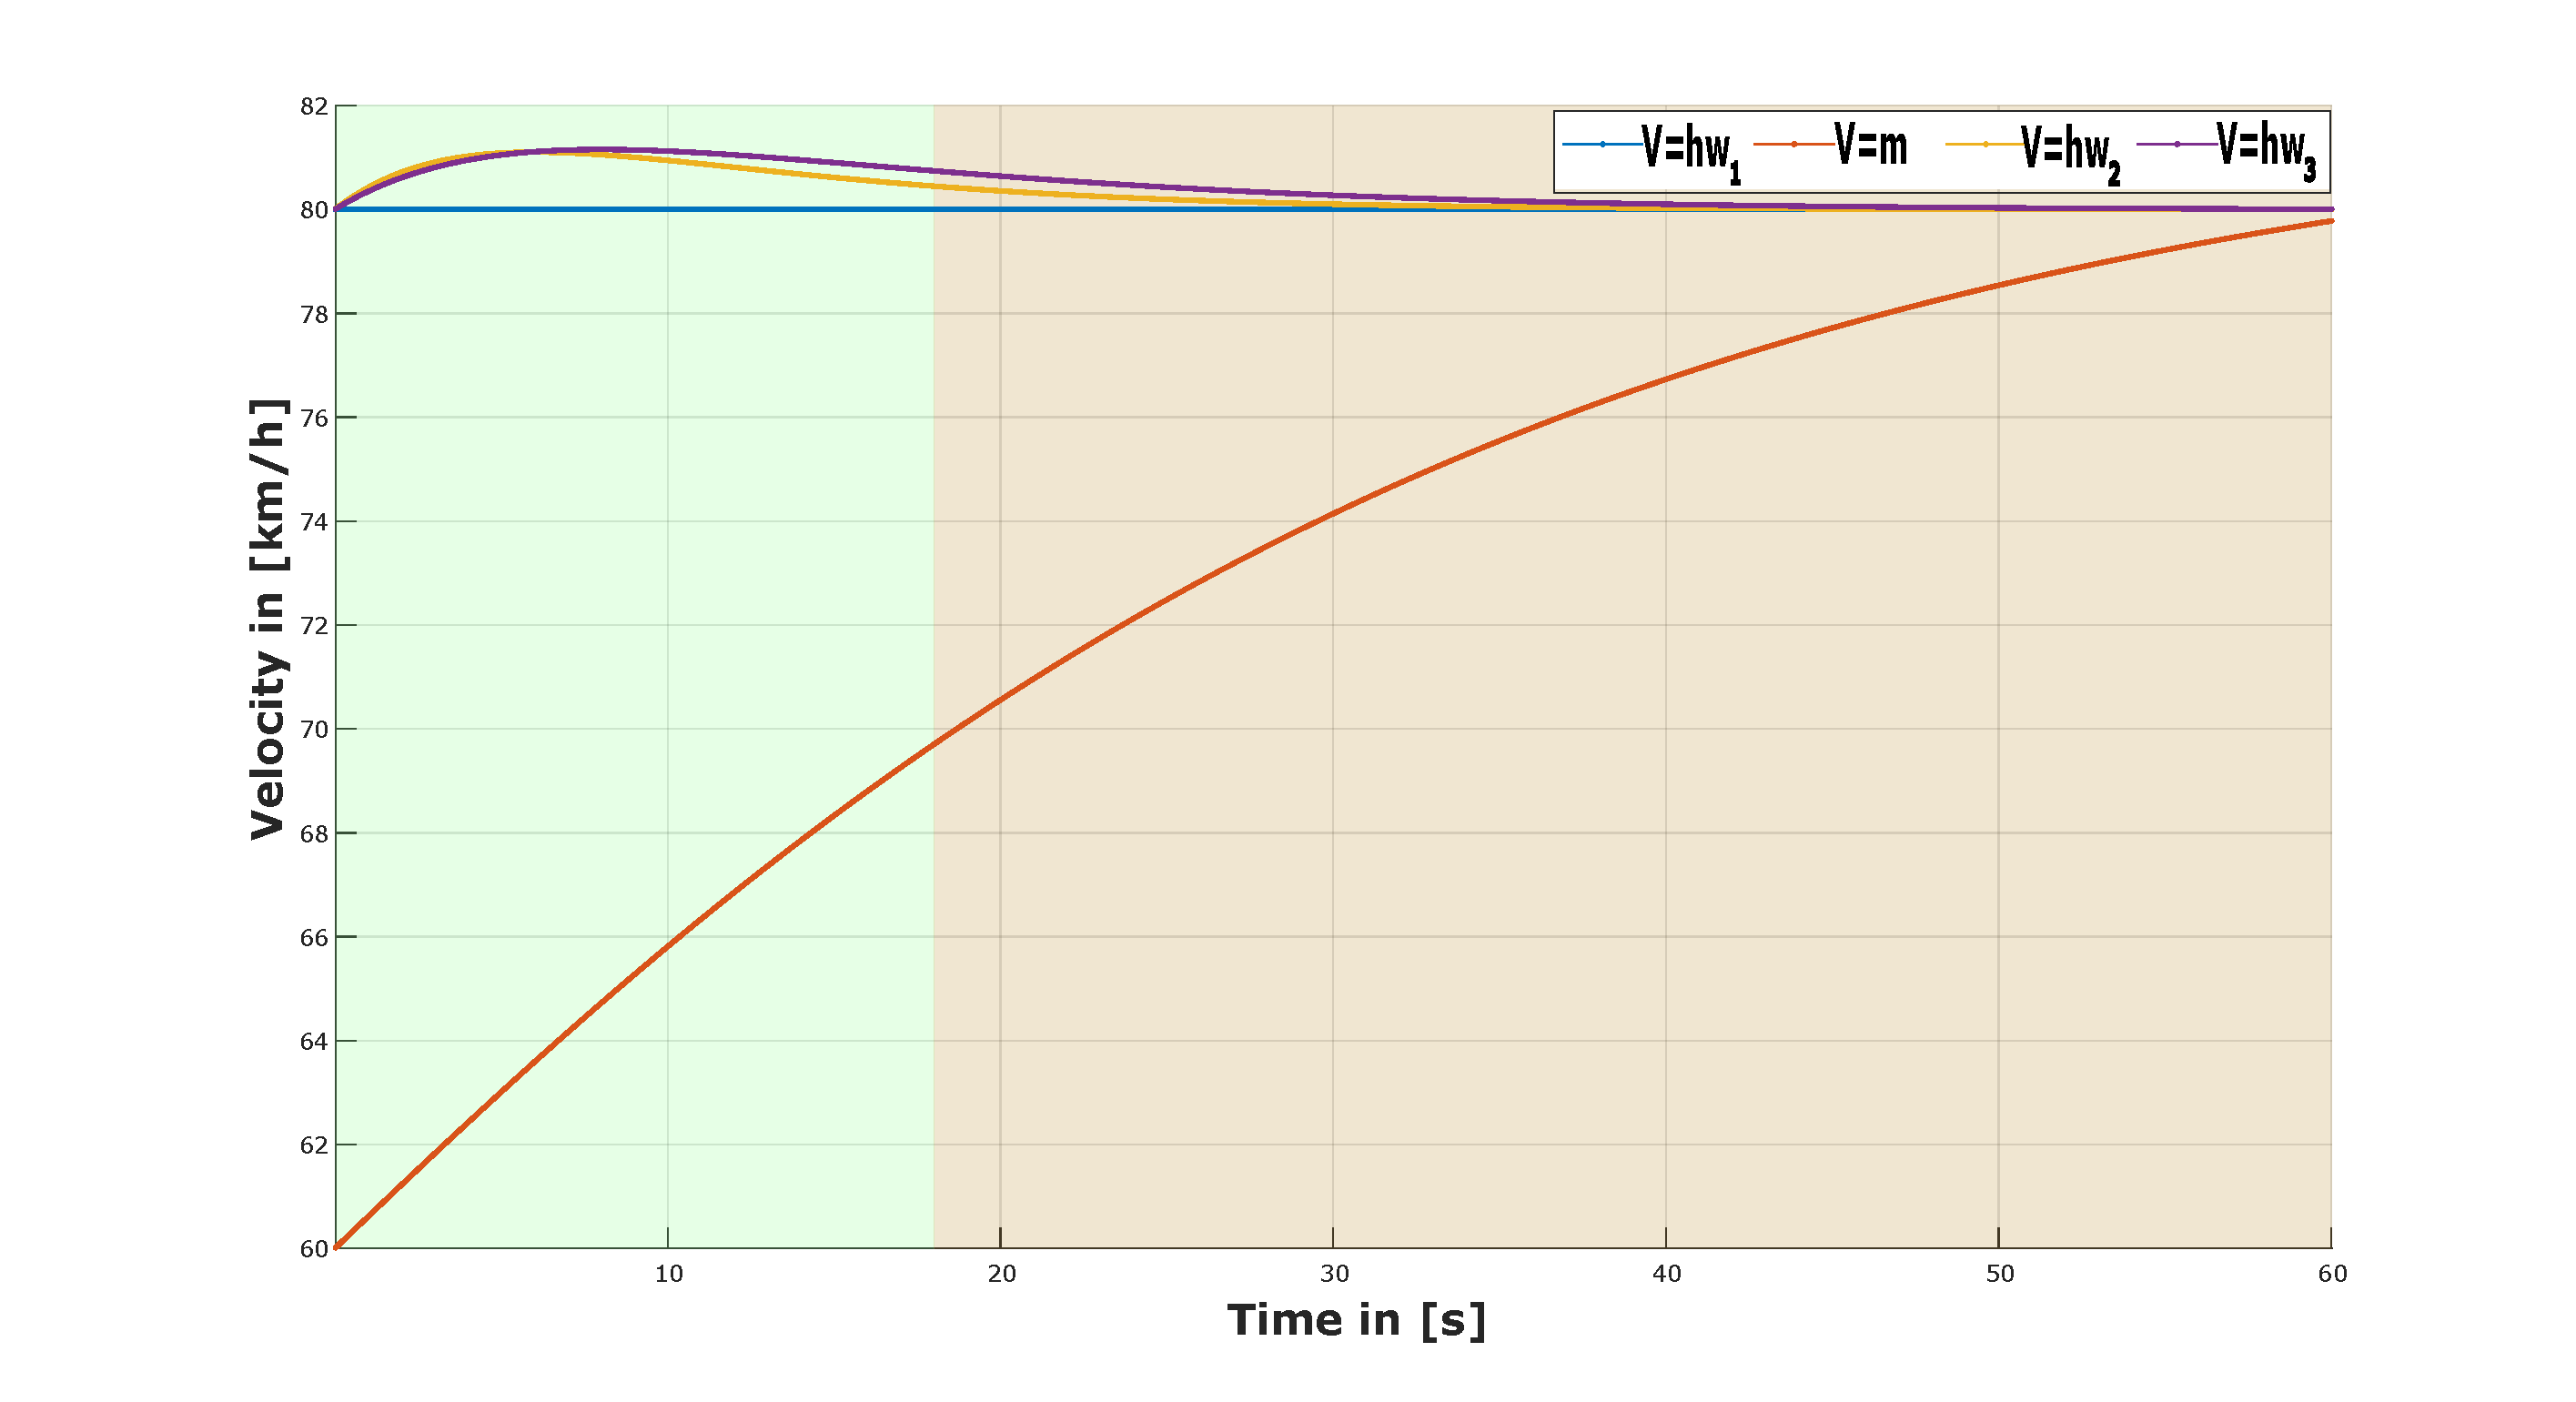
\includegraphics[width=11.5cm,height=18cm,keepaspectratio]{chapters/Chapitre_5/Figures/FRA-OCS/velocity.pdf}
        %\vspace{-2.3mm}
        \caption{The vehicles' velocity profiles}
        \label{fig:FRA-OCS:velocity}
        %\vspace{-5mm}
        \end{figure}

\newpage
\subsection{Conclusion of the FRA-OCS algorithm}\label{sec:Conclusion_FRA-OCS}

Through this section, it was proposed to overcome both of the CORM's and the E-CORM's frameworks limitations. This by introducing the Formation Reconfiguration Approach based on Online Control Strategy (FRA-OCS). 

The proposed FRA-OCS takes advantages from both of the constrained inter-distance matrix and the road segmentation strategy to perform an online formation reconfiguration. In fact, the non-linear optimization algorithm used to compute the reconfiguration matrix during the formation's merging is replaced with an online strategy. A system of equations based on the formalization of the merging scenario, the initial and the final conditions of the vehicles part of the formation was proposed. The latter is solved using a numerical solver to obtain the needed dynamics for each vehicle part of the formation to perform the merging. 

The evaluation of the FRA-OCS algorithm for dynamic formation reconfiguration was carried out in a simulation environment. It showcased the algorithm's ability to adhere to safety criterion and its enhanced flexibility. 










\section{Chapter conclusion} \label{sec:Chapter_Conclusion}

This chapter has extensively examined cooperative formation reconfiguration, presenting and evaluating three distinct frameworks: the Constrained Optimal Reconfiguration Matrix (CORM), the Extended Constrained Optimal Reconfiguration Matrix (E-CORM), and the Formation Reconfiguration Approach based on Online Control Strategy (FRA-OCS).

The CORM framework employs two-step process, utilizing an optimization algorithm to account for environment constraints and a projection approach for safe and feasible merging. While simulation evaluations demonstrated its success in challenging scenarios, it was acknowledged that the CORM has limitations, such as assuming identical dynamics for longitudinal and lateral reconfiguration, impacting its flexibility. 

Introducing the E-CORM aimed to address the CORM's lack of flexibility. The extended inter-target distance matrix and road segmentation strategy enhanced motion flexibility, allowing vehicles to precisely follow their global reference path. Evaluation in a simulation environment showcased the algorithm's enhanced flexibility, but reliance on a non-linear optimization algorithm remained a limitation. 

In response to the limitations of the CORM and the E-CORM, the FRA-OCS was proposed. This approach combines the constrained inter-target distance matrix and road segmentation strategy for online formation reconfiguration. By replacing the non-linear algorithm with an online strategy based on numerically solving of a system of equations, the FRA-OCS demonstrated success in dynamic formation reconfiguration in simulation environments. 


While each framework exhibits strengths, it is essential to recognize their specific limitations. CORM faced challenges with different dynamics in longitudinal and lateral reconfiguration, while both of the CORM and the E-CORM relied on a time-consuming optimization algorithm. Additionally, the FRA-OCS is the formation reconfiguration that met the C-MCA objectives. 

The formation reconfiguration mechanism part of the planning level translates the passing sequence provided by the decision-making level to perform the merging. The following chapter delves in the multi-behavior decision-making strategy used by the decision-making level part of the C-MCA to provide this passing sequence. 